% Pokud existuje soubor config, použiji konfiguraci z něj
\IfFileExists{./config.tex}{% Odkomentováním se povolí zvýrazňování vybraných skladeb
% \def\zvyraznitPovoleno{}

% Odkomentováním se zapne číslování stránek
\def\cislovaniStranekPovoleno{}

% Odkomentováním se vypnutí černá barva pro odkazy (vhodné k tisku)
% \def\cerneOdkazyPovoleno{}

% Odkomentováním se vypnutí černá barva pro veškerý text (vhodné k tisku na černobílé tiskárně). Již není nutné definovat \cernobilyObsahPovoleno
% \def\cernobilyTextPovoleno{}
}
{
%%%%%%%%%%%%%%%%%%%%%%%%%%%%%%%%%%%%%%%%%%%%%%%%%%%%%%%%%%%%%%%%%%%%%%%%%
%%%%%%%%%%%%%%%%%%%%%%%%%%%%%% KONFIGURACE %%%%%%%%%%%%%%%%%%%%%%%%%%%%%%
%%%%%%%%%%%%%%%%%%%%%%%%%%%%%%%%%%%%%%%%%%%%%%%%%%%%%%%%%%%%%%%%%%%%%%%%%
% Odkomentováním se povolí zvýrazňování vybraných skladeb
\def\zvyraznitPovoleno{}

% Odkomentováním se zapne číslování stránek
% \def\cislovaniStranekPovoleno{}

% Odkomentováním se vypnutí černá barva pro odkazy (vhodné k tisku)
\def\cerneOdkazyPovoleno{}

% Odkomentováním se vypnutí černá barva pro veškerý text (vhodné k tisku na černobílé tiskárně). Již není nutné definovat \cernobilyObsahPovoleno
% \def\cernobilyTextPovoleno{}

%%%%%%%%%%%%%%%%%%%%%%%%%%%%%%%%% KONEC %%%%%%%%%%%%%%%%%%%%%%%%%%%%%%%%%
}

% Pokud je nastaven černobílý tisk, zapnu černé odkazy
\ifx\cernobilyTextPovoleno\undefined
\else
	\def\cerneOdkazyPovoleno{}
\fi


\documentclass[a5paper, 10pt, onecolumn]{article}
\usepackage[T1]{fontenc}
% Instal arev package in MikTeX:
% initexmf -u
% initexmf --mkmaps
\usepackage{arev} % \fontencoding{T1}\fontfamily{fav}
\usepackage{aurical} % \Fontskrivan
\usepackage[czech]{babel}
\usepackage{lmodern}
% A5 = 148 x 210
\usepackage[text={132mm, 180mm},left=8mm,top=1cm]{geometry}
\usepackage{graphicx}
\usepackage[dvipsnames]{xcolor}
\usepackage{anyfontsize}
\usepackage{qrcode}
\usepackage[pdftex, hidelinks]{hyperref}
\usepackage{hmaty}
% Skryji tečky v obsahu, pokud je vypnuto čříslování stránek
\ifx\cislovaniStranekPovoleno\undefined
	\usepackage[titles]{tocloft}
	\renewcommand{\cftdot}{}
\fi

% Povolim barevné odkazy pouze pokud je to požadováno
\ifx\cerneOdkazyPovoleno\undefined
	\hypersetup{
	    colorlinks = true
	}
\fi


\begin{document}

% Akordy se tisknou nad textem a neovlivnuji ho;
% Hodnota druheho parametru ovlivnuje zpusob tisku:
%   n - normalni - Akord se tiskne nad textem a neovlivnuje ho
%   s - siroky -
%

\newlength{\sirkaak}
\newcommand{\akord}[1]{\raisebox{\baselineskip}[25pt]{\bf #1}%
                       \settowidth{\sirkaak}{\bf #1}\hspace{-\sirkaak}}

\newcommand{\akordhmat}[1]{\raisebox{-0.2\baselineskip}{\bf #1}}

\newcommand{\sirokyakord}[3]{\raisebox{\baselineskip}{\bf #1~}\settowidth{\sirkaak}{\bf #1~}\hspace{-\sirkaak}%
                             \makebox[\sirkaak][s]{#2 #3 }}


\newcommand{\akordMi}{mi}
\newcommand{\akordCtyri}{$^4$}
\newcommand{\akordSedm}{$^7$}
\newcommand{\akordSest}{$^6$}
\newcommand{\akordMiSest}{mi$^6$}
\newcommand{\akordMiSedm}{mi$^7$}
\newcommand{\akordIs}{$^\#$}
\newcommand{\akordIsSest}{$^\#$$^6$}
\newcommand{\akordIsSedm}{$^\#$$^7$}
\newcommand{\akordIsMi}{$^\#$mi}
\newcommand{\akordIsMiSedm}{$^\#$$^7$mi}
\newcommand{\akordEs}{$^b$}
\newcommand{\akordEsSedm}{$^b$$^7$}
\newcommand{\akordEsMi}{$^b$mi}
\newcommand{\akordEsMiSedm}{$^b$$^7$mi}
\newcommand{\akordMajSedm}{maj$^7$}
\newcommand{\akordDim}{dim}
\newcommand{\akordIsDim}{$^\#$dim}
\newcommand{\akordSusDva}{sus$^2$}
\newcommand{\akordIsSusDva}{$^\#$sus$^2$}
\newcommand{\akordSusCtyri}{sus$^4$}
\newcommand{\akordAddDva}{add$^2$}
\newcommand{\akordAddCtyri}{add$^4$}
\newcommand{\akordAddDevet}{add$^9$}
\newcommand{\akordAddCtyriAddDva}{add$^4$/add$^2$}


%%%%%%%%%%%%%%%%%%%%%%%%%%%%%%%%%%%%%%%%%%%%%%%%%%%%%%%%%%%%%%%%%%%%%
%%%%%%%%%%%%%%%%%%%%%%            C            %%%%%%%%%%%%%%%%%%%%%%
%%%%%%%%%%%%%%%%%%%%%%%%%%%%%%%%%%%%%%%%%%%%%%%%%%%%%%%%%%%%%%%%%%%%%

\newcommand{\C}{\akord{C}}
\newcommand{\Cmi}{\akord{C\akordMi}}
\newcommand{\CSedm}{\akord{C\akordSedm}}
\newcommand{\CSest}{\akord{C\akordSest}}
\newcommand{\CmiSedm}{\akord{C\akordMiSedm}}
\newcommand{\Cis}{\akord{C\akordIs}}
\newcommand{\CisSedm}{\akord{C\akordIsSedm}}
\newcommand{\CisMi}{\akord{C\akordIsMi}}
\newcommand{\CisMiSedm}{\akord{C\akordIsMiSedm}}
\newcommand{\Ces}{\akord{C\akordEs}}
\newcommand{\CesSedm}{\akord{C\akordEsSedm}}
\newcommand{\CesMi}{\akord{C\akordEsMi}}
\newcommand{\CesMiSedm}{\akord{C\akordEsMiSedm}}
\newcommand{\CmajSedm}{\akord{C\akordMajSedm}}
\newcommand{\Cdim}{\akord{C\akordDim}}
\newcommand{\CisDim}{\akord{C\akordIsDim}}
\newcommand{\CsusDva}{\akord{C\akordSusDva}}
\newcommand{\CsusCtyri}{\akord{C\akordSusCtyri}}
\newcommand{\CisSusDva}{\akord{C\akordIsSusDva}}

\newcommand{\CSiroky}{\sirokyakord{C}{}{}}
\newcommand{\CmiSiroky}{\sirokyakord{C\akordMi}{}{}}
\newcommand{\CSedmSiroky}{\sirokyakord{C\akordSedm}{}{}}
\newcommand{\CSestSiroky}{\sirokyakord{C\akordSest}{}{}}
\newcommand{\CmiSedmSiroky}{\sirokyakord{C\akordMiSedm}{}{}}
\newcommand{\CisSiroky}{\sirokyakord{C\akordIs}{}{}}
\newcommand{\CisSedmSiroky}{\sirokyakord{C\akordIsSedm}{}{}}
\newcommand{\CisMiSiroky}{\sirokyakord{C\akordIsMi}{}{}}
\newcommand{\CisMiSedmSiroky}{\sirokyakord{C\akordIsMiSedm}{}{}}
\newcommand{\CesSiroky}{\sirokyakord{}{}{C\akordEs}}
\newcommand{\CesSedmSiroky}{\sirokyakord{C\akordEsSedm}{}{}}
\newcommand{\CesMiSedmSiroky}{\sirokyakord{C\akordEsMiSedm}{}{}}
\newcommand{\CmajSedmSiroky}{\sirokyakord{C\akordMajSedm}{}{}}
\newcommand{\CdimSiroky}{\sirokyakord{}{}{C\akordDim}}
\newcommand{\CisDimSiroky}{\sirokyakord{}{}{C\akordIsDim}}
\newcommand{\CsusDvaSiroky}{\sirokyakord{C\akordSusDva}{}{}}
\newcommand{\CsusCtyriSiroky}{\sirokyakord{C\akordSusCtyri}{}{}}
\newcommand{\CisSusDvaSiroky}{\sirokyakord{C\akordIsSusDva}{}{}}



%%%%%%%%%%%%%%%%%%%%%%%%%%%%%%%%%%%%%%%%%%%%%%%%%%%%%%%%%%%%%%%%%%%%%
%%%%%%%%%%%%%%%%%%%%%%            D            %%%%%%%%%%%%%%%%%%%%%%
%%%%%%%%%%%%%%%%%%%%%%%%%%%%%%%%%%%%%%%%%%%%%%%%%%%%%%%%%%%%%%%%%%%%%

\newcommand{\D}{\akord{D}}
\newcommand{\Dmi}{\akord{D\akordMi}}
\newcommand{\DSedm}{\akord{D\akordSedm}}
\newcommand{\DSest}{\akord{D\akordSest}}
\newcommand{\DmiSedm}{\akord{D\akordMiSedm}}
\newcommand{\Dis}{\akord{D\akordIs}}
\newcommand{\DisSedm}{\akord{D\akordIsSedm}}
\newcommand{\DisMi}{\akord{D\akordIsMi}}
\newcommand{\DisMiSedm}{\akord{D\akordIsMiSedm}}
\newcommand{\Des}{\akord{D\akordEs}}
\newcommand{\DesSedm}{\akord{D\akordEsSedm}}
\newcommand{\DesMi}{\akord{D\akordEsMi}}
\newcommand{\DesMiSedm}{\akord{D\akordEsMiSedm}}
\newcommand{\DmajSedm}{\akord{D\akordMajSedm}}
\newcommand{\Ddim}{\akord{D\akordDim}}
\newcommand{\DisDim}{\akord{D\akordIsDim}}
\newcommand{\DsusDva}{\akord{D\akordSusDva}}
\newcommand{\DsusCtyri}{\akord{D\akordSusCtyri}}
\newcommand{\DCtyri}{\akord{D\akordCtyri}}


\newcommand{\DSiroky}{\sirokyakord{D}{}{}}
\newcommand{\DmiSiroky}{\sirokyakord{D\akordMi}{}{}}
\newcommand{\DSedmSiroky}{\sirokyakord{D\akordSedm}{}{}}
\newcommand{\DSestSiroky}{\sirokyakord{D\akordSest}{}{}}
\newcommand{\DmiSedmSiroky}{\sirokyakord{D\akordMiSedm}{}{}}
\newcommand{\DisSiroky}{\sirokyakord{D\akordIs}{}{}}
\newcommand{\DisSedmSiroky}{\sirokyakord{D\akordIsSedm}{}{}}
\newcommand{\DisMiSiroky}{\sirokyakord{D\akordIsMi}{}{}}
\newcommand{\DisMiSedmSiroky}{\sirokyakord{D\akordIsMiSedm}{}{}}
\newcommand{\DesSiroky}{\sirokyakord{}{}{D\akordEs}}
\newcommand{\DesSedmSiroky}{\sirokyakord{D\akordEsSedm}{}{}}
\newcommand{\DesMiSedmSiroky}{\sirokyakord{D\akordEsMiSedm}{}{}}
\newcommand{\DmajSedmSiroky}{\sirokyakord{D\akordMajSedm}{}{}}
\newcommand{\DdimSiroky}{\sirokyakord{}{}{D\akordDim}}
\newcommand{\DisDimSiroky}{\sirokyakord{}{}{D\akordIsDim}}
\newcommand{\DsusDvaSiroky}{\sirokyakord{D\akordSusDva}{}{}}
\newcommand{\DsusCtyriSiroky}{\sirokyakord{D\akordSusCtyri}{}{}}
\newcommand{\DCtyriSiroky}{\sirokyakord{D\akordCtyri}{}{}}



%%%%%%%%%%%%%%%%%%%%%%%%%%%%%%%%%%%%%%%%%%%%%%%%%%%%%%%%%%%%%%%%%%%%%
%%%%%%%%%%%%%%%%%%%%%%            E            %%%%%%%%%%%%%%%%%%%%%%
%%%%%%%%%%%%%%%%%%%%%%%%%%%%%%%%%%%%%%%%%%%%%%%%%%%%%%%%%%%%%%%%%%%%%

\newcommand{\E}{\akord{E}}
\newcommand{\Emi}{\akord{E\akordMi}}
\newcommand{\ESedm}{\akord{E\akordSedm}}
\newcommand{\ESest}{\akord{E\akordSest}}
\newcommand{\EmiSedm}{\akord{E\akordMiSedm}}
\newcommand{\Eis}{\akord{E\akordIs}}
\newcommand{\EisSedm}{\akord{E\akordIsSedm}}
\newcommand{\EisMi}{\akord{E\akordIsMi}}
\newcommand{\EisMiSedm}{\akord{E\akordIsMiSedm}}
\newcommand{\Ees}{\akord{E\akordEs}}
\newcommand{\EesSedm}{\akord{E\akordEsSedm}}
\newcommand{\EesMi}{\akord{E\akordEsMi}}
\newcommand{\EesMiSedm}{\akord{E\akordEsMiSedm}}
\newcommand{\EmajSedm}{\akord{E\akordMajSedm}}
\newcommand{\Edim}{\akord{E\akordDim}}
\newcommand{\EisDim}{\akord{E\akordIsDim}}
\newcommand{\EsusDva}{\akord{E\akordSusDva}}
\newcommand{\EsusCtyri}{\akord{E\akordSusCtyri}}

\newcommand{\ESiroky}{\sirokyakord{E}{}{}}
\newcommand{\EmiSiroky}{\sirokyakord{E\akordMi}{}{}}
\newcommand{\ESedmSiroky}{\sirokyakord{E\akordSedm}{}{}}
\newcommand{\ESestSiroky}{\sirokyakord{E\akordSest}{}{}}
\newcommand{\EmiSedmSiroky}{\sirokyakord{E\akordMiSedm}{}{}}
\newcommand{\EisSiroky}{\sirokyakord{E\akordIs}{}{}}
\newcommand{\EisSedmSiroky}{\sirokyakord{E\akordIsSedm}{}{}}
\newcommand{\EisMiSiroky}{\sirokyakord{E\akordIsMi}{}{}}
\newcommand{\EisMiSedmSiroky}{\sirokyakord{E\akordIsMiSedm}{}{}}
\newcommand{\EesSiroky}{\sirokyakord{}{}{E\akordEs}}
\newcommand{\EesSedmSiroky}{\sirokyakord{E\akordEsSedm}{}{}}
\newcommand{\EesMiSedmSiroky}{\sirokyakord{E\akordEsMiSedm}{}{}}
\newcommand{\EmajSedmSiroky}{\sirokyakord{E\akordMajSedm}{}{}}
\newcommand{\EdimSiroky}{\sirokyakord{}{}{E\akordDim}}
\newcommand{\EIsimSiroky}{\sirokyakord{}{}{E\akordIsDim}}
\newcommand{\EsusDvaSiroky}{\sirokyakord{E\akordSusDva}{}{}}
\newcommand{\EsusCtyriSiroky}{\sirokyakord{E\akordSusCtyri}{}{}}



%%%%%%%%%%%%%%%%%%%%%%%%%%%%%%%%%%%%%%%%%%%%%%%%%%%%%%%%%%%%%%%%%%%%%
%%%%%%%%%%%%%%%%%%%%%%            F            %%%%%%%%%%%%%%%%%%%%%%
%%%%%%%%%%%%%%%%%%%%%%%%%%%%%%%%%%%%%%%%%%%%%%%%%%%%%%%%%%%%%%%%%%%%%

\newcommand{\F}{\akord{F}}
\newcommand{\Fmi}{\akord{F\akordMi}}
\newcommand{\FSedm}{\akord{F\akordSedm}}
\newcommand{\FSest}{\akord{F\akordSest}}
\newcommand{\FmiSest}{\akord{F\akordMiSest}}
\newcommand{\FmiSedm}{\akord{F\akordMiSedm}}
\newcommand{\Fis}{\akord{F\akordIs}}
\newcommand{\FisSest}{\akord{F\akordIsSest}}
\newcommand{\FisSedm}{\akord{F\akordIsSedm}}
\newcommand{\FisMi}{\akord{F\akordIsMi}}
\newcommand{\FisMiSedm}{\akord{F\akordIsMiSedm}}
\newcommand{\Fes}{\akord{F\akordEs}}
\newcommand{\FesSedm}{\akord{F\akordEsSedm}}
\newcommand{\FesMi}{\akord{F\akordEsMi}}
\newcommand{\FesMiSedm}{\akord{F\akordEsMiSedm}}
\newcommand{\FmajSedm}{\akord{F\akordMajSedm}}
\newcommand{\Fdim}{\akord{F\akordDim}}
\newcommand{\FisDim}{\akord{F\akordIsDim}}
\newcommand{\FsusDva}{\akord{F\akordSusDva}}
\newcommand{\FsusCtyri}{\akord{F\akordSusCtyri}}

\newcommand{\FSiroky}{\sirokyakord{F}{}{}}
\newcommand{\FmiSiroky}{\sirokyakord{F\akordMi}{}{}}
\newcommand{\FSedmSiroky}{\sirokyakord{F\akordSedm}{}{}}
\newcommand{\FSestSiroky}{\sirokyakord{F\akordSest}{}{}}
\newcommand{\FmiSedmSiroky}{\sirokyakord{F\akordMiSedm}{}{}}
\newcommand{\FisSiroky}{\sirokyakord{F\akordIs}{}{}}
\newcommand{\FisSedmSiroky}{\sirokyakord{F\akordIsSedm}{}{}}
\newcommand{\FisMiSiroky}{\sirokyakord{F\akordIsMi}{}{}}
\newcommand{\FisMiSedmSiroky}{\sirokyakord{F\akordIsMiSedm}{}{}}
\newcommand{\FesSiroky}{\sirokyakord{}{}{F\akordEs}}
\newcommand{\FesSedmSiroky}{\sirokyakord{F\akordEsSedm}{}{}}
\newcommand{\FesMiSedmSiroky}{\sirokyakord{F\akordEsMiSedm}{}{}}
\newcommand{\FmajSedmSiroky}{\sirokyakord{F\akordMajSedm}{}{}}
\newcommand{\FdimSiroky}{\sirokyakord{}{}{F\akordDim}}
\newcommand{\FisDimSiroky}{\sirokyakord{}{}{F\akordIsDim}}
\newcommand{\FsusDvaSiroky}{\sirokyakord{F\akordSusDva}{}{}}
\newcommand{\FsusCtyriSiroky}{\sirokyakord{F\akordSusCtyri}{}{}}



%%%%%%%%%%%%%%%%%%%%%%%%%%%%%%%%%%%%%%%%%%%%%%%%%%%%%%%%%%%%%%%%%%%%%
%%%%%%%%%%%%%%%%%%%%%%            G            %%%%%%%%%%%%%%%%%%%%%%
%%%%%%%%%%%%%%%%%%%%%%%%%%%%%%%%%%%%%%%%%%%%%%%%%%%%%%%%%%%%%%%%%%%%%

\newcommand{\G}{\akord{G}}
\newcommand{\Gmi}{\akord{G\akordMi}}
\newcommand{\GSedm}{\akord{G\akordSedm}}
\newcommand{\GSest}{\akord{G\akordSest}}
\newcommand{\GmiSedm}{\akord{G\akordMiSedm}}
\newcommand{\Gis}{\akord{G\akordIs}}
\newcommand{\GisSedm}{\akord{G\akordIsSedm}}
\newcommand{\GisMi}{\akord{G\akordIsMi}}
\newcommand{\GisMiSedm}{\akord{G\akordIsMiSedm}}
\newcommand{\Ges}{\akord{G\akordEs}}
\newcommand{\GesSedm}{\akord{G\akordEsSedm}}
\newcommand{\GesMi}{\akord{G\akordEsMi}}
\newcommand{\GesMiSedm}{\akord{G\akordEsMiSedm}}
\newcommand{\GmajSedm}{\akord{G\akordMajSedm}}
\newcommand{\Gdim}{\akord{G\akordDim}}
\newcommand{\GisDim}{\akord{G\akordIsDim}}
\newcommand{\GsusDva}{\akord{G\akordSusDva}}
\newcommand{\GsusCtyri}{\akord{G\akordSusCtyri}}

\newcommand{\GSiroky}{\sirokyakord{G}{}{}}
\newcommand{\GmiSiroky}{\sirokyakord{G\akordMi}{}{}}
\newcommand{\GSedmSiroky}{\sirokyakord{G\akordSedm}{}{}}
\newcommand{\GSestSiroky}{\sirokyakord{G\akordSest}{}{}}
\newcommand{\GmiSedmSiroky}{\sirokyakord{G\akordMiSedm}{}{}}
\newcommand{\GisSiroky}{\sirokyakord{G\akordIs}{}{}}
\newcommand{\GisSedmSiroky}{\sirokyakord{G\akordIsSedm}{}{}}
\newcommand{\GisMiSiroky}{\sirokyakord{G\akordIsMi}{}{}}
\newcommand{\GisMiSedmSiroky}{\sirokyakord{G\akordIsMiSedm}{}{}}
\newcommand{\GesSiroky}{\sirokyakord{}{}{G\akordEs}}
\newcommand{\GesSedmSiroky}{\sirokyakord{G\akordEsSedm}{}{}}
\newcommand{\GesMiSedmSiroky}{\sirokyakord{G\akordEsMiSedm}{}{}}
\newcommand{\GmajSedmSiroky}{\sirokyakord{G\akordMajSedm}{}{}}
\newcommand{\GdimSiroky}{\sirokyakord{}{}{G\akordDim}}
\newcommand{\GisDimSiroky}{\sirokyakord{}{}{G\akordIsDim}}
\newcommand{\GsusDvaSiroky}{\sirokyakord{G\akordSusDva}{}{}}
\newcommand{\GsusCtyriSiroky}{\sirokyakord{G\akordSusCtyri}{}{}}



%%%%%%%%%%%%%%%%%%%%%%%%%%%%%%%%%%%%%%%%%%%%%%%%%%%%%%%%%%%%%%%%%%%%%
%%%%%%%%%%%%%%%%%%%%%%            A            %%%%%%%%%%%%%%%%%%%%%%
%%%%%%%%%%%%%%%%%%%%%%%%%%%%%%%%%%%%%%%%%%%%%%%%%%%%%%%%%%%%%%%%%%%%%

\newcommand{\A}{\akord{A}}
\newcommand{\Ami}{\akord{A\akordMi}}
\newcommand{\ASedm}{\akord{A\akordSedm}}
\newcommand{\ASest}{\akord{A\akordSest}}
\newcommand{\AmiSedm}{\akord{A\akordMiSedm}}
\newcommand{\B}{\akord{B}}
\newcommand{\BSedm}{\akord{B\akordSedm}}
\newcommand{\BMi}{\akord{B\akordMi}}
\newcommand{\BMiSedm}{\akord{B\akordMiSedm}}
\newcommand{\Aes}{\akord{A\akordEs}}
\newcommand{\AesSedm}{\akord{A\akordEsSedm}}
\newcommand{\AesMi}{\akord{A\akordEsMi}}
\newcommand{\AesMiSedm}{\akord{A\akordEsMiSedm}}
\newcommand{\AmajSedm}{\akord{A\akordMajSedm}}
\newcommand{\Adim}{\akord{A\akordDim}}
\newcommand{\BDim}{\akord{B\akordDim}}
\newcommand{\AsusDva}{\akord{A\akordSusDva}}
\newcommand{\AsusCtyri}{\akord{A\akordSusCtyri}}
\newcommand{\BsusDva}{\akord{B\akordSusDva}}

\newcommand{\ASiroky}{\sirokyakord{A}{}{}}
\newcommand{\AmiSiroky}{\sirokyakord{A\akordMi}{}{}}
\newcommand{\ASedmSiroky}{\sirokyakord{A\akordSedm}{}{}}
\newcommand{\ASestSiroky}{\sirokyakord{A\akordSest}{}{}}
\newcommand{\AmiSestSiroky}{\sirokyakord{A\akordSest}{}{}}
\newcommand{\AmiSedmSiroky}{\sirokyakord{A\akordMiSedm}{}{}}
\newcommand{\BSiroky}{\sirokyakord{B}{}{}}
\newcommand{\BSedmSiroky}{\sirokyakord{B\akordSedm}{}{}}
\newcommand{\BMiSiroky}{\sirokyakord{B\akordMi}{}{}}
\newcommand{\BMiSedmSiroky}{\sirokyakord{B\akordMiSedm}{}{}}
\newcommand{\AesSiroky}{\sirokyakord{}{}{A\akordEs}}
\newcommand{\AesSedmSiroky}{\sirokyakord{A\akordEsSedm}{}{}}
\newcommand{\AesMiSedmSiroky}{\sirokyakord{A\akordEsMiSedm}{}{}}
\newcommand{\AmajSedmSiroky}{\sirokyakord{A\akordMajSedm}{}{}}
\newcommand{\AdimSiroky}{\sirokyakord{A\akordDim}{}{}}
\newcommand{\BDimSiroky}{\sirokyakord{B\akordDim}{}{}}
\newcommand{\AsusDvaSiroky}{\sirokyakord{A\akordSusDva}{}{}}
\newcommand{\AsusCtyriSiroky}{\sirokyakord{A\akordSusCtyri}{}{}}



%%%%%%%%%%%%%%%%%%%%%%%%%%%%%%%%%%%%%%%%%%%%%%%%%%%%%%%%%%%%%%%%%%%%%
%%%%%%%%%%%%%%%%%%%%%%            H            %%%%%%%%%%%%%%%%%%%%%%
%%%%%%%%%%%%%%%%%%%%%%%%%%%%%%%%%%%%%%%%%%%%%%%%%%%%%%%%%%%%%%%%%%%%%

\newcommand{\Ha}{\akord{H}}
\newcommand{\Hmi}{\akord{H\akordMi}}
\newcommand{\HSedm}{\akord{H\akordSedm}}
\newcommand{\HSest}{\akord{H\akordSest}}
\newcommand{\HmiSedm}{\akord{H\akordMiSedm}}
\newcommand{\His}{\akord{H\akordIs}}
\newcommand{\HisSedm}{\akord{H\akordIsSedm}}
\newcommand{\HisMi}{\akord{H\akordIsMi}}
\newcommand{\HisMiSedm}{\akord{H\akordIsMiSedm}}
\newcommand{\Hes}{\akord{H\akordEs}}
\newcommand{\HesSedm}{\akord{H\akordEsSedm}}
\newcommand{\HesMi}{\akord{H\akordEsMi}}
\newcommand{\HesMiSedm}{\akord{H\akordEsMiSedm}}
\newcommand{\HmajSedm}{\akord{H\akordMajSedm}}
\newcommand{\Hdim}{\akord{H\akordDim}}
\newcommand{\HisDim}{\akord{H\akordIsDim}}
\newcommand{\HsusDva}{\akord{H\akordSusDva}}
\newcommand{\HsusCtyri}{\akord{H\akordSusCtyri}}

\newcommand{\HaSiroky}{\sirokyakord{H}{}{}}
\newcommand{\HmiSiroky}{\sirokyakord{H\akordMi}{}{}}
\newcommand{\HSedmSiroky}{\sirokyakord{H\akordSedm}{}{}}
\newcommand{\HSestSiroky}{\sirokyakord{H\akordSest}{}{}}
\newcommand{\HmiSedmSiroky}{\sirokyakord{H\akordMiSedm}{}{}}
\newcommand{\HisSiroky}{\sirokyakord{H\akordIs}{}{}}
\newcommand{\HisSedmSiroky}{\sirokyakord{H\akordIsSedm}{}{}}
\newcommand{\HisMiSiroky}{\sirokyakord{H\akordIsMi}{}{}}
\newcommand{\HisMiSedmSiroky}{\sirokyakord{H\akordIsMiSedm}{}{}}
\newcommand{\HesSiroky}{\sirokyakord{}{}{H\akordEs}}
\newcommand{\HesSedmSiroky}{\sirokyakord{H\akordEsSedm}{}{}}
\newcommand{\HesMiSedmSiroky}{\sirokyakord{H\akordEsMiSedm}{}{}}
\newcommand{\HmajSedmSiroky}{\sirokyakord{H\akordMajSedm}{}{}}
\newcommand{\HdimSiroky}{\sirokyakord{}{}{H\akordDim}}
\newcommand{\HisDimSiroky}{\sirokyakord{}{}{H\akordDim}}
\newcommand{\HsusDvaSiroky}{\sirokyakord{H\akordSusDva}{}{}}
\newcommand{\HsusCtyriSiroky}{\sirokyakord{H\akordSusCtyri}{}{}}



%%%%%%%%%%%%%%%%%%%%%%%%%%%%%%%%%%%%%%%%%%%%%%%%%%%%%%%%%%%%%%%%%%%%%
%%%%%%%%%%%%%%%%%%%%%%        Specialni        %%%%%%%%%%%%%%%%%%%%%%
%%%%%%%%%%%%%%%%%%%%%%%%%%%%%%%%%%%%%%%%%%%%%%%%%%%%%%%%%%%%%%%%%%%%%
\newcommand{\X}{\akord{.}}
\newcommand{\XSiroky}{\sirokyakord{.}{}{}}

\newcommand{\I}{\akord{|}}
\newcommand{\IX}{\akord{|.}}
\newcommand{\IA}{\akord{|A}}
\newcommand{\IC}{\akord{|C}}
\newcommand{\IF}{\akord{|F}}
\newcommand{\IE}{\akord{|E}}
\newcommand{\IG}{\akord{|G}}
\newcommand{\ID}{\akord{|D}}
\newcommand{\IAmi}{\akord{|A\akordMi}}
\newcommand{\IEmi}{\akord{|E\akordMi}}
\newcommand{\IDmi}{\akord{|D\akordMi}}
\newcommand{\IASedm}{\akord{|A\akordSedm}}
\newcommand{\IDSedm}{\akord{|D\akordSedm}}
\newcommand{\IAsusCtyri}{\akord{|A\akordSusCtyri}}



\newcommand{\AmiG}{\akord{A\akordMi /G}}
\newcommand{\AmiGSiroky}{\sirokyakord{A\akordMi /G}{}{}}

\newcommand{\CH}{\akord{C/H}}
\newcommand{\CHSiroky}{\sirokyakord{C/H}{}{}}
\newcommand{\CmajSedmG}{\akord{C\akordMajSedm/G}}
\newcommand{\CmajSedmGSiroky}{\sirokyakord{C\akordMajSedm/G}{}{}}

\newcommand{\CaddDevet}{\akord{C\akordAddDevet}}
\newcommand{\ICaddDevet}{\akord{|C\akordAddDevet}}
\newcommand{\CaddDevetSiroky}{\sirokyakord{C\akordAddDevet}{}{}}

\newcommand{\DaddCtyriAddDva}{\akord{D\akordAddCtyri/\akordAddDva}}
\newcommand{\DaddCtyriAddDvaSiroky}{\sirokyakord{D\akordAddCtyri/\akordAddDva}{}{}}




%%%%%%%%%%%%%%%%%%%%%%%%%%%%%%%%%%%%%%%%%%%%%%%%%%%%%%%%%%%%%%%%%%%%%
%%%%%%%%%%%%%%%%%%%%            Hmaty            %%%%%%%%%%%%%%%%%%%%
%%%%%%%%%%%%%%%%%%%%%%%%%%%%%%%%%%%%%%%%%%%%%%%%%%%%%%%%%%%%%%%%%%%%%


\newcommand{\hmatCdim}{\hmat[]{x,x,n,p1,n,p1}{\akordhmat{C\akordDim}}}
\newcommand{\hmatGmi}{\hmat[]{p3,p1,n,n,p3,p3}{\akordhmat{G\akordMi}}}
\newcommand{\hmatCmajSedm}{\hmat[]{p3,p3,p2,n,n,n}{\akordhmat{C\akordMajSedm}}}
\newcommand{\hmatCmajSedmD}{\hmat[]{p3,p3,p2,n,n,n}{\akordhmat{C\akordMajSedm}}}
\newcommand{\hmatAmajSedm}{\hmat[]{n,n,p2,p1,p2,n}{\akordhmat{A\akordMajSedm}}}
\newcommand{\hmatFmajSedm}{\hmat[]{n,n,p3,p2,p1,n}{\akordhmat{F\akordMajSedm}}}
\newcommand{\hmatFdim}{\hmat[]{x,x,n,p1,n,p1}{\akordhmat{F\akordDim}}}
\newcommand{\hmatAmiG}{\hmat[]{p3,n,p2,p2,p1,n}{\akordhmat{A\akordMi /G}}}
\newcommand{\hmatDisDim}{\hmat[]{x,x,p3,p4,p3,p4}{\akordhmat{D\akordIsDim}}}
\newcommand{\hmatCH}{\hmat[]{n,p2,p2,n,p1,n}{\akordhmat{C/H}}}
\newcommand{\hmatDsusDva}{\hmat[]{x,x,n,p2,p3,n}{\akordhmat{D\akordSusDva}}}
\newcommand{\hmatHsusDva}{\hmat[b1]{n,n,p3,p3,n,n}{\akordhmat{H\akordSusDva}}}
\newcommand{\hmatFsest}{\hmat[]{n,n,p3,p2,p3,p1}{\akordhmat{F\akordSest}}}
\newcommand{\hmatAsusDva}{\hmat[]{x,x,p2,p2,n,n}{\akordhmat{A\akordSusDva}}}
\newcommand{\hmatCaddDevet}{\hmat[]{n,p3,p2,n,p3,p3}{\akordhmat{C\akordAddDevet}}}
\newcommand{\hmatDsusCtyri}{\hmat[]{x,x,n,p2,p3,p3}{\akordhmat{D\akordSusCtyri}}}
\newcommand{\hmatDaddCtyriAddDva}{\hmat[p3]{n,p3,p2,n,p1,n}{\akordhmat{D\akordAddCtyriAddDva}}}
\newcommand{\hmatDCtyri}{\hmat[]{x,n,n,p2,p3,p3}{\akordhmat{D\akordCtyri}}}
\newcommand{\hmatAdim}{\hmat[]{x,n,p1,p2,p1,p2}{\akordhmat{A\akordDim}}}
\newcommand{\hmatBsusDva}{\hmat[b1]{n,n,p3,p3,n,n}{\akordhmat{B\akordSusDva}}}
\newcommand{\hmatCisSusDva}{\hmat[b4]{x,n,p6,p6,n,n}{\akordhmat{C\akordIsSusDva}}}


% Predefinovani vypisu nadpisu nazvu pisnicek
\makeatletter
\renewcommand\section{%
    \@startsection {section}{1}{\z@}%
                   {-3.5ex \@plus -1ex \@minus -.2ex}%
                   {.1ex \@plus.1ex}%
                   {}%
}
\makeatother


% Příkaz pro okamžité vkládání řádků do obsahu
% https://tex.stackexchange.com/questions/10291/addtocontents-at-end-of-document-not-getting-written-to-toc-file/10297#10297
\makeatletter
\newcommand{\immaddtocontents}[1]{{%
    \let\protect\@unexpandable@protect
    \immediate\write\@auxout{\noexpand\@writefile{toc}{#1}}%
}}
\makeatother

\newcommand{\addContentSection}[1]{\immaddtocontents{\protect\contentsline{Chapter}{\protect\numberline{}\textbf{\hspace{-1em}#1}}{}{}}}


% Definice,jak se má vysázet název písně a její autor
\newcounter{cisloSloky}
\newcommand{\hlavicka}[2][]{
    \def\sectionColor{}
    \def\starSign{}
    \def\taktPlaceholder{}

    \ifx\zvyraznitDefined\undefined
        \def\zvyraznitDefined{0}
    \fi
    \if\zvyraznitDefined1
        \renewcommand{\sectionColor}{\color{ForestGreen}}
        \renewcommand{\starSign}{$\filledstar$}
        \def\zvyraznitDefined{} % undefine
    \fi

    \ifx\taktDefined\undefined
        \def\taktDefined{0}
    \fi
    \if\taktDefined1
        \renewcommand{\taktPlaceholder}{{ \quad\large\taktValue}}
        \def\taktDefined{} % undefine
    \fi


    % #1 is empty
    \ifx&#1&
        \section*{{\raisebox{-2ex}{\sectionColor\emph{ \huge{#2}}} \taktPlaceholder}}
        \addcontentsline{toc}{subsection}{\starSign#2}
    % #1 is nonempty
    \else
        \section*{{\raisebox{-2ex}{\sectionColor\emph{ \huge{#2}}} \taktPlaceholder}} \hfill #1\hspace{2px}
        \addcontentsline{toc}{subsection}{\starSign#2 \texttt{\small (#1)}}
    \fi

    \normalsize
    \vskip 3pt
    \hrule height 3pt
    \vskip 10pt
    \setcounter{cisloSloky}{0}

}

% Pridanim pred "hlavicka" zvýrazní danou skladbu
\newcommand{\zvyraznit}{\def\zvyraznitDefined{1}}

% Pridanim pred "hlavicka" zapíše takt do hlavičky
\newcommand{\takt}[2]{\def\taktDefined{1}\def\taktValue{$\frac{#1}{#2}$}}

% Zpusob zapisu nadpisu "Obsah" do seznamu vsech kapitol v obsahu
\newcommand{\nadpisobsah}[1]{
    \begin{center}
        \textbf{\Huge #1}
    \end{center}
}

\makeatletter
\renewcommand\tableofcontents{%
     \nadpisobsah{\contentsname}
     \@starttoc{toc}%
     \addContentSection{\hspace*{-3em}}% Proc je to potřeba???
}
\makeatother


% The penalty added to the badness of each line within a paragraph (no associated penalty node)
% Increasing the value makes tex try to have fewer lines in the paragraph.
\interlinepenalty=10000


% Příkaz pro nastavení fontu textu písně
\newcommand{\setTextFont}{\fontencoding{T1}\fontfamily{fav}\selectfont}


% Sloka písně
\newcommand{\sloka}[1]{
    \begin{list}{\textbf{\emph{\refstepcounter{cisloSloky}\thecisloSloky.}}}{\setlength{\leftmargin}{10mm}}
        \setTextFont
        \item #1
    \end{list}
}

% Sloka písně bez čísla
\newcommand{\slokaBezCisla}[1]{
    \begin{list}{}{\setlength{\leftmargin}{10mm}}
        \setTextFont
        \item #1
    \end{list}
}

% Opakování sloky (vlastní číslo)
\newcommand{\slokaOpakovani}[2]{
    \begin{list}{\textbf{\emph{#1}}}{\setlength{\leftmargin}{10mm}}
        \setTextFont
        \item #2
    \end{list}
}

% Refrén
\newcommand{\refren}[1]{
    \begin{list}{\textbf{\emph{R:}}}{\setlength{\leftmargin}{10mm} \setlength{\labelwidth}{10mm}}
        \setTextFont
        \item #1
    \end{list}
}

% Refrefén s číslem
\newcommand{\refrenX}[2]{
    \begin{list}{\textbf{\emph{R{#1}:}}}{\setlength{\leftmargin}{10mm} \setlength{\labelwidth}{10mm}}
        \setTextFont
        \item #2
    \end{list}
}

% Repetice
\newcommand{\repetice}[1]{
    \begin{list}{\bf [:}{\setlength{\leftmargin}{5mm} \setlength{\topsep}{-0.3em}}
        \setTextFont
        \item #1 {\bf :]}
    \end{list}
}


% Titulní strana
\begin{titlepage}
	\begin{figure}[h!]
	\begin{center}
		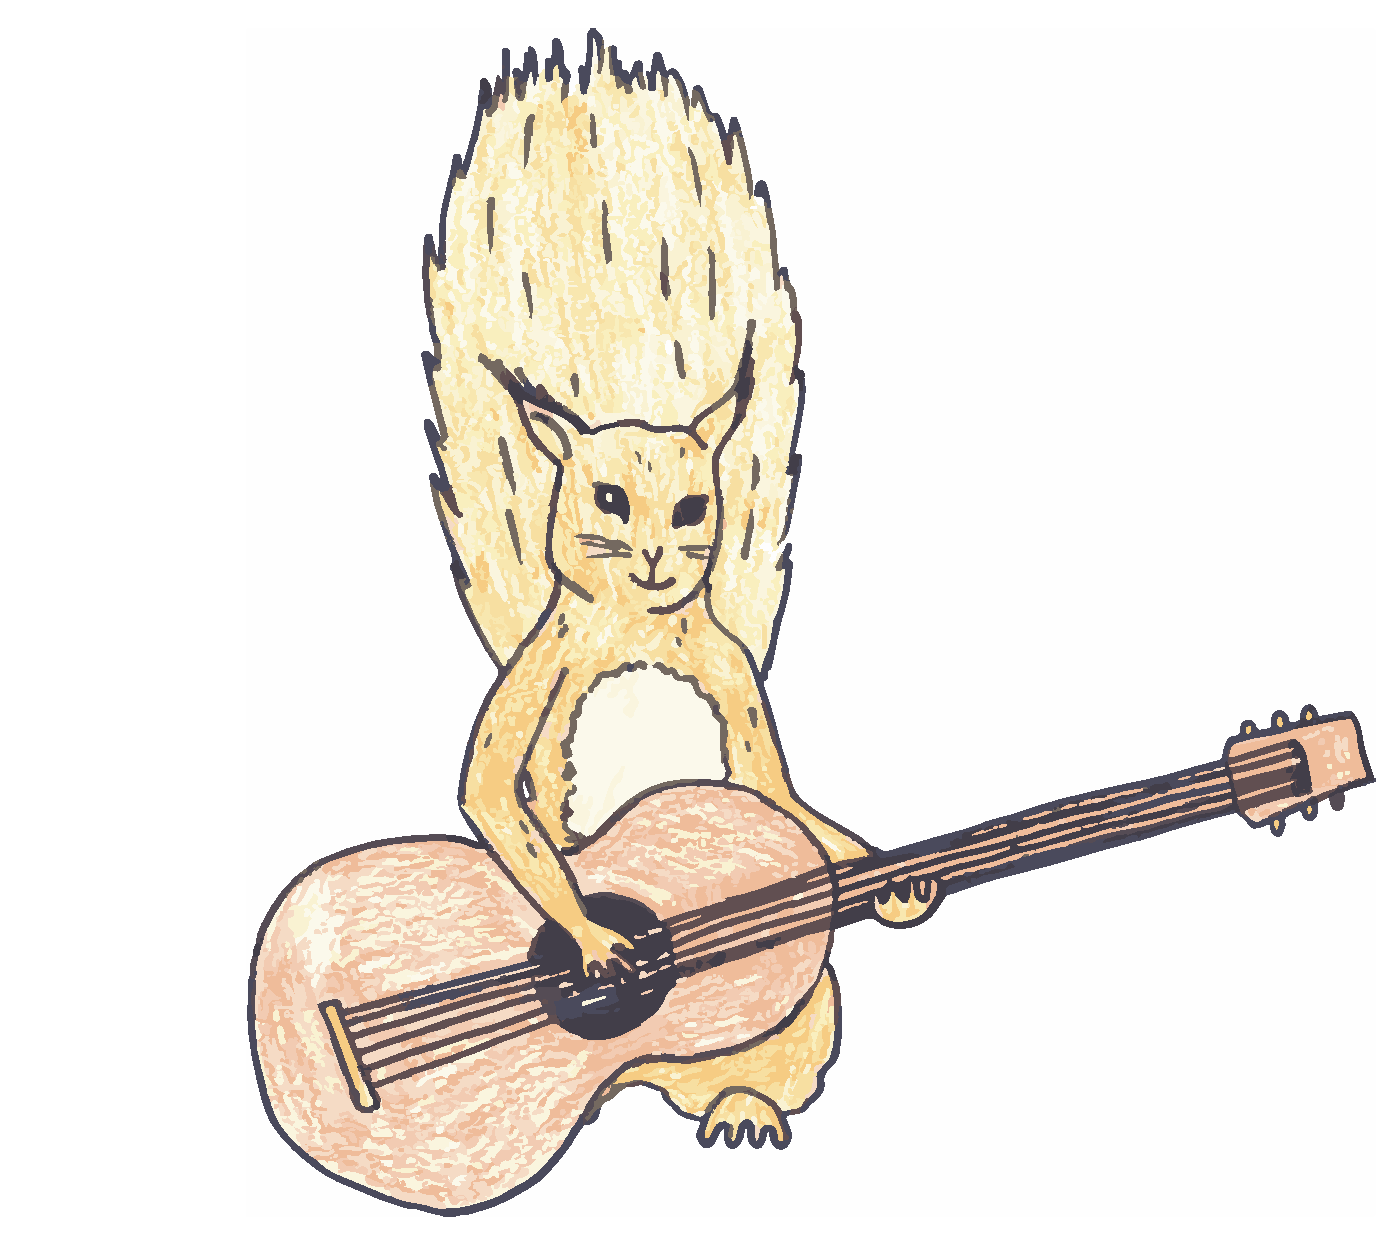
\includegraphics[scale=0.5]{veverka.pdf}\\
		\vspace{5em}
		{\fontsize{80}{90}\Fontskrivan\selectfont Zpěvník}
	\end{center}
	\end{figure}
\end{titlepage}


% První strana
\pagenumbering{gobble}
\noindent Tuto šablonu vytvořil \emph{VasaM} pod licencí Creative Commons (CC BY 4.0). Autorem původní šablony (\url{https://github.com/Vasek79/Kytarovy-zpevnik}) je \emph{Vasek79}. Texty s akordy jednotlivých skladeb a případné přílohy NEJSOU součástí této šablony a tudíž se na ně tato licence nevztahuje.\\
Dílo smíte:
\begin{itemize}
	\item \textit{sdílet} -- rozmnožovat a distribuovat materiál prostřednictvím jakéhokoli média v jakémkoli formátu
	\item \textit{upravit} -- remixovat, změnit a vyjít z původního díla pro jakýkoliv účel, a to i komerční.
\end{itemize}
Za podmínky uvedení jeho původu, tedy je Vaší povinností uvést autorství, poskytnout s dílem odkaz na licenci a vyznačit Vámi provedené změny. Toho můžete docílit jakýmkoli rozumným způsobem, nicméně nikdy ne způsobem naznačujícím, že by poskytovatel licence schvaloval nebo podporoval Vás nebo Váš způsob užití díla. Poskytovatel licence nemůže odvolat tato oprávnění do té doby, dokud dodržujete licenční podmínky.\\
\\
\\
Zdrojové soubory k tomuto zpěvníku najdete na \url{https://github.com/VasaMM/zpevnik}. Vytvořené pdf tamtéž.\\
\\
\\
\def\spotifyUrl{https://open.spotify.com/playlist/2eriz9vxG9uJzPwseSasVu?si=fcc7d09377ba4879}%
Ke zpěvníku byl vytvořen playlist pro službu Spotify \url{\spotifyUrl}.\\
\begin{center}
	\qrcode[nolink, height=3cm]{\spotifyUrl}
\end{center}
\vfill
\hfill\emph{Tento soubor byl vytvořen \today}.


% Obsah
\newpage
\tableofcontents
\thispagestyle{empty}

% Zapnu číslování stránek (jeli povoleno v konfiguraci)
\ifx\cislovaniStranekPovoleno\undefined
	% Cislovani je vyonuto, není nutné nic definovat
\else
	\pagenumbering{arabic}
	\setcounter{page}{0}
\fi

% Písničky
\addContentSection{A}
\hlavicka[Vlasta Redl]{A te Rehradice}

\sloka{
\Emi A te Rehradice \D na pěkný ro\G vině,\\
\A teče tam vo\Hmi děnka \Emi dole \A po dě\D dině,\\
\Ami je pěk\Hmi ná, je \Emi čistá.
}

\sloka{
A po tej voděnce drobný rebe skáčó,\\
pověz ně má milá, proč tvý voči pláčó\\
tak smutně, žalostně.
}

\sloka{
Pláčou oni, pláčou šohajó pro tebe,\\
že sme sa dostali daleko vod sebe,\\
daleko vod sebe.
}

\sloka{
Co by neplakaly, když hlavěnka bolí\\
musijó zaplakat šohajovi kvóli\\
šohajovi kvóli.
}

\hlavicka{Amazonka}{Hop Trop}

\sloka{
Byly krásný naše \A plány,\\
byla jsi můj celej \CisMi svět,\\
\Hmi čas je vzal a nechal \A rány,\\
sta\Hmi rší jsme jen o pár \E let.
}

\sloka{
Tenkrát byly děti malý,\\
ale život utíká,\\
už na "táto" slyší jinej,\\
i když si tak neříká.
}

\refren{
Nebe modrý zrcad\A lí se\\
v \FisMi řece, která všechno \Hmi ví,\\
stejnou barvu jako \A měly\\
t\Hmi voje oči džíno\E vý.
}

\sloka{
Kluci tenkrát, co tě znali, všude, kde jsem s tebou byl,\\
\uv{Amazonka} říkávali, a já hrdě přisvědčil.
}

\sloka{
Tvoje strachy, že ti mládí pod rukama utíká\\
vedly k tomu, že ti nikdo \uv{Amazonka} neříká.
}

\sloka{
Zlatý kráse cingrlátek, jak sis časem myslela,\\
vadil možná trampskej šátek, nosit dáls ho nechtěla.
}

\refren{
Teď jsi víla z paneláku, samá dečka, samej krám,\\
já si přál jen, abys byla pořád stejná, přísahám,\\
\Hmi pořád stejná, přísa\A hám.
}
\hlavicka{Anděl}{Karel Kryl}

\sloka{
\G Z rozmláce\Emi nýho kostela \G v krabici s \DSedm kusem mýdla\\
\G přinesl \Emi jsem si anděla, \G polámali \DSedm mu křídla,\\
\G díval se \Emi na mě oddaně, \G já měl jsem \DSedm trochu trému,\\
\G tak vtiskl \Emi jsem mu do dlaně \G lahvičku \DSedm od parfému.
}

\refren{
\G A proto, \Emi prosím, věř mi, \G chtěl jsem ho \DSedm žádat,\\
\G aby mi \Emi mezi dveřmi \G pomohl \DSedm hádat,\\
\G co mě čeká \EmiSiroky\DSedm a nemi\G ne,\\
\G co mě čeká \EmiSiroky\DSedm a nemi\G ne.
}

\sloka{
Pak hlídali jsme oblohu, pozorujíce ptáky,\\
debatujíce o Bohu a hraní na vojáky,\\
do tváře jsem mu neviděl, pokoušel se ji schovat,\\
to asi ptákům záviděl, že mohou poletovat.
}

\refren{}

\sloka{
Když novinky mi sděloval u okna do ložnice,\\
já křídla jsem mu ukoval z mosazný nábojnice,\\
a tak jsem pozbyl anděla, on oknem odletěl mi,\\
však přítel prý mi udělá novýho z mojí helmy.
}

\refren{}

\hlavicka{Až to se mnou sekne}{Jaromír Nohavica}
3/4 takt

\sloka{
\Ami Až obuju sirano \ESedm černe papirove \Ami boty,\quad\G\\
až i \C moja stara pocho\G pi, že nejdu do robo\C ty,\\
až \Dmi vyjde dluhy pruvod smutečnich hostu\\
na \Ami Slezsku Ostravu od Sykorova mostu,\\
\ESedm až to se mnu sekne, to bude \Ami pěkne,\\
\F pěkne, fajne a \Ami pěkne, \ESedm až to se mnu definitivně \Ami sekne.
}

\sloka{
Aby všeckym bylo jasne, že mě lidi měli radi,\\
ať je gulaš silny, baby smutne, muzika ať ladi,\\
bo jak sem nesnašel šledryjan ve vyrobě,\\
nebudu ho trpěť, ani co sem v hrobě,\\
to bude pěkne,\\
pěkne, fajne a pěkne, až to se mnu definitivně sekne.
}

\sloka{
S někerym to seka, že až neviš, co se robi,\\
jestli pomohla by deka nebo teplo mlade roby,\\
kdybych si moh vybrat, chtěl bych hned a honem,\\
ať to se mnu šlahne tajak se starym Magdonem,\\
to bude pěkne,\\
pěkne, fajne a pěkne, až to se mnu definitivně sekne.
}

\sloka{
Jedine, co nevim: jestli Startku nebo Spartu,\\
bo bych tam nahoře v nebi nerad trhal partu,\\
na každy pad s sebu beru bandasku s rumem,\\
bo rum nemuže uškodit, když pije se s rozumem,\\
to bude pěkne,\\
pěkne, fajne a pěkne, až to se mnu definitivně sekne.
}

\sloka{
Já vím, že, Bože, nejsi, ale kdybys třeba byl, tak\\
hoď mě na cimru, kde leži stary Lojza Miltag,\\
s Lojzu chodili sme do Orlove na zakladni školu,\\
farali sme dolu, tak už doklepem to spolu,\\
až to se mnu sekne,\\
pěkne, to bude pěkne, až to se mnu definitivně sekne.
}

\sloka{
Až obuju si rano černe papirove boty,\\
až i moja stara pochopi, že nejdu do roboty,\\
kdybych, co chtěl, dělal, všechno malo platne,\\
mohlo to byt horši, nebylo to špatne,\\
až to se mnu sekne,\\
k\F dybych, co chtěl, dělal, všechno malo platne,\\
m\Ami ohlo to byt horši, nebylo to špa\ESedm tne,\\
až to se mnu \dots\ na\F na na\dots \AmiSiroky\ESedmSiroky\AmiSiroky\FSiroky\AmiSiroky\ESedmSiroky\AmiSiroky
}

\addContentSection{B}
\hlavicka{Babička Mary}{Jan Werich, Jiří Voskovec}

\sloka{
\Ami Štěchovická \X laguna když dřímá \X v zadumaném stínu Kordy\X lér,\\
\Dmi pirát zkrva\Ami venou šerpu ždímá, \HSedm šerif si láduje revol\E ver.\\
\Ami Pikovická \X rýžoviště zlata \X čeří se v příboji Sáza\X vy,\\
\Dmi ale za to \Ami krčmářova chata \IDmi křepčí rykem \ESedm chlapské záb\IAmi avy.\\
\GSedm Když tu náhle, co se \C děje, \GSedm divný šelest houštím \C spěje,\\
\GSedm plch, skunk, \C vše utíká \IF po stráni \FisDim od Medn\IE íka.\\
\Ami Krčmář zhasne, \X kovbojové ztichnou, \X pirát zděšen tvář si zakry\X je,\\
\D rudé squaw se \Ami chvějí a pak vzdychnou:\\
\uv{\HSedm Blíží se k nám postrach préri\IE e}.\hspace{1em}\GSedm\hspace{1.5em}\I
}

\refrenX{1}{
\C Mary, \X babička \DSedm Mary, \X dva kolťá\GSedm ky za pasem,\\
\X nad hlavou \C točí lasem.\\
\X Stoletá \X Mary, \X babička \DSedm Mary, \X ta zkrotí \GSedm křepce hřebce,\\
\X ať chce či ne\IC chce.\ \ESedm\hspace{1.3em}\I
}

\sloka{
Žádné zuby, z jelenice sukně, ale za to tvrdé bicepsy,\\
Mary má vždy slivovici v putně, Toma Mixe strčí do kapsy.\\
Klika cvakla, v krčmě dveře letí a babička vchází do dveří,\\
\uv{Pintu ginu, lumpové prokletí!} bezzubou dásní zaláteří.\\
Vypiju to jen ve stoje, jdu do volebního boje,\\
zřím zas město drahý, jedu volit do Prahy.\\
Dopila a aby se neřeklo, putykáře změní v mrtvolu,\\
za zády má štěchovické peklo s šlajsnou svatojánských atolů.\\
}

\refrenX{2}{
Mary, babička Mary, pádluje bez námahy po proudu až do Prahy.\\
Stoletá Mary, babička Mary, jde do volebního boje za kovboje.\\
}
 
\sloka{
Ledva v Praze kotvu vyhodila, pro babičku nastal hrozný čas,\\
neboť hned každá strana tvrdila, že jí náleží babiččin hlas.\\
Malá stejně jako velká strana psala, že bude mít o hlas víc,\\
že ta druhá strana je nahraná, oni že maj hlas ze Štechovic.\\
Stoletý věk prý nevadí, na předáka je to mládí,\\
ze všech nejvíce, volala ji polnice.\\
Tak babičku, pro kterou vždy byla válka s lidojedy legrace,\\
tu babičku za pár dni zabila, volební agitace.\\
}


\refrenX{3}{
Mary, bojovná Mary, už nesedává v sedle, ve volbách byla vedle.\\
Stoletou Mary, babičku Mary, volbama zabitou vzal k sobě Manitou.\\
}
 
\hlavicka{Batalion}{Spirituál kvintet}

3/4 takt

\sloka{
\Ami Víno \C máš a \G marky\Ami tánku, \X dlouhá \C noc se \G prohý\Ami ří.\\
Víno máš a chvilku spánku, díky, díky verbíři.
}

\sloka{
\Ami Dříve, než se roze\X dní, kapitán \IC k osedlání \G rozkaz \IAmi dá\hspace{1.7em}\Emi vá,\quad\I\\
\Ami ostruhami do sla\IX bin   ko\G ně \IAmi po\hspace{1.7em}\Emi há\hspace{1.2em}\IAmi ní.\\
Tam na straně polední čekají ženy, zlaťáky a sláva,\\
do výstřelu karabin zvon už vyzvání.
}

\refren{
\Ami Víno na ku\C ráž a \G pomilovat marky\Ami tánku,\\
\Ami zítra do Bur\IC gund batalion\IAmi\ za\hspace{1.5em}\Emi mí\hspace{1.3em}\IAmi ří.\\
Víno na kuráž a k ránu dvě hodinky spánku,\\
díky, díky vám královští verbíři.
}

\sloka{
Rozprášen je batalion, poslední vojáci se k zemi hroutí,\\
na polštáři z kopretin budou věčně spát.\\
Neplač sladká Marion, verbíři nové chlapce přivedou ti,\\
za královský hermelín padne každý rád.
}

\refren{}

\slokaOpakovani{1.}{}
 \hlavicka[bratři Ryvolové]{Bedna od whisky}

\sloka{
\Ami Dneska už mě \C fóry ňák \Ami nejdou přes \E pysky \\
\Ami Stojím s dlouhou \C kravatou na \IAmi bedně \E vod wh\IAmi isky. \\
Stojím s dlouhým \C vobojkem jak \Ami stájovej \E pinč. \\
\Ami Tu kravatu \C co nosím mi \IAmi navlík \E soudce\IAmi\ Linč.\quad\X
}

\refren{
\A Tak \X kopni do tý \D bedny ať \E panstvo neče\A ká \\
jsou \X dlouhý schody do \D nebe a \E štreka dale\A ká. \\
Do \X nebeskýho \D báru já \E sucho v krku \A mám. \\
Tak \X kopni do tý \D bedny ať \E na cestu se \A dám.\ hspace{1em}\XSiroky\XSiroky\XSiroky
}

\sloka{
Mít tak všechny bedny od whisky vypitý. \\
Postavil bych malej dům na louce ukrytý. \\
Postavil bych malej dům a z okna koukal ven \\
a chlastal bych tam s Billem a chlastal by tam Ben.
}

\refren{}

\sloka{
Kdyby si se hochu jen pořád nechtěl rvát. \\
Nemusel jsi dneska na týhle bedně stát. \\
Moh si někde v suchu tu svoji whisky pít\\
nemusel si hochu na krku laso mít.
}

\refren{}

\sloka{
Když jsem štípnul koně a ujel jen pár mil\\
nechtěl běžet dokavád se whisky nenapil\\
zatracená smůla zlá a zatracenej pech\\
když kůň cucá whisku jak u potoka mech.
}

\refren{}

\sloka{
Až kopneš do tý bedny, jak se to dělává \\
do krku ti zůstane jen dírka mrňavá. \\
Jenom dírka mrňavá a k smrti jenom krok. \\
mám to smutnej konec - a whisky ani lok
}

\refren{Tak kopni do tý bedny ať panstvo nečeká \\
jsou dlouhý schody do nebe a štreka daleká. \\
Do nebeskýho báru já sucho v krku mám\\
tak kopni do tý bedny!}
\zvyraznit
\takt{6}{8}
\hlavicka[Pavel Dydovič]{Bláznova ukolébavka}

\sloka{
\G Máš má ovečko \D dávno spát, i \C píseň ptáků \G končí,\\
\X kvůli nám přestal \D vítr vát, jen \C můra zírá \G zvenčí\\
Já \D znám její zášť tak \C vyhledej skrýš,\\
zas \D má bílej plášť a \IC v okně je \D mříž\I .
}

\refren{
\G Máš má ovečko \D dávno spát\\
a \C můžeš hřát ty mně \A můžeš hřát\\
Vždyť \G přijdou se \C ptát,\\
zítra zas \G přijdou se \C ptát\\
jestli ty v \G mých předsta\C vách už \G mizíš.
}

\sloka{
Máš má ovečko dávno spát, dnes máme půlnoc temnou.\\
Ráno budou nám bláznům lát, že ráda snídáš se mnou.\\
Proč měl bych jim lhát že jsem tady sám,\\
když tebe tu mám když tebe mám rád.
}
\hlavicka[Greenhorns]{Blues Folsomské věznice}

\sloka{
\G Můj \X děda bejval \X blázen, te\X xaskej Ahas\X ver,\\
a \X na půdě nám \X po něm zůstal \GSedm ošoupanej \X kvér.\\
Ten \C kvér obdi\X vovali všich\X ni kámoši \X z oko\G lí\\
a \D máma mi ří\X kala: „\X Nehraj si s tou \DSedm pisto\G lí!“
}

\sloka{
Jenže i já byl blázen tak zralej pro malér\\
a ze zdi jsem sundával tenhle ten dědečkův kvér.\\
Pak s kapsou vyboulenou chtěl jsem bejt chlap \uv{All right}\\
a s holkou vykutálenou hrál jsem si na Boonie and Clyde.
}

\sloka{
Ale udělat banku, to není žádnej žert,\\
sotva jsem do ní vlítnul hned zas vylít' jsem jak čert.\\
Místo jako kočka já utíkám jak slon,\\
takže za chvíli mě veze policejní anton.
}

\sloka{
Teď okno mřížovaný mně říká, že je šlus,\\
proto tu ve věznici zpívám tohle Folso blues.\\
Pravdu měla máma, radila: Nechoď s tou holkou!\\
a taky mně říkala: Nehraj si s tou pistolkou!
}

\hlavicka{Blues na cestu poslední}{Semafor}

\sloka{
\D Černej nebožtíku, \GSedm máš to ale kliku,\\
\D za chvíli do temný hlíny \DSedm budeš zakopán,\\
\GSedm Černej nebožtíku, \X máš to ale kliku,\\
\D za chvíli do temný hlíny \X budeš zakopán,\\
\ASedm nás jsi nechal v bídě, \GSedm sám se vezeš jako \D pán.
\FisDim\hspace{4em}\Fdim\hspace{3.5em}\D\hspace{2em}\DisDim\hspace{4.2em}\ASedm
} 

\sloka{
Jen kopyta koní hrany tobě zvoní,\\
málo lidí dnes pro tebe slzy polyká,\\
je to smutnej funus, chybí ti tu muzika.
}

\sloka{
Kam ti pozůstalí, kam ti vlastně dali\\
věnce, kytky, pentle, svíce, marně se ptám,\\
proč je rakev holá, to ty asi nevíš sám.
}

\sloka{
Černej nebožtíku, když nemáš na muziku,\\
poslechni mou radu trochu nevšední,\\
zazpívej si sám blues na cestu poslední.
}

\hlavicka[Petr Kalandra]{Břímě}

\sloka{
\G Včera mě spolkl \Hmi Nazareth, aby \C dnes vypliv ostatky \G mý\\
celou noc hledám místo kam složit vlasy šedivý\\
hej pane nechcete mi říct, kde tu můžu složit hlavu svou\\
né řekl a hned zmizel tam za tou velkou bílou budovou.
}

\refren{
\G Sundej \Hmi z něj to \C břímě \G a nechtěj \Hmi za to \C nic\\
\G dědek ať \Hmi už se \C nedře, hej, hej, héééj \\
nandej mi ho na zá\G da.\HmiSiroky\CSiroky\GSiroky\DSiroky\EmiSiroky\DSiroky\CSiroky
}

\sloka{
Přes rameno ranec svůj, jak rád bych nějaký místo měl\\
kam bych se v klidu schoval a na všechno bych zapomněl\\
v tom vidím Carmen s Ghiou jak po ulici proti jdou\\
Carmen že nemá čas, že si spolu rychle užijou.
}

\refren{
Sundej z nich to břímě a nechtěj za to nic holky ať už se nedřou\dots
}

\sloka{
Když přijdeš k paní Mósrové, tak tam není co bys řek\\
připadáš si jak v automatu ve frontě na párek\\
povídá: \uv{Mladej kmete, a což takhle třeba Nathalii?}\\
už není právě nejmladší a tak zůstaň dneska večer s ní.
}

\refren{
Sundej z ní to břímě a nechtěj za to nic holka ať už se nedře\dots
}

\sloka{
Postarší právník mě nakop a to rovnou do koulí\\
povídá já ti cestu ukážu ale musíš s mým psem ven\\
povídám moment soudče já jsem taky Homo sapiens\\
Abych si trochu ulehčil tu ránu jsem mu navrátil.
}

\refren{
Sundej z něj to břímě a nechtěj za to nic dědek ať už se nedře\dots
}

\sloka{
Na dělový kouli z roku 1835 se vezu někam dolů,\\
je načase mi závidět.\\
Tak letím mezi vás, pozdravuje vás tamten svět\\
že prej se nemusíte vracet, je načase mi závidět
}

\refren{
Sundej ze mě to břímě a nechtěj za to nic ať už se nikdy nedřu\dots nandej si ho na záda.
}

\hlavicka[Michal Tučný]{Buráky}

\sloka{
Když \D Sever válčí s Jihem \IG a zem jde do vá\D lky, na\I\\
\X polích místo bavlny te\IE ď rostou bodláky.\ASedm Ve\ \I\\
\D stínu u silnice vidí\IG m z Jihu vojá\D ky, jak\I\\
\X válejí se líně \IASedm a louskaj burá\D ky.\ \I
}

\refren{
Hej \D hou, hej hou, na\IG č chodit do vá\D lky, je\I\\
\X lepší doma sedět \IE a louskat bur\ASedm áky. Hej\I\\
\D hou, hej hou, na\IG č chodit do vá\D lky, je\I\\
\X lepší dom\IASedm a sedět a louskat burá\D ky.\I
}

\sloka{
Plukovník je v sedle, volá: \uv{Yankeeové jdou!},\\
ale mužstvo v trávě leží, prej dál už nemohou,\\
plukovník se otočí a koukne do dálky,\\
tam jeho slavná armáda teď louská buráky.
}

\refren{}

\sloka{
Až tahle válka skončí a my zas budem žít,\\
svý milenky a ženy pak půjdem políbit,\\
Když se zeptaj: \uv{Hrdino, cos dělal za války?}\\
\uv{Já flákal jsem se s kvérem a louskal buráky.}
}

\refren{}
\addContentSection{C}
\hlavicka{Cesta}{Kryštof}

\sloka{
Tou \C cestou,
tím směrem prý, bych se dávno měl \G dát.\\
Když \Ami sněží, jde to stěží, ale sněhy pak tají.\\
Kus \F něhy ti za nehty \G slíbí a dají.  \\
Víc síly se prát, na dně víc dávat než brát.\\
A i když se vleče a je schůdná jen v kleče,\\
donutí přestat se zbytečně ptát.
}

\refren{
Jestli se \C blížím k cíli,\\
kolik \G zbývá víry, kam \Ami zvou\\
svodidla, co po tmě mi \F lžou?\ \G\\
Zda couvám zpátky\\
a plýtvám řádky, co řvou,\\
že už mi doma neotevřou .
}

\sloka{
Nebo jít s proudem,\\
na lusknutí prstu se začít hned smát.\\
Mít svůj chodník slávy a před sebou davy\\
a přes zkroucená záda být součástí stáda.\\
Ale zpívat a hrát, kotníky líbat, a stát,\\
na křídlech všech slavíků, a vlastně už ze zvyku,\\
přestat se zbytečně ptát.
}

\refren{}
\refren{}

\zvyraznit
\hlavicka[Vypsaná fiXa]{Čtyři slunce}

\slokaBezCisla{
\IEmi\qquad\quad\CSiroky\IG\qquad\D\quad\I\quad\akord{$2\times$}
\vspace{-1em}
}

\sloka{
\IEmi Čtyři \C slunce \IG svítěj p\D ro radost,\I\quad \EmiSiroky\CSiroky\IG\qquad\DSiroky\I \\
\IEmi vlnovk\C a se z\IG vedne, \D když má dost.\I\quad  \EmiSiroky\CSiroky\IG\qquad\DSiroky\I \\
A \Emi čtyři slunce \C svítěj,\\
li\Ami dem pod nima \D není zima.\\
Si \Emi jako malý \C dítě\\
a \Ami můžes začít \D zase znova.
}

\refren{
Já \Emi vím,\C\ někdy to \Ami nejde.\ID\qquad\DsusCtyri\qquad\quad\I \\
Já \Emi vím,\C\ všechno to \Ami přejde.\ID\qquad\DsusCtyri\qquad\quad\I
}

\slokaBezCisla{
\IEmi\qquad\quad\CSiroky\IG\qquad\D\quad\I\quad\akord{$2\times$}
\vspace{-1em}
}

\sloka{
Čtyři slunce svítěj pro radost,\\
přejdu řeku, vede přes ní most.\\
Čtyři slunce svítěj,\\
lidem pod nima není zima.\\
Si jako malý dítě\\
a můžes začít zase znova.
}

\refren{}

\slokaOpakovani{1.}{}

\refren{}
\refren{}

\sloka{
Čtyři slunce svítěj pro radost,\\
vlnovka se zvedne, když máš dost.
}

\hlavicka{Čůrej!}{Kašpárek v rohlíku}

\slokaBezCisla{\DSiroky\GSiroky\DSiroky\hspace{1em}\DSiroky\GSiroky\DSiroky}

\sloka{
Čůrej sem a čůrej tam,\DSiroky\GSiroky\DSiroky\\
čůrej jako velkej pán.\DSiroky\GSiroky\DSiroky\\
Ve stoje i za běhu,\GSiroky\FSiroky\GSiroky\\
žlutý srdce do sněhu.\DSiroky\GSiroky\DSiroky\\
Každej se rád vyčůrá,\ASiroky\ASedmSiroky\\
zadara i za bůra.\DSiroky\GSiroky\DSiroky
}

\sloka{
Čůrej sem, sem, sem,\\
čůrej dovnitř, čůrej ven,\\
řekni mi kam čůrat mám,\\
já se ti tam vyčůrám.\\
Ať jsi s partou nebo sám,\\
čůrej sem a čůrej tam.
}

\refren{
Ať seš velkej nebo \D malej,\GSiroky\DSiroky\\
do sklenice vodu \D nalej,\GSiroky\DSiroky\\
ten kdo hodně vody \G lemtá,\FSiroky\GSiroky\\
přečůrá i \D prezidenta.\GSiroky\DSiroky\\
A když nevíš kudy \D kam,\GSiroky\DSiroky\ASiroky
}

\sloka{
3. Čůrej doma, čůrej v metru, (hlavně rychle ještě dneska)\\
jen nečůrej proti větru! (skvělej výkon všichi tleskaj)\\
Malí ještě nevinný, (můžou čůrat do plíny)\\
maj to pěkně s rámusem. \\
Ať jsi s partou nebo sám, (holky se maj můžou sedět)\\
čůrej sem a čůrej tam. (holky se maj můžou sedět)
}

\refren{}

\sloka{
Čůraj Češi, čůraj Němci,\\
hrozně tupí vytlemenci,\\
někdy kýbl, někdy deci.\\
Na dnešek mám dobrej plán.\\
Čůrat sem a čůrat tam\A .
}

\addContentSection{D}
\zvyraznit
\hlavicka[Olympic]{Dej mi víc své lásky}

\sloka{
\EmiSiroky\GSiroky\EmiSiroky\DSiroky\HSedmSiroky\\
\Emi Vymyslel jsem \X spoustu nápa\X dů, a\G -ú,\\
co \Emi podporujou \X dobrou nála\D du, a\HSedm -ú,\\
\Emi hodit klíče \X do kanálu, \A sjet po zadku \Ami holou skálu,\\
\Emi v noci chodit \HSedm strašit do hra\Emi du.\qquad\X
}

\sloka{
Dám si dvoje housle pod bradu, a-ú,\\
v bíle plachtě chodím pozadu, a-ú,\\
úplně melancholicky, s citem pro věc, jako vždycky,\\
vyrábím tu hradní záhadu.\quad\DSedm
}

\refren{
\G\quad Má drahá \X dej mi víc,\HSedm\quad má drahá \X dej mi víc,\\
\Emi\quad má drahá \C dej mi víc své \G lásky, a\DSedm -ú,\\
\G\quad já nechci \X skoro nic,\HSedm\quad já nechci \X skoro nic,\\
\Emi\quad já chci jen \C pohladit tvé \G vlásky, a\HSedm -ú.
}

\sloka{
Nejlepší z těch divnej nápadů, a-ú,\\
mi dokonale zvednul náladu, a-ú,\\
natrhám ti sedmikrásky,\\
tebe celou s tvými vlásky\\
zamknu si na sedm západů, a-ú.
}

\slokaBezCisla{
\EmiSiroky\EmiSiroky\EmiSiroky\GSiroky\EmiSiroky\EmiSiroky\DSiroky\HSedmSiroky\EmiSiroky\EmiSiroky\ASiroky\AmiSiroky\EmiSiroky\HSedmSiroky\EmiSiroky\DSedmSiroky
}

\refren{}
\vspace{-1em}

\slokaOpakovani{3.}{
\dots zamknu si na sedm západů, a-ú, \Emi aú, aú, aú, \E aú.
}
\zvyraznit
\hlavicka[Vypsaná fiXa]{Dezolát}

\sloka{
\Emi Ty si pěkný \C dezolát \D řekla \uv{Halí\AsusDva belí}\\
a byla to \Emi pohoda třeba se to \C povede\\
\D vytáhnem tvý \AsusDva múzy a hodíme je \Emi za tebe\\
kdo ty múzy \C zachytí \D ten bude mít \AsusDva záruku\\
opravdový \Emi kvality ty si pěkný \C dezolát\\
\D tohle řekla \AsusDva ona musíme tě \C sledovat.
}

\refren{
A celý \Emi prostor\\
je sledova\C ný\\
příjemnými \Emi lidmi kteří olizu\C jí\\
šťávu \Emi tekoucí\\
z konečků \D prstů.\DsusCtyriSiroky\DSiroky
}

\sloka{
\Emi Ty jsi pěkný \C dezolát \D ve sprchovým \AsusDva koutě\\
teče voda \Emi ledová třeba se to \C povede\\
\D opláchnu svý \AsusDva múzy a vypustím je \Emi pod sebe\\
kdo ty múzy \C zachytí \D ten bude mít \AsusDva záruku\\
opravdový \Emi kvality a ty si pěkný \C dezolát\\
\Dtohle řekla \AsusDva ona.
}

\refren{}


\sloka{
\Emi Pustíme si \C starý gramo\D fon\\
budeme mít \AsusDva světy\\
který nás zajíma\Emi jí\\
vinylový \C bůh je šampi\D on\\
proležíme \AsusDva v posteli\\
celou nedě\Emi li\\
pustíme si \C starý gramo\D fon\\
budeme mít \AsusDva světy\\
který nás zajíma\Emi jí\\
vinylový \C bůh je šampi\D ón\\
venku ten \AsusDva náš svět\\
sledují kame\Emi ry\\
\C A hudba hraje \D dál,\\
\AsusDva sledují kame\Emi ry.\\
\C A hudba hraje \D dál.\AsusDvaSiroky\\
\Emi Pustíme si \C starý gramo\D fon.\AsusDvaSiroky\\
\Emi Pustíme si \C starý gramo\D fon.\AsusDvaSiroky
}

\sloka{
\Emi pustíme si \C starý gramo\D fon\\
budeme mít \AsusDva světy\\
který nás zajíma\Emi jí\\
vinylový \C bůh je šampi\D ón\\
venku ten \AsusDva náš svět\\
sledují kame\Emi ry.
}

\sloka{
\Emi Jsem \C z toho celej \D žhavej.
}

\begin{center}
	~~\hmatAsusDva~~\hmatDsusCtyri~~
\end{center}
\hlavicka[Petr Kalandra]{Dětské šaty}


\sloka{
\EmiSiroky\CSiroky\DSiroky\GSiroky\EmiSiroky\CSiroky\DSiroky\GSiroky\\
\Emi Setři si \C tvář \D a slzí \G pár\\
\Emi a neplač \C co ti na nich \D zále\G ží.\\
\Emi Dnes přišla \C chvíle a \D mě se zdá,\G\\
\Emi že dětské šaty jsou ti \G přítěží \C čas je odnáší,\G\\
\Emi že dětské šaty jsou ti \G přítěží \C čas je odnáší.\G
}

\sloka{
\EmiSiroky\CSiroky\DSiroky\GSiroky\EmiSiroky\CSiroky\DSiroky\GSiroky\\
Šli jsme loukou, šli jsme strání\\
a dětství odletělo bůhví kam.\\
Má pestrost křídel a dívčích přání\\
a nebo jako kytka uvadá v nočních zahradách\\
a nebo jako kytka uvadá v nočních zahradách.

}

\refren{
\Emi Dětství odletělo \D bůhví \Emi kam\\
\Emi zpátky nevrátí se, \D já ho \Emi znám.\\
Dětství odletělo bůhví kam\\
zpátky nevrátí se, já ho znám, \C nevěř pohádkám.\G
}

\hlavicka[Jaromír Nohavica]{Divocí koně}

\sloka{
\repetice{\Ami Já viděl \IDmi divoké \Ami koně,\IC\ běželi \Dmi soumrakem\IAmi ,}
\IDmi vzduch \Ami těžký\I\ \IDmi byl a divně \Ami voněl \IDmi tabá\quad\F kem,\\
\IDmi vzduch \Ami těžký\I\ \IDmi byl a divně \Ami voněl \ESedm tabá\IAmi kem.
}

\sloka{
\repetice{Běželi, běželi bez uzdy a sedla krajinou řek a hor,}
\repetice{sper to čert, jaká touha je to vedla za obzor?}
}

\sloka{
\repetice{Snad vesmír nad vesmírem, snad lístek na věčnost,}
\repetice{naše touho, ještě neumírej, sil máme dost.}
}

\sloka{
\repetice{V nozdrách sládne zápach klisen na břehu jezera,}
\repetice{milování je divoká píseň večera.}
}

\sloka{
\repetice{Stébla trávy sklání hlavu, staví se do šiku,}
\repetice{král s dvořany přijíždí na popravu zbojníků.}
}

\sloka{
\repetice{Chtěl bych jak divoký kůň běžet, běžet, nemyslet na návrat,}
\repetice{s koňskými handlíři vyrazit dveře, to bych rád.}
Já viděl divoké koně\dots
}

\zvyraznit
\hlavicka[Chinaski]{Dobrák od kosti}

\sloka{
\D Má milá \A jak ti je, tak \G jak ti je?\ \X\\
\D Jsem ten, kdo \A jednou tvý \G tělo zakryje.\ \CaddDevet\\
Jsem ten, kdo tě jednou oddělá.\\
Potkala's zkrátka koho's neměla.
}

\sloka{
\DSiroky\ASiroky\GSiroky\GSiroky\\
Jsi budoucí krev v mojí posteli.\\
Jsem ten, kdo tě jednou jistojistě zastřelí.\\
Jsem ten kdo ty tvoje krásný oči jednou zatlačí.\\
Jsi moje všechno a mě to nestačí.
}

\refren{
\D Je to vážně silná \X káva, \A pláč a nebo \X vztek \G nic už s tím \X nenaděláš,\\
\D nech mě jenom \X hádat, \A jak jsi hebká na \X dotek \G krásná a \X nedospělá.
}

\sloka{
Víš, všechno má aspoň malý kaz,\\
jsem ten, kdo ti jednou zlomí vaz.\\
Má milá vždyť mě znáš jsem dobrák od kosti,\\
a ty jsi ta co mi to jednou všechno odpustí.
}

\sloka{
\D Sejde z očí \X sejde z mysli,\\
\A jenom blázen věří \X na nesmysly,\\
\G láska je čaroděj \X a ticho prý léčí,\\
\X ale zákon hovoří \X jasnou řečí.
}

\refren{}

\slokaBezCisla{
\D Má milá \A jak ti je, tak \G jak ti je?\ \X\\
\D Jsem ten, kdo \A jednou tvý \G tělo zakryje.\ \CaddDevet
}

\vspace{-25em}
\noindent\hspace*{27em}\hmat[]{p3,p2,n,n,p3,p3}{\akordhmat{G}}\\
\\\\
\noindent\hspace*{27em}\hmatCaddDevet


\hlavicka{Dokud se zpívá}{Jaromír Nohavica}

3/4 takt

\sloka{
\C Z Těšína \Emi vyjíždí \DmiSedm vlaky co \F čtvrthodi\C nu,\quad\EmiSiroky\DmiSedmSiroky\GSedmSiroky\\
\C včera jsem \Emi nespal a \DmiSedm ani dnes \F nespoči\C nu,\quad\EmiSiroky\DmiSedmSiroky\GSedmSiroky\\\F 
\F svatý Med\G ard, můj pa\C tron, ťuká \IC si na \Ami če\hspace{1.3em}\IG lo,\quad\G\\
\F ale dokud se \G zpívá, \F ještě se \G neumře\C lo, \Emi hó\hspace{1.2em}\DmiSedm hó.\hspace{1.5em}\GSedm
}

\sloka{
Ve stánku koupím si housku a slané tyčky,\\
srdce mám pro lásku a hlavu pro písničky,\\
ze školy dobře vím, co by se dělat mělo,\\
ale dokud se zpívá, ještě se neumřelo, hóhó.
}

\sloka{
Do alba jízdenek lepím si další jednu,\\
vyjel jsem před chvílí, konec je v nedohlednu,\\
za oknem míhá se život jak leporelo,\\
ale dokud se zpívá, ještě se neumřelo, hóhó.
}

\sloka{
Stokrát jsem prohloupil a stokrát platil draze,\\
houpe to, houpe to na housenkové dráze,\\
i kdyby supi se slítali na mé tělo,\\
tak dokud se zpívá, ještě se neumřelo.
}

\sloka{
Z Těšína vyjíždí vlaky až na kraj světa,\\
zvedl jsem telefon a ptám se: \uv{Lidi, jste tam?}\\
A z veliké dálky do uší mi zaznělo,\\
že dokud se zpívá, ještě se neumřelo.\\
Že dokud se zpívá ještě se neumřelo.
}


\zvyraznit
\hlavicka[Chinaski]{Drobná paralela}

\slokaBezCisla{
\CSiroky\GSiroky\DSiroky\DSiroky\akord{$4\times$}
\vspace{-1em}
}

\sloka{
Ta \C stará \G dobrá hra je \D okoukaná.\quad\X\\
\C\quad Nediv se brá\G cho, kdekdo ji \D zná.\quad\X\\
\C\quad Přestaň se ptát:\G\ \uv{bylo nebylo líp?\D}.\quad\X\\
\C\quad Včera je vče\G ra, bohužel bohudík.\D\quad\X
}

\refren{
\C Nic není jako \G dřív,\quad\D nic není jak \Emi bejvávalo.\\
\C Nic není jako \G dřív,\quad\D to se nám to \Emi mívávalo.\\
\C Nic není jako \G dřív,\quad\D ačkoliv máš všechno \Emi co jsi vždycky chtěla.\\
\C Nic není jako \G dřív,\quad\D ačkoliv drobná para\Emi lela by tu byla.
}

\sloka{
\C Snad nevěříš \G na tajný znamení\D.\quad\X\\
\C Všechno to harampádí, \G balábile, \D mámení\quad\X\\
\C Vážení platící, \G jak všeobecně \D ví se,\quad\X\\
\C včera i dneska, \G stále ta samá \D píseň.\quad\X\quad Ačkoli
}

\refren{}

\slokaBezCisla{
\CSiroky\GSiroky\DSiroky\DSiroky\akord{$3\times$}
}

\sloka{
\C Promlouvám k vám \G ústy múzy, \D vzývám tón a \Emi lehkou chůzi,\\
\C vzývám zítřek \G nenadálý, \D odplouvám a \Emi mizím.\quad\X
}

\refren{
\C Nic není jako \G dřív,\quad\D nic není jak \Emi bejvávalo.\\
\C Nic není jako \G dřív,\quad jó, \D to se nám to dlouze \Emi kouřívalo.\\
\C Bohužel bohu\G dík je s námi, \D ta nenahmatatelná \Emi intimita těla.\\
\C Nic není jako \G dřív, jen fámy,\quad \D bla, bla, \Emi bla, bla et cetera.\\
\C Nic není jako \G dřív, \D nic není jak \Emi bejvávalo,\\
\C bohužel bohu\G dík,\quad \D co myslíš ségra, je to \Emi hodně nebo máloooo\C ooo\\
oo\G oooo o\D ooooo o\Emi oooo?\\
\CSiroky\GSiroky\DSiroky\EmiSiroky\akord{$2\times$}
}
\zvyraznit
\hlavicka[Chinaksi]{Duše z gumy}

\slokaBezCisla{
\GSiroky\DSiroky\EmiSiroky\CmajSedmSiroky\akord{$2\times$}
}

\sloka{
Mám duši \G gumovou a srdce \D ze železa \\
ale když \AmiSedm zavoní mi tvoje \C kombinéza\\
duše se \G vzedme a srdce \D zabuší\\
modravý \AmiSedm obláček zavoní \C ovzduším.\\
Kola se protočí, letíme vpřed\\
patníky lížem, jsou sladké jak med\\
a večer po šichtě jemine panečku\\
všichni tam společně hodíme zpátečku.
}

\refren{
\repetice{\G Mám duši z gumy a \D boky plechový\\
jsem \Emi jenom dopravní pros\CmajSedm tředek kolový\\
\G Mám duši z gumy a \D srdce z ocele\\
přesto ho \AmiSedm miluji, řidiče \CmajSedm přítele.}
}

\sloka{
Vždyť jenom pro tebe můj pane řidiči\\
buší mi motor a vře voda v chladiči\\
vždyť jenom pro tebe, ach, ty můj motorů světe\\
blinkry mi blikají a blatník mi kvete.\\
Po vlídném doteku šoféra prahnu\\
kdykoli bude chtít, vždycky mu zahnu\\
a večer po šichtě jemine panečku\\
společně hodíme zpátečku.
}

\refren{}

\sloka{
\G Až jednou za \D mnoho dní\\
\Emi na kilometru \X posledním\\
já \G hrdě vypustím svou \D duši\\
dík \C žes vždycky jel tak, jak \X se sluší.\\
Až jednou za mnoho dní\\
naposled motor zavrní\\
děkuji, že na naší trase\\
jels jako pán a ne jako prase.
}

\refren{}

\slokaBezCisla{
\G Máááá\D ám duši z \Emi gumy \CmajSedm (Společně hodíme zpátečku).\\
\G Máááá\D ám srdce z \AmiSedm ocele \CmajSedm (Řidiče přítele).\\
\G Máááá\D ám duši z \Emi gumy \CmajSedm (Společně hodíme zpátečku).\\
\G Máááá\D ám srdce z \AmiSedm ocele.\CmajSedmSiroky\GSiroky
}

\begin{center}
	~~\hmatCmajSedm~~
\end{center}
\hlavicka{Ďábel a syn}{Kabát}

\sloka{
\Dmi Sedím a koukám jak \C zvrácenej podzim\\
\Ami stromům svlíká jejich \G šat\\
\Dmi poslouchám ptáky a \C jenom tak kouřím\\ 
\Ami malinko chce se mi \G spát\\\\ 
Padá mi hlava pak cejtím jak někdo\\ 
lehce mě za ruku vzal\\
blázen či voják jak maškara divná\\ 
tam \Ami stál já pozval ho \Dmi dál\
}


\sloka{
Měl špinavej kabát a v ruce flétnu\\
oči jak z mrtvejch by vstal\\
na botách bahno snad celýho světa\\ 
a tuhletu píseň mi hrál\\\\
Tu píseň co zpívám a vůbec vám nevím\\ 
kde na ni akordy vzal\\
jak sem tam seděl a koukal a kouřil\\ 
to já teprv ji psal 
}

\sloka{
Povídá hochu vracim se z flámu\\ 
hráli jsme karty se zdá\\
partii pokera o budoucí vládu\\
dík bohu vyhrál jsem já\\\\
Já měl z pekla štěstí a nebo pár trumfů\\ 
v rukávu podvod - já vím\\
chcete mě soudit tak dejte mě na kříž\\ 
jsem váš ďábel a syn
}

\sloka{
Pak pomalu mluvil a ničil mě silou\\
co od věků v sobě už má\\
drtil mě pravdou a pouštěl mi žilou\\
na závěr jen povídá\\\\
Bůh stvořil lásku a žal taky bolest\\
a já jenom ubohej chtíč\\
fandím vám lidem nevím proč nemáš\\
mě rád já poslal ho pryč
}

\sloka{
Sedím a koukám jak zvrácenej podzim\\ 
stromům svlíká jejich šat\\
poslouchám ptáky a jenom tak kouřim\\
a malinko chce se mi spát\\\\
Padá mi hlava pak cejtim jak někdo\\ 
lehce mě za ruku vzal\\
blázen či voják jak maškara divná\\ 
tam stál tak pozvem ho dál
}

\addContentSection{F}
\hlavicka[Nedvědi]{Franky Dlouhán}

\sloka{
Kolik je \C smutného když \F mraky černé \C jdou\\
\X lidem nad hlavou \GSiroky\F smutnou dála\C vou\\
\X\quad já slyšel \X příběh, který \F velkou pravdu \C měl\\
\X za čas odletěl, \GSedmSiroky\F každý zapo\C mněl
}

\refren{
\C Měl kapsu \GSedm prázdnou Franky \X Dlouhán \\
po státech \F toulal se jen \C sám\\
a že byl \F veselej tak \C každej měl ho \GSedm rád\\
\GSedm  tam ruce \F k dílu mlčky \X přiloží\\
a \C zase jede \Ami dál a \F každej, \\
kdo s ním \GSedm chvilku byl, tak \IF dlouho \GSedm se pak smál\IC .\hspace{2em}\X
}

\sloka{
Tam, kde byl pláč, tam Franky hezkou píseň měl \\
slzy neměl rád, chtěl se jenom smát\\
a když pak večer ranče tiše usínaj\\
Frankův zpěv jde dál nocí s písní dál.
}

\refren{}

\sloka{
Tak Frankyho vám jednou našli přestal žít, \\
jeho srdce spí tiše smutně spí\\
Bůhví a za co tenhle smíšek konec měl \\
farář píseň pěl umíráček zněl.
}

\refren{}

\addContentSection{G}
\takt{2}{4}
\hlavicka[Čechomor]{Gorale}

\sloka{
\D Za lasami za \G gorami \A za dolina\D mi\\
\D pobiłi się \G dwaj gorale \A ciupaga\D mi.
}

\refren{
\repetice{ Ej gora\G le, \A nie bijta \D się\\
\X ma góralka \G dwa warkocze\\
\A podzielita \D się.}
}

\sloka{
Za lasami za gorami§\dots\\
ma goralka dwoje oczu podzielita się.
}

\sloka{
Za lasami za gorami\dots\\
ma goralka wielke serce podzielita się.
}

\sloka{
Za lasami za gorami\dots\\
ma goralka z przodu z tyłu podzielita się.
}

\addContentSection{H}
\hlavicka{Hlídač krav}{Jaromír Nohavica}

\vspace*{1em}
\DSiroky\DSiroky\DSiroky\DSiroky
\vspace{-1em}
\repetice{\D Pam pam pa dam \X pam pa dam pam \X pam pam pa dam \X pam pa dam pam\\
\G Pam pa da da dam \ASedm pa da da dam.\DSiroky\X}

\sloka{
\D Když jsem byl malý, \X říkali mi naši:\\
\X Dobře se uč a \X jez chytrou kaši,\\
\G až jednou vyrosteš, \ASedm budeš doktorem práv. \DSiroky\X\\
Takový doktor sedí pěkně v suchu,\\
bere velký peníze a škrábe se v uchu,\\
já jim ale na to řek: chci být hlídačem krav.
}

\refren{
Já chci mít čapku s bambulí nahoře,\\
jíst kaštany a mýt se v lavoře,\\
od rána po celý den zpívat si jen.\\
Zpívat si: pam \dots\DSiroky\DSiroky\DSiroky\GSiroky\ASedmSiroky\DSiroky\DSiroky
}

\sloka{
K vánocům mi kupovali hromady knih,\\
co jsem ale vědět chtěl, to nenašel jsem v nich,\\
nikde jsem se nedozvěděl, jak se hlídají krávy.\\
Ptal jsem se starších a ptal jsem se všech,\\
každý na mě koukal jako na pytel blech,\\
každý se mě opatrně tázal na moje zdraví.
}

\refren{}

\sloka{
Dnes už jsem starší a vím, co vím,\\
mnohé věci nemůžu a mnohé smím,\\
a když je mi velmi smutno, sednu do mokré trávy.\\
S nohama křížem a s rukama za hlavou\\
koukám nahoru na oblohu modravou,\\
kde se mezi mraky honí moje strakaté krávy.
}

\refren{}
\zvyraznit
\hlavicka[Žalman]{Ho ho Watanay}

\sloka{
\D Spinkej můj \X maličký, \C máš v očích \D hvězdičky,\\
\X dám ti je \C do vlasů tak \G usínej tak \D usínej.
}

\refren{
\D Ho ho \X Watanay \C ho ho \D Watanay\\
\X ho ho \C Watanay Kio\G kena Kio\D kena.
}

\sloka{
Sladkou vůňi nese ti noční motýl z perleti,\\
vánek ho kolíbá, už usíná, už usíná.
}

\refren{}

\sloka{
V lukách to zavoní, rád jezdíš na koni,\\
má barvu havraní, jak uhání jak uhání.
}

\refren{}

\sloka{
V dlani motýl usíná, hvězdička už zhasíná,\\
vánek co ji k tobě nes, až do léta ti odlétá.
}

\refren{}
\takt{3}{4}
\hlavicka[Čechomor]{Hruška}

\sloka{
Sto\D jí hruška v ši\A rém po\D li, vr\X šek se jí \G zele\A ná.\\
\repetice{\D\ \ Pod \G ní se \A pase \D kůň vra\X ný, pa\X se ho \A má mi\D lá.}
}

\sloka{
Proč má milá dnes pasete, z večera do rána?\\
\repetice{Kam můj milý pojedete, já pojedu s váma.}
}

\sloka{
O já pojedu daleko, přes vody hluboké.\\
\repetice{Kéž bych byl nikdy nepoznal, Anny černooké.}
}
\hlavicka[Wabi Daněk]{Hudsonské šífy}

\sloka{
\akord{4$\times$A\akordMi}\hspace{1.5em}Ten kdo \X nezná hukot vody\\
lopat\C kama vířený jako \G já, jako \C já.\\
Kdo Hud\Ami sonský slapy nezná\\
sírou \G pekla sířený, ať se na \Ami hudsonský\\
\G šífy najmout \Ami dá,\quad\G jo ho \Ami ho.\\
\\
Ten kdo nepřekládal uhlí, šíf když na\\
mělčinu vjel, málo zná, málo zná.\\
Ten kdo neměl tělo ztuhlý\\
až se nočním chladem chvěl,\\
ať se na hudsonský šífy najmout dá, jo ho ho.
}

\refren{
Tak \F ahoj, páru tam \Ami hoď,\\
ať \G do pekla se dřívě dohra\Ami bem.\\
\G Jo ho \Ami ho,\quad\G jo ho \Ami ho.
}

\sloka{
Ten kdo nezná noční zpěvy\\
zarostenejch lodníků, jako já, jako já.\\
Ten kdo cejtí se bejt chlapem, umí dělat rotyku,\\
ať se na hudsonský šífy najmout dá, jo ho ho.\\
Ten kdo má na bradě mlíko,\\
kdo se rumem nevopil, málo zná, málo zná.\\
Kdo necejtil hrůzu z vody, kde se málem utopil\\
ať se na hudsonský šífy najmout dá, jo ho ho.
}

\refren{}

\sloka{
Kdo má roztrhaný boty,\\
kdo má pořád jenom hlad, jako já, jako já.\\
Kdo chce celý noci čuchat\\
pekelního ohně smrad, ať se na hudsonský šífy\\
najmout dá, jo ho ho. Kdo chce zhebnout \\
třeba zejtra, komu je to všechno fuk,\\
kdo je sám, jako já,\\
Kdo má srdce v správným místě,\\
kdo je prostě prima kluk,\\
ať se na hudsonský šífy najmout dá, jo ho ho.
}

\refren{}

\hlavicka{Husličky}{Vlasta Redl}

\sloka{
\repetice{\A Čí že ste, husličky, \D či-\A e, \Hmi kdo vás tu \FisMi zane\hspace{1em}\E chal}
\HmiSedm na trávě \E pová\A lané\D,\hspace{1em}\Hmi na trávě \E pov\A ála\D né\Hmi\ u paty \FisMi ořech\E a?\hspace{.7em}\HmiSiroky\FisMiSiroky\ESiroky
}

\sloka{
\repetice{A kdože tu trávu tak zválal, aj modré fialy,}
že ste, husličky, samé, že ste, husličky, samé na světě zostaly?
}

\sloka{
\repetice{A který tu muzikant usnul a co sa mu přišlo zdát,}
co sa mu enem zdálo, bože co sa mu enem zdálo,\\
že už vjec nechtěl hrát?
}

\sloka{
\repetice{Zahrajte, husličky, samy, zahrajte zvesela,}
až sa tá bude trápit, až sa tá bude trápit, která ho nechtěla.
}
\hlavickaStar{Hvězdář}{UDG}

\sloka{
Ztrácíš se \D před očima, rosteš jen \A ve vlastním stínu.\\
Každá \Emi další vina, odkrývá \CmajSedmG mojí vinu.\\
Ztrácíš se \D před očima, rosteš jen \A ve vlastním stínu.\\
Každá \Emi další vina, odkrývá \CmajSedmG mojí vinu. \emph{[Ve vínu}
}

\sloka{
\repetice{Ve vínu \D dávno nic nehled\A ám. \EmiSiroky\CmajSedmGSiroky}
}

\refren{
\repetice{Jak luna mizí s nocí v bělostných šatech pro nemocné,\\
prosit je zvláštní pocit, jen ať je den noc ne.}
}

\sloka{
\repetice{Od proseb dávno nic nečekám.}
}

\sloka{
Na chodbách v bludných kruzích zářivka vyhasíná,\\
já ti do infuzí chci přilít trochu vína.\\
Na nebi jiných sluncí, jak se tam asi cítíš,\\
s nebeskou interpunkcí, jiným tulákům svítíš.
}

\slokaOpakovani{2.}{}

\refren{}

\sloka{
(3x)\repetice{\D Obzor než klesne níž, \A je ráno a ty spíš.\\
\Emi Od vlků odraná \CmajSedmG hvězdáře Giordána.}
Odpouštíš
}

\vspace{-5em}
\begin{center}
~~\hspace{25em}~~\hmatCmajSedmD~~
\end{center}
\addContentSection{J}
\zvyraznit
\hlavicka[Fešáci]{Jaro}

\sloka{
\Ami My čekali \C jaro, a \G zatím přišel \Ami mráz,\quad\X\\
tak strašlivou zimu nepoznal nikdo z nás,\\
z těžkých černých mraků se stále sypal sníh\\
a vánice sílí v poryvech ledových.\\
\C Z chýší dřevo \X mizí a \G mouka ubý\X vá,\\
\Dmi do sýpek se \X raději už \G nikdo nedí\X vá,\\
\C zvěř z okolních \X lesů nám \G stála u dve\X ří\\
\Dmi a hladoví \X ptáci při\G létli za zvě\X ří, a stále \Ami blíž.\quad\X
}

\sloka{
Tak jednoho dne večer, to už jsem skoro spal,\\
když vystrašenej soused na okno zaklepal:\\
\uv{Můj chlapec doma leží, v horečkách vyvádí,\\
já do města bych zajel, doktor snad poradí.}\\
Půjčil jsem mu koně, a když sedlo zapínal,\\
dříve, než se rozjel, jsem ho ještě varoval:\\
\uv{Nejezdi naší zkratkou, je tam velkej sráz\\
a v týhletý bouři tam snadno zlámeš vaz, tak neriskuj!}
}

\sloka{
Na to smutné ráno dnes nerad vzpomínám,\\
na tu hroznou chvíli, když kůň se vrátil sám,\\
trvalo to dlouho, než se vítr utišil,\\
na sněhové pláně si každý pospíšil.\\
Jeli jsme tou zkratkou až k místu, které znám,\\
kterým bych v té noci nejel ani sám,\\
a pak ho někdo spatřil, jak leží pod srázem,\\
krev nám tuhla v žilách nad tím obrazem, já klobouk sňal.
}

\sloka{
\Ami Někdy ten, kdo \C spěchá, se \G domů nevra\Ami cí\dots
}
\zvyraznit
\hlavicka[Lokálka]{Jaro}

\sloka{
	\Ami My čekali \C jaro, a \G zatím přišel \Ami mráz,\quad\X\\
	tak strašlivou zimu nepoznal nikdo z nás,\\
	dva dny a dvě noci stále padal sníh,\\
	náročný to bylo v těch dobách ledových. \\
	\C Čtyři stupně \X pod nulou snad \G byly, vá\X žení,\\
	\Dmi a vlaky hned \X pár hodin \G nabraly zpož\X dění,\\
	\C každou chvíli \X bez proudu a \G plyn jen skomí\X ral\\
	\Dmi a na jízdní \X řád se radši \G nikdo nedí\X val, byl hroznej \Ami mráz.\quad\X
}

\sloka{
	Jednoho dne večer, to už jsem skoro spal,\\
	když vystrašený soused na okno zaklepal:\\
	\uv{Můj čuník v chlívku leží, v horečkách vyvádí,\\
		já do města bych zajel, snad doktor poradí.}\\
	Půjčil jsem mu trabant, a když dveře zavíral,\\
	dříve, než se rozjel, jsem ho ještě varoval:\\
	\uv{Jeď, brachu, pěkně zvolna, je hrozný náledí,\\
		jsou ojetý gumy, auťák moc nesedí, tak neriskuj!}
}

\sloka{
	Soused jen máv rukou a prudce rozjel vůz,\\
	nevšim si, že do dveří mi přivřel hubertus,\\
	v kotrmelcích striptýz ještě nikdo neviděl,\\
	když přivedli mě k vědomí, tak jsem se zastyděl.\\
	Moje spodní prádlo nebylo akorát,\\
	od léta už nespatřilo zblízka saponát,\\
	navíc právě vzadu v něm velký otvor zel,\\
	vznikl asi, mrška, jak spad jsem na kostrč, já smůlu měl.
}

\sloka{
	Ve chvíli, kdy známí stavěli mě na nohy,\\
	přistál soused na návsi uprostřed výlohy,\\
	skončil tam i s trabantem na gumách ojetých,\\
	je to prý má vina, řekli mi na DI.\\
	Teď soused je můj nepřítel a z auta zbyl jen vrak,\\
	navíc musím šetřit na novej huberťák,\\
	pokuta za gumy mě vyšla na pět set\\
	a zbrusu novou sámošku stavím v akci \uv{Z}, a čuník zdech.
}

\sloka{
	\Ami Někdy dobrá \C vůle \G zkrátka nesta\Ami čí\dots
}

\hlavicka[Olympic]{Jasná zpráva}

\slokaBezCisla{
\CSiroky\AmiSiroky\FSiroky\GSiroky\DmiSiroky\FSiroky\akord{($\mathbf{2\times}$)}
}

\sloka{
\G Skončili jsme jasná zpráva,\\
\IEmi proč o tebe \C zakopávám\ID\ dál,\\
\IAmi projít bytem \C já abych s\IG e bál.\\
\\
Dík tobě se vidím zvenčí,\\
připadám si starší menší sám,\\
kam se kouknu, kousek tebe mám.
}

\refren{
\IEmi Pěnu s vůni \G jablečnou,\IEmi\ vyvanulý \Hmi sprej,\I\\
\IEmi telefon, cos \G ustřihla mu\ID\ šňůru,\\
\IEmi knížku krásně \G zbytečnou,\IEmi\ co má lživý \Hmi děj,\hspace{.7em}\I\\
\IEmi píše se v ní, \G jak se lítá\ID\ vzhůru,\\
lítá \Ami vzhůru, ve dvou \D vzhůru.
}

\sloka{
Odešla's mi před úsvitem,\\
mám snad bloudit vlastním bytem sám,\\
kam se kouknu, kousek tebe mám.
}

\refren{}

\sloka{
Skončili jsme jasná zpráva,\\
není komu z okna mávat víc,\\
jasná zpráva, rub, co nemá líc.
}

\hlavicka{Jdem zpátky do lesů}{Žalman}

\sloka{
\AmiSedm Sedím na kolejích, \DSedm které nikam neve\G dou,\hspace{1em}\X\\
\AmiSedm koukám na kopretinu, jak \DSedm miluje se s lebe\G dou.\hspace{1em}\X\\
\AmiSedm Mraky vzali slunce, \DSedm zase pod svou ochra\G nu,\hspace{1em}\Emi\\
\AmiSedm jen ty nejdeš holka zlatá, \DSedm kdypak já tě dosta\G nu.\hspace{1em}\DSedm
}

\refren{
\G Z ráje, \X my vyhnaní \Emi z ráje,\\
\X kde není už \AmiSedm místa, \CSedmSiroky prej něco se \G chystá.\hspace{1em}\DSedm\\
\G Z ráje, \X nablýskaných \Emi plesů,\\
\X jdem zpátky do \AmiSedm lesů,\hspace{1em}\CSedm za nějaký \G čas.\hspace{1em}\X
}

\sloka{
Vlak nám včera ujel, za stanice do nebe,\\
málo jsi se snažil, málo jsi šel do sebe.\\
Šel jsi vlastní cestou a to se dneska nenosí\\
i pes, kterej chce přízeň, napřed svýho pána poprosí.
}

\refren{}

\sloka{
Už tě vidím zdálky, jak máváš na mě korunou,\\
jestli nám to bude stačit, zatleskáme na druhou.\\
Zabalíme všechny, co si dávaj rande za branou,\\
v ráji není místa, možná v pekle se nás zastanou.
}

\refren{}

\hlavicka{Jdou po mně, jdou}{J. Nohavica}

3/4 takt

\sloka{
Býval jsem \D chudý jak \G kostelní \D myš,\\
\D na půdě \FisMi půdy jsem \Hmi míval svou \ASedm skrýš,
\repetice{\G pak jednou \D v létě \ASedm řek jsem si: \Hmi „ať,\\
\G svět facku\D je tě, a \G tak mu to \D vrať.“}
}

\sloka{
Když mi dát nechceš, já vezmu si sám,\\
zámek jde lehce a adresu znám,
\repetice{zlato jak zlato, dolar či frank,\\
tak jsem šel na to do National Bank.}
}

\refren{  
\D Jdou po mně, \X jdou, \G jdou, \D jdou,\\
\X na každém \X rohu ma\G jí fotku \ASedm mou,\\
\G kdyby mě \D chytli, \ASedm jó, byl by \D ring,\\
\D tma jako \X v pytli je \C v celách \G Sing-\ASedm sing.\quad\DSiroky\ASedmSiroky\DSiroky
}

\sloka{
Ve státě Iowa byl od poldů klid,\\
chudičká vdova mi nabídla byt,
\repetice{jó, byla to kráska, já měl peníze,\\
tak začla láska jak z televize.}
}

\sloka{
Pak půl roku nato řekla mi: „Dost,\\
tobě došlo zlato, mně trpělivost,
\repetice{sbal svých pár švestek a běž si, kam chceš,“\\
tak jsem na cestě a chudý jak veš.}
}

\refren{}

\sloka{
Klenotník Smith mi do očí lhal,\\
dvě facky slíz a dal, vše mi dal,
\repetice{a pak jsem vzal nohy na ramena,\\
ten, kdo nemá vlohy, nic neznamená.}
}

\sloka{
Teď ve státě Utah žiju spokojen,\\
pípu jsem utáh a straním se žen,
\repetice{jó, kladou mi pasti a do pastí špek,\\
já na ně mastím, jen ať mají vztek.}
}

\refren{
Jdou po mně jdou, jdou, jdou,\\
na nočních stolcích mají fotku mou,\\
kdyby mě klofly, jó, byl by ring,\\
být pod pantoflí je hůř než v Sing-sing.
}

\hlavicka{Jednou mi fotr povídá}{Ivan Hlas}

\sloka{
\ASedm Jednou mi fotr \X povídá, \DSedm zůstali jsme už \X sami dva, že\\
\E si chce začít \X taky trochu žít,\hspace{1em}\ASedmSiroky\XSiroky\\
nech si to projít palicí a nevracej se s vopicí,\\
snaž se mě hochu trochu pochopit.
}

\refren{
Já \E šel, šel \X dál, baby, \ASedm kam mě Pánbůh \X zval,\\
já \E šel, šel \X dál, baby, \ASedm a furt jen tancoval,\ \X\\
na \ASedm každý divný \X hranici, \DSedm na policejní \X stanici\\
\E hrál jsem jenom \X rock'n'roll for \ASedm you.\ \X
}

\sloka{
Přiletěl se mnou černej čáp, zobákem dělal klapy klap\\
a nad kolíbkou Elvis Presley stál,\\
obrovskej bourák v ulici, po boku krásnou slepici\\
a lidi šeptaj: přijel ňákej král.
}

\refren{}

\sloka{
Pořád tak ňák nemohu, chytit štěstí za nohu\\
a nemůžu si najít klidnej kout,\\
bláznivý ptáci začnou řvát a nový ráno šacovat\\
a do mě pustí vždycky silnej proud.
}

\refren{}
\hlavicka{Ještě jedno kafe bych si dal}{Křesťan Robert}

\sloka{
Máš \Emi sladkej dech a \X oči, kterým \D patří svato\X zář,\\
a \C vlasy máš jak \X hedvábí, když je \HSedm vhodíš na polštář,\X \\
ale \Emi já se o tvou \X lásku ani \D vděčnost nepro\X sím,\\
ty \C děkuješ jen \X hvězdám a jseš \HSedm věrná jenom \X jim.
}

\refren{
\C Ještě jedno \X kafe bych si \HSedm dal, \X\\
\C ještě jedno \X kafe, kruci\HSedm nál,\X  než pojedu \Emi dál.
}

\sloka{
Tvůj táta, to je vandrák a od přírody zběh\\
a místo písmen učí tě jen dorovnávat dech,\\
a taky házet nožem a držet pospolu\\
a brada se mu třese, když se nosí ke stolu.
}

\refren{}

\sloka{
Tvá sestra hádá z ruky a tvá máti jakbysmet\\
a ty sama umíš všechno, co je mimo tenhle svět,\\
a tvá rozkoš nezná hranic, děvče s hlasem skřivana,\\
jen tvý srdce je jak moře - samý tajemství a tma.
}

\refren{}


\hlavicka{Jožin z bažin}{Ivan Mládek}

\sloka{
\Emi Jedu takhle \X tábořit \HSedm Škodou 100 na \Emi Oravu,\\
\Emi spěchám proto, \X riskuji, \HSedm projíždím přes \Emi Moravu.\\
\DSedm Řádí tam to \G strašidlo, \DSedm vystupuje \IG z ba\HSedm žin,\I\\
\Emi žere hlavně \X Pražáky, \HSedm jmenuje se\IEmi\ Jo\hspace{1.3em}\DSedm žin.\I
}

\refren{
\G Jožin \X z bažin\IX\ močá\Gdim lem se\ \IDSedm \ plíží,\\
\X Jožin \X z bažin \X k vesnici se \G blíží,\\
\X Jožin \X z bažin\IX\ už si \Gdim zuby\quad\IDSedm brousí,\\
\X Jožin \X z bažin \X kouše, saje, \G rdousí.\\
\C Na Jožina \G z bažin, \DSedm koho by to napa\G dlo,\\
\C platí jen a \G pouze \DSedm práškovací leta\IG dlo.\HSedm\hspace{1.5em}\I
}

\sloka{
Projížděl jsem dědinou cestou na Vizovice,\\
přivítal mě předseda, řek' mi u slivovice:\\
"Živého či mrtvého Jožina kdo přivede,\\
tomu já dám za ženu dceru a půl JZD!"
}

\refren{}

\sloka{
Říkám:'Dej mi, předsedo, letadlo a prášek,\\
Jožina ti přivedu, nevidím v tom háček.\\
Předseda mi vyhověl, ráno jsem se vznesl,\\
na Jožina z letadla prášek pěkně klesl.
}

\refren{
Jožin z bažin už je celý bílý,\\
Jožin z bažin z močálu ven pílí,\\
Jožin z bažin dostal se na kámen,\\
Jožin z bažin – tady je s ním amen!\\
Jožina jsem dostal, už ho držím, johoho,\\
dobré každé lóve, prodám já ho do ZOO.
}

\addContentSection{K}
\hlavicka{Kdyby tady byla taková panenka}{Žalman}

\sloka{
\repetice{\C Kdyby tady byla taková panenka,\\
\GSedm která by mě chtě\C la,}
\repetice{kte\F rá by mi chtěla sy\C na vychovati,\\
\GSedm přitom pannou bý\C ti.}}

\sloka{
\repetice{Kdybych já ti měla syna vychovati,\\
přitom pannou býti,}
\repetice{ty by jsi mi musel kolébku dělati,\\
do dřeva netíti.}}

\sloka{
\repetice{Kdybych já ti musel kolébku dělati,\\
do dřeva netíti,}
\repetice{ty bys mi musela košiličku šíti\\
bez jehly a nití.}}

\sloka{
\repetice{Kdybych já ti měla košiličku šíti\\
bez jehly a nití,}
\repetice{ty by jsi mně musel žebřík udělati\\
až k nebeské výši.}}

\sloka{
\repetice{Kdybych já ti musel žebřík udělati\\
až k nebeské výši,}
\repetice{lezli bysme spolu, spadli bysme dolů,\\
byl by konec \Ami všemu.}
}
\hlavicka[Petr Skoumal]{Když jde malý bobr spát}

\sloka{
\D Když jde malý bobr \A spát, bobr \G spát, bobr \D spát,\\
\D tak si chvilku hraje \A rád, hraje \G rád, hraje \D rád.\\
\D Postaví se na za\A dní, na za\G dní, na \D zadní.\\
\D Jenom bobře nespa\A dni, jenom \G nespa\D dni.
}

\refren{
\A Prosím vás buďte tak dobří \A dělejte to jako ti bobři.\\
\D Raději hned \G po do\A brém \D následujte \G za bob\A rem.
}

\sloka{
Když jde malý bobr spát, bobr spát, bobr spát,\\
dobré jídlo jídá rád, jídá rád, jídá rád.\\
Pije mléko glo glo glo, glo glo glo, glo glo glo,\\
aby mu to pomohlo dělá glo glo glo\dots
}

\refren{}

\sloka{
Když jde malý bobr spát, bobr spát, bobr spát,\\
tak si uši myje rád, myje rád, myje rád.\\
Vyčistí si pravý zub, levý zub, dupy dup\\
a už spinká jako dub, spinká jako dub.}

\refren{
Prosím vás buďte tak hodní, dělejte to jak bobři vodní.\\
Stejně Jarda jako Jan pochodujte do hajan.
}

\slokaOpakovani{1.}{}

\refren{}

\hlavicka{Když mě brali za vojáka}{Jaromír Nohavica}

\sloka{
\Ami Když mě brali za vo\C jáka,\\
\G stříhali mě doho\C la. Já\\
\Dmi vypadal jsem jako \Ami blbec\\
\E jak ti všichni doko\F la\\
\G la \C la \G la,\\
\Ami jak ti všichni \Emi doko\Ami la.
}

\sloka{
Zavřeli mě do kasáren,\\
začali mě učiti.\\
Jak má správný voják býti\\
a svou zemi chrániti\\
ti ti ti\\
a svou zemi chraniti.
}

\sloka{
Na pokoji po večerce,\\
ke zdi sem se přitulil,já\\
vzpoměl sem si na svou milou\\
krasně sem si zabulil\\
lil lil lil\\
krasně sem si zabulil.
}

\sloka{
Když přijela po půl roce\\
měl sem zrovna zápal plic,\\
po chodbě furt někdo chodil\\
tak nebylo s toho nic\\
nic nic nic,\\
tak nebylo s stoho nic.
}

\sloka{
Neplačte vy oči moje\\
ona za to nemohla,\\
mladá holka lásku potřebuje a\\
tak si k lásce pomohla\\
la la la\\
tak si k lásce pomohla.
}

\sloka{
Major nosi velkou hvězdu,\\
před branou ho potkala,on\\
řek jí že má zrovna volný kvartýr\\
a tak se zbalit nechala,\\
la la la\\
tak se zbalit nechala.
}
    
\sloka{
Co je komu do vojáka,\\
když ho holka zradila,\\
naschledanou pane fráňo šrámku,\\
pisnička už skončila,\\
la la la\\
\Ami jak pak se \Emi vám libi\F la,\\
\G la \C la \G la?\\
No \Ami nic moc extra \Emi neby\Ami la.
}
\hlavicka{Když náš táta hrál}{Greenhorns}

\sloka{
Když \G jsem byl chlapec \X malej, tak \X metr nad ze\X mí,\\
\C scházeli se \X farmáři tam \G u nás v příze\X mí,\\
me\X zi nima můj \X táta u \X piva sedá\X val\\
\DSedm a tu svoji \X nejmilejší \G hrál.\quad\X
}

\slokaBezCisla{
    \CSiroky \GSiroky \DSedmSiroky \GSiroky \akord{($\mathbf{2\times}$)}
}


\sloka{
Teď už jsem chlap jak hora, šest stop a palců pět,\\
už jsem prošel celý Státy a teď táhnu zpět,\\
kdybych si ale ve světě moh' ještě něco přát,\\
tak zase slyšet svýho tátu hrát.
}

\sloka{
Ta písnička mě vedla mým celým životem,\\
když jsem se toulal po kolejích, žebral za plotem,\\
a když mi bylo nejhůř, tak přece jsem se smál,\\
když jsem si vzpomněl, jak náš táta hrál.
}

\sloka{
To všechno už je dávno, táta je pod zemí,\\
když je noc a měsíc, potom zdá se mi,\\
jako bych od hřbitova, kam tátu dali spát,\\
zase jeho píseň slyšel hrát.
}
\hlavicka[Karel Plíhal]{Kluziště}

\sloka{
\C Strejček \Emi kovář \AmiSedm chytil \C kleště,\\
\FmajSedm uštíp z \C noční \FmajSedm oblo\quad\G hy\\
jednu malou kapku deště, ta mu spadla pod nohy,\\
nejdřív ale chytil slinu, tak šáh kamsi pro pivo,\\
pak přitáhl kovadlinu a obrovský kladivo.
}

\refren{
Zatím \C tři bílé \Emi vrány pě\AmiSedm kně za se\C bou\\
kolem jd\FmajSedm ou, někam jd\C ou, do rytm\DSedm u se kývaj\G í,\\
tyhle tř\C i bílé vr\Emi ány pěk\AmiSedm ně za seb\C ou\\
kolem jd\FmajSedm ou, někam jd\C ou, nedojd\FmajSedm ou, nedojd\C ou.
}

\sloka{
Vydal z hrdla mocný pokřik ztichlým letním večerem,
pak tu kapku všude rozstřík jedním mocným úderem,
celej svět byl náhle v kapce a vysoko nad námi
na obrovské mucholapce visí nebe s hvězdami.
}

\refren{}

\sloka{
Zpod víček mi vytrysk pramen na zmačkané polštáře,
kdosi mě vzal kolem ramen a políbil na tváře,
kdesi v dálce rozmazaně strejda kovář odchází,
do kalhot si čistí dlaně umazané od sazí.
}

\begin{center}
~~\hmatFmajSedm~~
\end{center}
\zvyraznit
\hlavicka[Bob Dylan]{Knockin' on heaven's door}

\sloka{
\GSiroky Mama, \D take this badge from me.\AmiSiroky\X\\
\GSiroky I can't \D use it anymore.\CSiroky\X\\
\GSiroky It's getting \D dark, too dark to see. \AmiSiroky\X\\
\GSiroky Feels like I'm \D knockin' on heaven's door.\CSiroky\X
}

\refren{
\GSiroky Knock, knock, \D knockin' on heaven's door.\AmiSiroky\X\\
\GSiroky Knock, knock, \D knockin' on heaven's door.\CSiroky\X\\
\GSiroky Knock, knock, \D knockin' on heaven's door.\AmiSiroky\X\\
\GSiroky Knock, knock, \D knockin' on heaven's door.\CSiroky\X\\
}

\sloka{
Mama, put my guns in the ground.\\
I can't shoot them any more.\\
That cold black cloud is comin' down.\\
Feels like I'm knockin' on heaven's door.
}

\refren{}
\hlavicka{Kometa}{Jaromír Nohavica}

3/4 takt

\sloka{
\Ami Spatřil jsem kometu, \X oblohou letěla,\\
\X chtěl jsem jí zazpívat, \X ona mi zmizela,\\
\Dmi zmizela jako laň \GSedm u lesa v remízku,\\
\C v očích mi zbylo jen \ESedm pár žlutých penízků.
}

\sloka{
Penízky ukryl jsem do hlíny pod dubem,\\
až příště přiletí, my už tu nebudem,\\
my už tu nebudem, ach, pýcho marnivá,\\
spatřil jsem kometu, chtěl jsem jí zazpívat.
}

\refren{
\Ami O vodě, \X o trávě, \Dmi o lese,\quad\X\\
\GSedm o smrti, \X se kterou smířit \C nejde se,\quad\X\\
\Ami o lásce, \X o zradě, \Dmi o světě\quad\X\\
\ESedm a o všech lidech, co \X kdy žili na téhle \Ami planetě.\quad\X
}

\sloka{
Na hvězdném nádraží cinkají vagóny,\\
pan Kepler rozepsal nebeské zákony,\\
hledal, až nalezl v hvězdářských triedrech\\
tajemství, která teď neseme na bedrech.
}

\sloka{
Velká a odvěká tajemství přírody,\\
že jenom z člověka člověk se narodí,\\
že kořen s větvemi ve strom se spojuje\\
a krev našich nadějí vesmírem putuje.
}

\refren{Na na na \dots}

\sloka{
Spatřil jsem kometu, byla jak reliéf\\
zpod rukou umělce, který už nežije,\\
šplhal jsem do nebe, chtěl jsem ji osahat,\\
marnost mne vysvlékla celého donaha.
}

\sloka{
Jak socha Davida z bílého mramoru\\
stál jsem a hleděl jsem, hleděl jsem nahoru,\\
až příště přiletí, ach, pýcho marnivá,\\
já už tu nebudu, ale jiný jí zazpívá.
}

\refren{
O vodě, o trávě, o lese,\\
o smrti, se kterou smířit nejde se,\\
o lásce, o zradě, o světě,\\
bude to písnička o nás a kometě\dots
}
\hlavicka[Jaromír Nohavica]{Kozel}

\slokaBezCisla{
Byl jeden \G pán, ten kozla \C měl\\
velice \D si s ním rozu\G měl.\\
Měl ho moc rád, opravdu moc,\\
hladil mu fous na dobrou noc.\\
Jednoho dne se kozel splet\\
rudé tričko pánovi sněd\\
Když to pán zřel, zařval „jejé“,\\
svázal kozla na koleje.\\
Zapískal vlak, kozel se lek:\\
„To je má smrt“, mečel „mek, mek“,\\
Jak tak mečel, vykašlal pak\\
rudé tričko, čímž stopnul vlak.\\
Nánánáná\dots
}

\slokaBezCisla{
Byl jeden pán, ten šnečka měl\\
velice si s ním rozuměl.\\
Měl ho moc rád, opravdu moc,\\
hladil mu tykadla na dobrou noc.\\
Jednoho dne se šneček splet\\
zelené tričko pánovi sněd\\
Když to pán zřel, zařval „jejé“,\\
svázal šnečka na koleje.\\
Zapískal vlak, šneček se lek:\\
„To je má smrt“, šnečel „šnek, šnek“,\\
Jak tak šnečel, vykašlal pak\\
zelené tričko, čímž zrychlil vlak.\\
Křup křup křup, \dots
}

\slokaBezCisla{
Byl jeden Bob, ten tábor měl\\
velice se se s ním nadřel.\\
Měl ho moc rád, opravdu moc,\\
Hrál na banjo každičkou noc.\\
Jednoho dne ozvalo se:\\
„Hygiena!“, uteklo se.\\
Bob to zvládá velmi dobře,\\
Řekl ženské: „Jdi pryč bobře.“\\
Nánánáná\dots
}

\hlavicka{Kulatý obdélníky}{Hop Trop}

\refren{
Kulatý \D obdélníky, kulatý obdélníky,\\
fialovej \ASedm les a žlutá \D voda.\\
Kulatý \X obdélníky, kulatý obdélníky,\\
fialovej \ASedm les a žlutá \D voda.
}

\sloka{
Pojď se \D mnou, ty moje poupě,\\
já \ASedm ukážu ti opiový \D doupě,\\
tam v těžkým \X dýmu omamnejch jedů\\
uvidíš \ASedm fialovej les a žlutou \D vodu.
}

\refren{}

\sloka{
Ležím si na břiše, na zádech bednu kytu,\\
v kapse hrst hašiše, žiju si v blahobytu,\\
dva kufry algeny dostal jsem za chatu\\
a potom za auťák LSD lopatu.
}

\refren{}

\sloka{
Fenmetrák posvačím, čuchnu si čikuli,\\
mám z toho čistidla frňák jak bambuli,\\
konečně v kómatu rysy mi přituhly,\\
sako a kravatu dají mi do truhly.
}

\refren{}

\addContentSection{L}
\hlavicka{Laciný víno}{Jaroslav Samson Lenk}

\slokaBezCisla{
\C Po noci krátké a \Emi po milování \Ami zbylo mi málo\\
jen hlava v dlaních, \C co bolí, \GSedm to je to laciný \C víno.\GSedm \\
\C Po noci plné \Emi cigaret kouře \Ami byls jako tajfun\\
já jako bouře, \C to bolí, \GSedm to je to laciný \C víno.\\
\ESedm Teď jenom matně v hlavě mi svítá, \Ami útržky večera vytanou\\
\ESedm tak jako stébla se tonoucí chytá, \Dmi hledám tvou adresu \F napsa\GSedm nou.\\
\C Napsals ji sirkou vypá\Emi lenou \Ami na krabičku cigaret\\
zpola plnou \C k ránu, \GSedm pilo se laciný \C víno.\GSedm 
}

\refren{
\C Večery \Emi fajno\Ami vý\hspace{1.5em}\DSedm u lahve litro\G vý\\
\C se milují \Emi namát\Ami kou\quad\DSedm holky co málo \G ví.\\
\ESedm Když hlava potom \Ami bolí ráno\\
\DSedm a spát se chce, je \GSedm nedospáno.\\
\C Večery \Emi fajno\Ami vý tak končí\DSedm vaj\\
\GSedm to je to laciný \C víno.
}

\slokaBezCisla{
\C Po noci krátké a \Emi po milování \Ami zbylo jí málo\\
jen hlava v dlaních, \C co bolí, \GSedm to je to laciný \C víno.\\
\ESedm Teď jenom matně v hlavě mi svítá, \Ami útržky večera vytanou.\\
\ESedm Tak jako stébla se tonoucí chytá, \Dmi hledám tvou adresu \F napsa\GSedm nou.\\
\C Adresu někdo \Emi vynesl s košem, \Ami tak vidíš, holka, rázem je po všem\\
\C to bolí, \GSedm to je to laciný \C víno.\GSedm 
}

\refren{}
\zvyraznit
\hlavicka[Bin]{Lezec Slovanské}

\sloka{
\ESiroky\AmiSiroky\FSiroky\DSiroky\CSiroky\GSiroky\CSiroky\CSiroky\\
\C Až vylezeš na Starostu \G s hnědym flekem na ři\C ti,\quad\X\\
\X teprv potem možeš chodit \X k Peňákovi na pi\G tí.\quad\X\\
\Ami Až vytáhneš ruce ze spár \X a bude na nich kůže,\\
\F když v komíně nevyměkneš \D a do rajbasu můžeš,\\
\C zjistíš že kdyby nic víc \G tak tohle stojí za ži\C tí.\quad\X
}

\sloka{
Až založíš první čoky do té žuly tatranské,\\
až vylezeš „Stanislava“ na Malej štít Kežmarské,\\
až ti bude jedno jestli písek nebo žula,\\
až i vápno v alpách pozná že nejseš žádná nula,\\
potom budeš moct být hrdej že seš lezec Slovanské.
}

\sloka{
Jednou v zimě taky zjistíš že se dá lízt po vodě,\\
hákovačky, ledy, mixy všechno zvládneš v pohodě.\\
Na běžky a na skialpy natáhneš si kšandy,\\
pak s partyjou u kořalky zažiješ spoustu srandy,\\
když to večer rozbalíte u kytary v hospodě.
}

\sloka{
\AmiSiroky\FSiroky\AmiSiroky\FSiroky\AmiSiroky\FSiroky\DSiroky\CSiroky\GSiroky\CSiroky\CSiroky\\
Až tě synku jednoho dne halda sněhu zavali,\\
nebo spadneš na podlahu s chytem v ruce ze skály.\\
Vzpomeneš si že jsi hrával rock´n roll a jazz,\\
vzpomeneš si kde leží ten zakopanej pes,
\repetice{a my jsme tu abychom ti poslední blues zahráli.}
}
\hlavicka{Lodníkův lament}{Hop Trop}

\sloka{
\akord{\hspace{-1em}4$\times$E\akordMi}\hspace{1em}
\hspace{2em}\XSiroky Já snad \G hned, když jsem se \D narodil, na \IG bludnej \D káme\IG n šláp\\
a \G do školy moc \D nechodil, \IEmi i tak je \D ze m\IEmi ě chlap,\hspace{1em}\XSiroky\XSiroky\XSiroky\\
velký \G dusno, který \D nad hlavou \IG mi doma \D vis\IG elo,\\
drs\X nýmu chlapu \D nesvědčí, já \IEmi ťuk si \D na če\akord{|5$\times$E\akordMi} lo.\hspace{2.7em}\DSiroky\GSiroky\DSiroky\GSiroky\CSiroky\GSiroky
}

\refren{
\GSiroky Má\X ma mě doma \X držela a \D táta na mě \X dřel,\\
já \D moh jsem jít hned \X študovat, jen \IG kdybych \D troch\IG u chtěl.\\
\X Oženit se, \textbf{}vzít si ňákou \D trajdu copa\X tou\\
\X a za její \X lásku platit \G celou vejpla\IX tou.\ \DSiroky\I
}

\sloka{
Potom do knajpy jsem zašel a tam uslyšel ten žvást,\\
že na lodích je veselo a fasujou tam chlast,\\
a tak honem jsem se nalodil na starej vratkej křáp,\\
kde kapitán byl kořala a řval na nás jak dráb.
}

\refren{}

\sloka{
Vlny s kocábkou si házely a každej dostal strach\\
a my lodníci se vsázeli, kdo přežije ten krach,\\
všechny krysy z lodi zmizely a v dálce maják zhas\\
a první byl hned kapitán, kdo měl korkovej pás.
}

\refren{}

\sloka{
Kolem zubama už cvakali žraloci hladoví,\\
moc nikomu se nechtělo do vody ledový,\\
k ránu bouře trochu ustala, já mořskou nemoc měl,\\
všem, co můžou chodit po zemi, jsem tolik záviděl.
}

\refren{}


\sloka{
Jako zázrakem jsme dojeli, byl každý živ a zdráv\\
a všichni byli veselí, jen já jsem rukou máv,\\
na loď nikdy víc už nevlezu, to nesmí nikdo chtít,\\
teď lituju a vzpomínám, jak jen jsem se moh mít.
}

\refren{}

\hlavicka{Lojza a Líza}{Fešáci}

3/4 takt

\slokaOpakovani{Rec:}{
\emph{
"Lojzo, hej, Lojzo!" "Ano, Lízinko?"\\
"Dojdeš pro vodu?" "Už běžím."\\
"No proto."
}
}

\sloka{
Vědro \D má ve dně \G díru, milá \X Lízo, milá \X Lízo,\\
vědro \D má ve dně \G díru, milá \IX Lízo, \ASedm jak\ID\ hrom.
}

\sloka{
Tak ji ucpi, milý Lojzo, milý Lojzo, milý Lojzo,\\
tak ji ucpi, milý Lojzo, milý Lojzo, ucpi ji.
}

\sloka{
A čím ji mám ucpat, milá Lízo, milá Lízo,\\
a čím ji mám ucpat, milá Lízo, řekni čím.
}

\sloka{
Kouskem slámy, milý Lojzo, milý Lojzo, milý Lojzo,\\
kouskem slámy, milý Lojzo, milý Lojzo, kouskem slámy.
}

\sloka{
Jenže sláma je dlouhá, milá Lízo, milá Lízo,\\
jenže sláma je dlouhá, milá Lízo, dlouhá.
}

\sloka{
Tak ji utni, milý Lojzo, milý Lojzo, milý Lojzo,\\
tak ji utni, milý Lojzo, milý Lojzo, utni ji, hihihihi.
}

\sloka{
A čím ji mám utnout, milá Lízo, milá Lízo,\\
a čím ji mám utnout, milá Lízo, řekni čím.
}

\sloka{
Sekerou, milý Lojzo, milý Lojzo, milý Lojzo,\\
sekerou, milý Lojzo, milý Lojzo, sekerou, no jó.
}

\sloka{
Jenže sekera je moc tupá, milá Lízo, milá Lízo,\\
jenže sekera je moc tupá, milá Lízo, tupá.
}

\sloka{
Tak ji nabruš, milý Lojzo, milý Lojzo, milý Lojzo,\\
tak ji nabruš, milý Lojzo, milý Lojzo, nabruš ji. Hik!
}

\sloka{
A čím ji mám zbrousit, milá Lízo, milá Lízo,\\
a čím ji mám zbrousit, milá Lízo, řekni čím.
}


\sloka{
Vem si brousek, milý Lojzo, milý Lojzo, milý Lojzo,\\
vem si brousek, milý Lojzo, milý Lojzo, brousek.
}

\sloka{
Jenže brousek je suchý, milá Lízo, milá Lízo,\\
jenže brousek je suchý, milá Lízo, suchý.
}

\sloka{
Tak jej namoč, milý Lojzo, milý Lojzo, milý Lojzo,\\
tak jej namoč, milý Lojzo, milý Lojzo, smoč ho.
}

\sloka{
A čím ho mám smáčet, milá Lízo, milá Lízo,\\
a čím ho mám smáčet, milá Lízo, řekni čím.
}

\sloka{
Zkus vodu, milý Lojzo, milý Lojzo, milý Lojzo,\\
zkus vodu, milý Lojzo, milý Lojzo, zkus vodu.
}

\sloka{
A v čem ji mám přinést, milá Lízo, milá Lízo,\\
a v čem ji mám přinést, milá Lízo, řekni v čem.
}

\sloka{
No vem si vědro, milý Lojzo, milý Lojzo, milý Lojzo,\\
no vem si vědro, milý Lojzo, milý Lojzo, vědro.
}

\sloka{
Vědro má ve dně díru, milá Lízo, milá Lízo,\\
vědro má ve dně díru, milá Lízo, jak hrom.
}

\addContentSection{M}
\hlavicka{Marie}{Tomáš Klus}

\sloka{
Je \F den.Tak \A pojď Marie ven.\\
Budeme \B žít. A házet \C šutry do oken.\\
Je dva. Necháme doma trucovat.\\
Když nechtějí -- nemusí. Nebudem se vnucovat.\\
Jémine. Všechno zlý jednou pomine.\\
Tak Marie. Co ti je?
}

\sloka{
Všemocné. Jsou loutkařovi prsty.\\
Ať jsou tenký nebo tlustý. Občas přetrhají nit.\\
A to pak jít. A nemít nad sebou svý jistý.\\
Pořád s tváří optimisty. Listy v žití obracet.
}

\sloka{
Je to jed. Mazat si kolem huby med.\\
A neslyšet. Jak se ti bortí svět.\\
Marie. Kdo přežívá nežije. Tak ádijé.\\
Marie. Už zase máš (k)tuní sklony.\\
Jako loni. Slyším kostel zvony znít.\\
A to mě zabije. A to mě bije.\\
A to mě zabije. Jistojistě.
}

\refren{
Já \F mám Marie \A rád. Když má \B moje bytí \C spád.\\
Býti \F věčně na cestách.\A A kránu \B spícím plícím.\\
\C Život vdechovat. \F Nechtěj mě milovat.\\
\A Nechtěj mě milovat. \B Nechtěj mě milovat.\C\\
Já mám Marie rád. Když má moje bytí spád.\\
Býti věčně na cestách. A kránu spícím plícím.\\
Život vdechovat.
}

\sloka{
Copak nemůže být. Mezi ženou a mužem.\\
Přátelství - kde není nikdo nic dlužen. Prostě.\\
Jen prosté. Spříznění duší.\\
Aniž by kdokoli. Cokoli tušil.
}
\hlavicka{Marnivá sestřenice}{Jiří Suchý, Jiří Šlitr}

\sloka{

\C Měla vlasy, samou loknu, jé, \G jeje,\\
ráno přistoupila k oknu, \GSedm jé, \C jeje.\\
Vlasy samou \CSedm loknu měla\\
\F a na nic víc \Fmi nemyslela\\
\C a na nic víc \A nemyslela, \DSedm jé, \GSedm jé, \C jé.
}

\sloka{
Nutno ještě podotknouti, jé, jeje,\\
že si vlasy kulmou kroutí jé, jeje.\\
Nesuší si vlasy fénem, nýbrž jen tak nad plamenem,\\
nýbrž jen tak nad plamenem, jé, jé, jé.
}

\sloka{
Jednou vlasy sežehla si, jé, jeje,\\
tím pádem je konec krásy, jé, jeje.\\
Když přistoupí ráno k oknu, nemá vlasy samou loknu,\\
nemá vlasy samou loknu, jé, jeje.
}

\sloka{
O vlasy už nestará se jé, jeje\\
a diví se světa kráse jé, jeje.\\
Vidí plno jinejch věcí\\
a to zato stojí přeci\\
a to zato stojí přeci jé,jé,jé.
}
\hlavicka[Ivan Mládek]{Medvědi nevědí}

\slokaBezCisla{
\EmiSiroky\AmiSiroky\EmiSiroky\HSedmSiroky\EmiSiroky\AmiSiroky\EmiSiroky\HSedmSiroky\EmiSiroky\HSedmSiroky
}

\sloka{
\Emi Medvědi \Ami nevědí,\\
\Emi že tůristi \HSedm nemaj zbraně,\\
\Emi až jednou \Ami procitnou,\\
\Emi počíhají \HSedm si někde na\Emi ně.\quad\HSedm
}

\sloka{
Výpravě v doubravě\\
malý grizly ukáže se,\\
tůristé zajisté\\
rozutíkají se po lese.
}

\refren{
\DSedm Na pěšině zbydou po nich \G tranzistoráky\\
a \DSedm dívčí dřeváky a \G drahé foťáky,\\
\DSedm medvědi je v městě vymění \G za zlaťáky\GSedm,\\
\C za ty si \CisDim koupí\quad \G maliny, \ESedm med,\\
a \AmiSedm slané \DSedm burá\G ky.
}
\hlavicka[Čechomor]{Mezi horami}

\sloka{
\repetice{\Ami Mezi horami\\
\C lipka \G zele\Ami ná}
\repetice{\C zabili Janka\\
\G Janíčka, \Ami Janka\\
\Ami miesto \G jele\Ami ňa}
}


\sloka{
\repetice{Keď ho zabili\\
zamordovali}
\repetice{na jeho hrobě \\
na jeho hrobě \\
kříž postavili}
}

\sloka{
\repetice{Ej, křížu, křížu \\
ukřižovaný}
\repetice{zde leží Janík\\
Janíček, Janík \\
zamordovaný}
}

\sloka{
\repetice{Tu šla Anička\\
plakat Janíčka}
\repetice{hned na hrob padla\\
a viac něvstala \\
dobrá Anička}
}
\hlavicka{Měsíc}{Mňága a Žďorp}

\sloka{
\Emi Děkuju ti za to, \D žes mi \G ještě zavo\C lala,\quad\GSiroky\D\\
\Emi moje duše černá \D už to \G ani neče\C kala,\quad\GSiroky\D\\
\Emi jenže, moje drahá, \D je to \G všechno trochu \C na nic,\quad\GSiroky\D\\
\Emi já už jsem se rozhod, \D zítra \G budu znovu \C panic.\quad\GSiroky\D
}

\sloka{
Děkuju ti za to, žes to rovnou nepoložil,\\
že jsi nezapomněl, co jsi se mnou všechno prožil.\\
Teď, když svítí měsíc pro každýho zvlášť, je mi to líto,\\
jenže už je konec, však víš to. Vím to!
}

\sloka{
\Emi Měsíc,\D\quad\G svítí \C měsíc.\quad\GSiroky\D\\
\Emi Měsíc,\D\quad\G svítí \C měsíc.\quad\GSiroky\D\\
\Emi Měsíc,\D\quad\G svítí \C měsíc.\quad\GSiroky\D\\
\Emi Měsíc.
}

 \hlavickaBezAutora{Montgomery}

\sloka{
\D Déšť ti \X holka smáčel \G vlasy,\ \Emi\\
z \ASedm tvých o\X čí zbyl prázdný \D kruh.\ \ASedm\\
\D Kde jsou \X zbytky tvojí \G krásy,\ \Emi \\
\ASedm to ví \X dneska jenom \D Bůh.\ \ASedm 
}

\refren{
\D Z celé \X jížní eska\G drony\ \Emi\\
\ASedm nezbyl \X ani jeden \D muž.\ \ASedm\\
V \D  Montgo\X mery bijou \G zvony,\ \Emi\\
\ASedm déšť ti \X smývá ze rtů \D růž.\ \ASedm
}

\sloka{
Na kopečku v prachu cesty\\
leží i tvůj generál.\\
V ruce šátek od nevěsty,\\
ale ruka leží dál.
}

\refren{}

\sloka{
Tvář má zšedivělou strachem,\\
zbylo v ní pár těžkých chvil.\\
Proužek krve stéká prachem,\\
vlasy lepí jako jíl.
}

\refren{}

\sloka{
Déšť ti šeptá jeho jméno,\\
šeptá ho i listoví.\\
Lásku měl rád víc než život,\\
to ti nikdy nepoví.
}

\refren{}
\hlavicka{Morituri te salutant}{Karel Kryl}

\sloka{
Cesta je \Ami prach a \G štěrk a \Dmi udusaná\\
\Ami hlína \C a šedé \F šmouhy \GSedm kreslí do vla\C sů\\
a z hvězdných \Dmi drah má \G šperk co \C kamením\\
se \Emi spíná \Ami a pírka \G touhy\\
z \Emi křídel pega\Ami sů.
}

\sloka{
Cesta je bič, je zlá jak pouliční dáma, má\\
v ruce štítky a pase staniol, a z očí chtíč jí plá,\\
když háže do neznáma, dvě křehké snítky\\
rudých gladiol.
}

\refren{
\G Seržante písek je bílý jak paže Daniely\\
\Ami počkejte chvíli mé oči uviděli\\
\G tu strašně dávnou vteřinu zapomnění\\
\Ami Seržante mávnou \GSedm a budem zasvěceni.\\
\C Morituri te salutant, \E morituri te salutant\dots
}

\sloka{
Tou cestou dál jsem šel, kde na zemi se zmítá\\
a písek víří křídla holubí a marš mi hrál\\
zvuk děl co uklidnění skýtá,\\
a zvedá chmýří které zahubí.
}

\sloka{
Cesta je fér a prach a udusaná hlína\\
mosazná včelka od vlkodlaka\\
Rezavý kvér, můj prach a sto let stará špína\\
a děsně velká bíla oblaka\dots
}
\addContentSection{N}
\hlavicka{Na kolena}{Ivan Hlas}

\sloka{
Táhněte \C do háje - všichni \Ami pryč.\\
Chtěl jsem jít \C do ráje a nemám \Ami klíč.\\
Jak si tu \C můžete takhle \Ami žrát?\\
Ztratil jsem \F holku, co jí mám \G rád.
}

\sloka{
Napravo, \C nalevo nebudu mít \Ami klid.\\
Dala mi \C najevo, že mě nechce \Ami mít.\\
Zbitej a \C špinavej, tancuju \Ami sám.\\
Váš pohled \Dmi káravej už dávno \G znám.
}

\refren{
Pořád jen: \F Na kolena, na kolena, na kolena, na kolena \C Jé, jé, jé.\\
Pořád jen: \F Na kolena, na kolena, na kolena, na kolena \C Jé, jé, jé.\\
Pořád jen: \F Na kolena, na kolena, na kolena, na kolena.\\
\C Je to \Ami tak a vaše \F saka vám posere \G pták.
}

\sloka{
Cigáro do koutku si klidně dám.\\
Tuhletu pochoutku vychutnám sám.\\
Kašlu vám na bonton, Bejby si chytrej chlap.\\
Sere mě Tichej Don a ten váš tupej dav.
}

\refren{}

\refren{
\dots\\
Je to tak, tenhleten barák vám posere pták.
}
\zvyraznit
\takt{6}{8}
\hlavicka[Buty]{Nad stádem koní}

\sloka{
\ID\qquad \X Nad stádem \IAsusCtyri koní\qquad\ASiroky\ \IEmi\hspace{3em}\X podkovy\IG\ zvoní, \X zvoní\I\\
\ID\qquad \X černý vůz \IAsusCtyri vlečou\qquad\ASiroky\ \IEmi\hspace{3em}\X a slzy \IG tečou a \X já volám:\I\\
\ID\qquad \X„Tak neplač můj\IAsusCtyri\ kamaráde\quad\ASiroky\ \IEmi\hspace{3em}\X náhoda je \IG  blbec když \X krade“\I\\
\ID\qquad \X Je tuhý jak \IAsusCtyri veka\quad\A a řeka ho splaví,\ \IEmi\hspace{3em}\X máme ho \IG  rádi,\quad\X\ no tak\I\\
\ICaddDevet co,\qquad tak \G co, tak\IA\ co!\quad\AsusCtyriSiroky\I\quad\AsusCtyri
}

\sloka{
Vždycky si přál, až bude popel i s kytarou,\\
vodou ať plavou, jen žádný hotel s křížkem nad hlavou.\\
Až najdeš místo, kde je ten pramen a kámen co praská,\\
budeš mít jisto, patří sem popel a každá láska, no tak\\
co, tak co, tak co!
}

\sloka{
Nad stádem koní, podkovy zvoní, zvoní\\
černý vůz vlečou a slzy tečou a já šeptám:\\
\uv{Vysyp ten popel, kamaráde, do bílé vody, vody.\\
Vyhasnul kotel a náhoda je štěstí od podkovy.}
}

\sloka{
\repetice{\IG\qquad\X Vysyp ten popel, \ID\qquad\A kamaráde,\IG\qquad \X do bílé\ID\ vody, \A vody.\I\\
\IG\qquad\X Vyhasnul \ID kotel \A a náhoda je,\IEmi\hspace{3em}\X štěstí od\IG\ podkovy.\qquad\I}
}

%\vspace{-25em}
\begin{center}
~~\hmat[]{p3,p2,n,n,p3,p3}{\akordhmat{G}}~~\hmatCaddDevet~~
\end{center}

\hlavicka{Nagasaki Hirošima}{Mňága a Žďorp}

\sloka{
\G tramvají \D dvojkou \C jezdíval jsem \D do Žide\G nic.\DSiroky\CSiroky\DSiroky\\
Z \G tak velký \D lásky \C většinou \D nezbyde \Emi nic.\\
Z \C takový \G lásky \C jsou kruhy \G pod oči\D ma\\
a dvě \G spálený \D srdce -- \C Nagasaki Hi\D rošima.\GSiroky\DSiroky\CSiroky\DSiroky
}

\sloka{
Jsou jistý věci co bych tesal do kamene.\\
Tam kde je láska tam je všechno dovolené\\
a tam kde není tam mě to nezajímá.\\
Jó dvě spálený srdce -- Nagasaki Hirošima.\\
}

\sloka{
Já nejsem svatej ani ty nejsi svatá\\
ale jablka z ráje bejvala jedovatá.\\
Jenže hezky jsi hřála, když mi někdy bylo zima.\\
Jó dvě spálený srdce -- Nagasaki Hirošima.
}

\sloka{
\G tramvají \D dvojkou \C jezdíval jsem \D do Žide\G nic.\DSiroky\CSiroky\DSiroky\\
Z \G tak velký \D lásky \C většinou \D nezbyde \Emi nic.\\
Z \C takový \G lásky \C jsou kruhy \G pod oči\D ma\\
a dvě \G spálený \D srdce -- \C Nagasaki Hi\D rošima.\GSiroky\DSiroky\CSiroky\DSiroky\\
a dvě \G spálený \D srdce -- \C Nagasaki Hi\D rošima.\GSiroky\DSiroky\CSiroky\DSiroky\\
a dvě \G spálený \D srdce -- \C Nagasaki Hi\D rošima.\GSiroky\DSiroky\CSiroky\DSiroky\\
a dvě \G spálený \D srdce -- \C Nagasaki Hi\D rošima.\GSiroky\DSiroky\CSiroky\DSiroky
}

\zvyraznit
\hlavicka[Petr Kalandra]{Nebeská brána}

\sloka{
\GSiroky Mámo \D sundej kytku z kabátu\Ami\X\\
\GSiroky za chvíli mi \D bude k ničemu.\C\X\\
\GSiroky Můj kabát \D a kudlu vem pro tátu,\Ami\X\\
\GSiroky já už stojím před \D bránou s klíčem.\C\X
}

\refrenX{1}{
\GSiroky Cejtim, že \D zaklepu na nebeskou bránu.\AmiSiroky\X\\
\GSiroky Cejtim, že \D zaklepu na nebeskou bránu.\CSiroky\X\\
\GSiroky Cejtim, že \D zaklepu na nebeskou bránu.\AmiSiroky\X\\
\GSiroky Cejtim, že \D zaklepu na nebeskou bránu.\CSiroky\X
}

\sloka{
Jó mámo zahrab moje pistole\\
ať už z nich nikdy nikdo v životě nemůže střílet.\\
Ještě se sejdem za sto let,\\
až se vydáš na poslední výlet.
}

\refrenX{1}{}

\sloka{
Neberu s sebou milý tváře\\
žijte si tu co se do vás vejde.\\
Až popíšem všechny diáře\\
všichni se tam za tou bránou sejdem.
}

\refrenX{2}{
\GSiroky Všichni jednou \D zaklepem na nebeskou bránu.\AmiSiroky\X\\
\GSiroky Všichni jednou \D zaklepem na nebeskou bránu.\CSiroky\X\\
\GSiroky Všichni jednou \D zaklepem na nebeskou bránu.\AmiSiroky\X\\
\G Ú -- \D ú -- u -- ú\CSiroky\X
}
\hlavicka[Karel Plíhal]{Nosorožec}

\sloka{
\Ami Přivedl jsem domů Božce \Dmi nádhernýho \Ami nosorožce,\\
\Dmi originál \Ami tlustokožce, \DisDim koupil jsem ho v \HSedm hospodě.\\
\Ami Za dva rumy a dvě vodky \Dmi připadal mi \Ami velmi krotký,\\
\Dmi pošlapal mi \Ami polobotky, \HSedm ale jinak v \Ami pohodě.\\
\Dmi Vznikly menší \Ami potíže \HSedm při nástupu \Ami do zdviže,\\
\Dmi při výstupu \Ami ze zdviže \DisDim už nám to šlo \HSedm lehce.\\
\Ami Vznikly větší potíže, \Dmi když Božena v \Ami negližé,\\
\Dmi když Božena v \Ami negližé \akord{D\akordIsDim(E\akordSedm)}řvala, že ho \akord{E\akordSedm(A\akordMi)}nechce.
}

\sloka{
Marně jsem se snažil Božce vnutit toho tlustokožce,\\
originál nosorožce, co nevidíš v obchodech.\\
Řvala na mě, že jsem bohém, pak mi řekla: Padej, sbohem,\\
zabouchla nám před nosorohem, tak tu sedím na schodech.\\
Co nevidím - souseda, jak táhne domů medvěda,\\
originál medvěda, tuším značky grizzly.\\
Už ho ženě vnucuje a už ho taky pucuje\\
a zamčela a trucuje, tak si to taky slízli.
}

\sloka{
\Ami Tak tu sedím se sousedem, s \Dmi nosorožcem \Ami a s medvědem,\\
\Dmi nadáváme \Ami jako jeden \HSedm na ty naše \Ami slepice.
}
\addContentSection{O}
\hlavicka{Okoř}

\sloka{
\D Na Okoř je cesta, \X jako žádná ze sta,\\
\ASedm roubená je stroma\D ma.\\
\X Když jdu po ni v létě, \X samoten na světě,\\
\ASedm sotva pletu noha\D ma.\\
\G Na konci té cesty \D trnité\\
\E stojí krčma jako \ASedm hrad.\\
\D Tam zapadli trempi, \X hladoví a sešlí,\\
\ASedm začli sobě noto\D vat.
}

\refren{
\X Na hradě Okoři, \ASedm světla už nehoří,\\
\ID bílá paní \ASedm šla už dávno\ID\ spát.\\
\X Ta měla ve zvyku \ASedm podle svého budíku\\
\ID o půlnoci \ASedm chodit straší\ID vat.\\
\G Od těch dob, co jsou tam \D trampové,\\
\E nesmí z hradu \ASedm pryč.\\
\D A tak dole v podhradí, \ASedm se šerifem dovádí,\\
\ID on ji sebral \ASedm od komnaty\IX\ klíč.
}

\sloka{
Jednoho dne z rána, roznesla se fáma,\\
že byl Okoř vykraden.\\
Nikdo neví do dnes, kdo to tenkrát odnes,\\
nikdo nebyl dopaden.\\
Šerif hrál celou noc mariáš\\
s Bílou paní v kostnici.\\
Místo aby hlídal, zuřivě ji líbal,\\
dostal z toho zimnici.
}

\refren{}
\hlavicka[Hop Trop]{Ovce}

\sloka{
Jsou už \C ovce ostříhaný a jsem s vlnou v městě sám,\\
rád bych si tu ženu našel, to vám, \DSedm hoši, poví\G dám,\\
všechno, \C co má nohy dvě, láká zrak můj touží\F cí,\\
třeba \C jenom malej klokan, jen když \G háže zadni\C cí.
}

\refren{
Tak jen zabal ten svůj krám, koukej, ať jsme venku už,\\
já na venkov tě vezmu a ukážu ti buš,\\
lepšího co můžeš chtít, šanci ber a jen to zkus,\\
pojď a začni kočírovat ten můj dobrej volskej vůz.
}

\sloka{
Já mám, hoši, prachy na vůz, bude s velkým spřežením,\\
a já budu spokojenej hnedka, když se ožením,\\
už jsem vzkázal do věznice, prej si můžu vybrat kus,\\
nemám váhat s offsiderkou, když mám dobrej volskej vůz.
}

\refren{}

\sloka{
Žitnejch placek s hovězinou, jó, těch obstarám si dost,\\
pudink v škopku navaříme, a ten bude prostě skvost,\\
všichni známí můžou tančit, pěkně šlapat volskej trus,\\
k tomu budou zvonce zvonit, ty, co zdobí volskej vůz.
}

\refren{}

\sloka{
Spoustu dětí naděláme, a na to my chceme dbát,\\
že tu bude macek Maggie a s ní dlouhonohá Pat,\\
že tu bude pružnej Joe, taky nezdolnej kluk Mike,\\
moji milí Australáci, přece máme na to cajk.
}

\addContentSection{P}
\hlavicka{Panenka}{Robert Křesťan}


\sloka{
Co \G skrýváš za \C víčky a \G plameny \C svíčky\\
snad \G houf bílych holubic, nebo jen \D žal,\\
tak \C odplul ten \G prvý, den \C zmáčený \G krví\\
ani pouťovou panenku \D nezane\G chal.
}

\refren{
\G Otevři \C oči Ty \G uspěcha\D ná,\\
\C dámo \G uplaka\D ná,\\
\C otevři \G oči ta \C hloupá noc \G končí\\
a \G mír je \D mezi ná\G ma.
}

\sloka{
Už si oblékni šaty a řetízek zlatý\\
a umyj se půjdeme na karneval\\
a na bílou kůži Ti napíšu tuší\\
že dámou jsi byla a zůstáváš dál.
}

\refren{}
\hlavicka[Jaromír Nohavica]{Pijte vodu}

\refren{
\C Pijte vodu, pijte pitnou vodu,\\
pijte vodu a \G nepijte \C rum!
}

\sloka{
Jeden smutný ajznboňák\\
pil na pátém nástupišti ajrkoňak,\\
huba se mu slepila\\
diesellokomotiva ho zabila.
}

\refren{}

\sloka{
V rodině u Becherů\\
becherovku pijou přímo ze džberů,\\
proto všichni Becheři\\
mají trable s játrama a páteří.
}

\refren{}

\sloka{
Pil som vodku značky Gorbačov\\
potom povedal som všeličo a volačo,\\
vyfásol som za to tri roky,\\
teraz pijem chlórované patoky.
}

\refren{}

\sloka{
Jestes my chlopci z Warszawy,\\
chodime pociagem za robotou do Ostravy,\\
štery litry vodky i mnužstvo piv,\\
bardzo fajny kolektiv.
}

\refren{}

\sloka{
Jedna paní v Americe\\
ztrapnila se převelice,\\
vypila, na ex rum,\\
poblila jim Bílý dům.
}

\refren{}

\hlavickaStar{Planeta Hieronyma Bosche 2}{Progress 2}

\sloka{
\Emi Ty, který jsi přilét \G z hvězd,\\
\D hledej maják moudrých \Emi cest.\\
\C Nám vládne \G král,\\
\D má jméno \Emi Heroin.\\
\C Leť raděj \G dál,\\
\D dřív než se \Emi vyrojí.\\
\\
Démonů úl,\\
spí drogy v květinách,\\
čím pláče sůl,\\
když slzu proklíná.\\
Nám vládne král,\\
má jméno Heroin.
}

\sloka{
Šílená princezna spí,\\
snad ji ticho probudí,\\
schizofrenní kníže snů,\\
ještě nikdy neusnul.\\
Nám vládne král,\\
má jméno Heroin.\\
\\
Zní kladiv chór,\\
zní z rakví beránků,\\
nám vládne mor,\\
má rád krev z červánků.\\
Náš mocný král\\
má jméno Heroin.
}

\hlavicka[Zdeněk Svěrák, Jaroslav Uhlíř]{Pod dubem, za dubem}

\refren{
\Ami Pod dubem, za dubem -- tam si na tě počíháme,\\
\E Pod dubem, za dubem -- tam tě ošku\Ami bem.\quad\GSedm
}

\sloka{
\C Loupežníci z povolání, to jsou páni, to jsou páni.\\
\G Loupežníci z profese, nejlepší jsou v okrese.\\
\C My řekneme: \uv{Ruce vzhůru} a hned máme peněz fůru,\\
\G žádné jiné řemeslo nikdy tolik nene\C slo.\quad\E
}

\refren{}

\sloka{
Hloupý koupí, chytrák loupí, dej sem cukr, dej sem kroupy.\\
Seď formánku na houni, přepadli tě vrahouni!\\
Loupežník je nesmlouvavý, loupení ho strašně baví,\\
co šlohne, to nevydá, jelikož je nelida.
}

\refren{}
\hlavicka{Pochod marodů}{J. Nohavica}

\sloka{
Kra\Ami bička cigaret a \C do kafe \G rum, \F rum, \Ami rum,\\
dvě \Ami vodky a fernet a teď \C doktore \G čum, \F čum, \Ami čum.\\
Chra\Dmi pot v hrud\F ním ko\Ami ši, no \Dmi to je \F záži\E tek,\\
\Ami my jsme kámoši řidi\C čů sani\G tek \F tek \Ami tek.
}

\sloka{
Měli jsme ledviny ale jsou už na dranc dranc dranc\\
i tělní dutiny už ztratily glanc glanc glanc.\\
U srdce divný zvuk co je to nemám šajn\\
a je to vlastně fukžijem fajn žijem fajn fajn fajn.
}

\refren{
\Ami Cirhóza, \C trombóza, \G dávivý \C kašel,\\
\Dmi tuberku\Ami lóza, \E jó to je \Ami naše.\\
Neuróza, skleróza, ohnutá záda,\\
paradentóza, no to je paráda.\\
Jsme \Dmi slabí na tě\Ami le, ale \G silní na du\C chu,\\
\Dmi žijem vese\Ami le, \E juchuchuchu\Ami chu.
}

\sloka{
Už kolem nás chodí Pepka mrtvice ce ce,\\
tak pozor marodi je zlá velice ce ce.\\
Zná naše adresy a je to čiperka,\\
koho chce najde si ten natáhne perka rka rka.
}

\sloka{
Zítra nás odvezou bude veselo lo lo,\\
medici vylezou na naše tělo lo lo.\\
Budou nám řezati ty naše vnitřnosti,\\
a přitom zpívati od samé radosti sti sti (zpívati).
}

\refren{
Cirhóza trombóza dávivý kašel, tuberkulóza hele já jsem to našel.\\
Neuróza skleróza křivičná záda, paradentóza no to je paráda.\\
Byli slabí na těle ale silní na duchu, žili vesele než měli po-ru-chu.
}

\hlavicka[Michal Tučný]{Pověste ho vejš}

\noindent\textbf{Předmluva:}\\
\emph{Na dnešek jsem měl divnej sen: slunce pálilo a před salonem stál v prachu dav, v tvářích cejch očekávání.
Uprostřed šibenice z hrubých klád, šerifův pomocník sejmul z hlavy odsouzenci kápi a dav zašuměl překvapením.
I já jsem zašuměl překvapením, ten odsouzenec jsem byl já a šerif četl neúprosným hlasem rozsudek:}

\refrenX{1}{
Pověste ho \Emi vejš, ať se houpá,\\
pověste ho \G vejš, ať má \D dost.\\
Pověste ho \Ami vejš, ať se \Emi houpá,\\
že tu \D byl nezvanej \Emi host.\\
}

\refrenX{2}{
Pověste ho, že byl jinej,\\
že tu s náma dejchal stejnej vzduch.\\
Pověste ho, že byl línej\\
a tak trochu dobrodruh.
}

\sloka{
Pově\Emi ste ho za El Passo,\\
za snídani \G v trávě a lodní \D zvon.\\
Za \Ami to že neoplýval \Emi krásou,\\
že měl \C country rád,\\
že se \Ha uměl smát i \Emi vám.
}


\refrenX{3}{
Nad hla\G vou mi slunce \D pálí\\
konec \Ami můj nic neod\G dá\D lí,\\
do svejch \G snů se dívám z \D dáli.\\
A \Ami do uší mi stále zní\\
\Ha tahle moje píseň poslední.
}

\sloka{
Pověste ho za tu banku,\\
v který zruinoval svůj vklad.\\
Za to že nikdy nevydržel\\
na jednom místě stát.
}

\refrenX{3}{}

\refrenX{1}{}

\sloka{
Pověste ho za tu jistou,\\
který nesplnil svůj slib.\\
že byl zarputilým optimistou\\
a tak dělal spoustu chyb.\\
}

\sloka{
Pověste ho, že se koukal,\\
a že hodně jed a hodně pil.\\
že dal přednost jarním loukám\\
a pak se \C oženil a pak se \Ha usadil a \Emi žil\dots
}

\refrenX{1}{
\dots\\
Pověste ho \Emi vejš\ldots\\
Pověste ho \G vejš\ldots\D\\
Pověste ho \Ami vejš\ldots\Emi\\
Pově\D ste ho, ať se h\Emi oupá.
}


\hlavicka{Pramínek vlasů}{Jiří Suchý}

3/4 takt

\sloka{
Když měsíc \C rozlije \Ami světlo své \Dmi po kraji \GSedm\\
a hvězdy \C řeknou, \Ami že čas je jít \Dmi spát. \GSedm\\
Pramínek \C vlasů \Ami jí ustřihnu \Dmi potají, \GSedm\\
komu no \C přece té, \FSedm kterou mám \C rád. \GSedm
}

\sloka{
Pramínek vlasů jí ustřihnu potají,\\
já blázen pod polštář chci si ho dát.\\
Ačkoliv sny se mi zásadně nezdají,\\
věřím, že dnes v noci budou se zdát.
}

\refren{
O sny mě \BSedm připraví teprve \C svítání zpěv ptáků\\
v \BSedm oblacích a modré \C nebe,\\
od vlasů \FSedm jichž jsem se dotýkal \C ve spaní, nový den\\
\GisSedm nůžkama odstřihne \GSedm tebe.
}

\sloka{
A na bílém polštáři do kroužku stočený,\\
zbude tu po tobě pramínek vlasů.\\
Já nebudu vstávat, dál chci ležet zasněný,\\
je totiž neděle a mám dost času.
}

\refren{}

\slokaOpakovani{3.}{
\dots\\
je totiž \C neděle \FSedm a mám dost \C času.
}
\hlavicka[Greenhorns]{Proklatej vůz}

\sloka{
\C Čtyři \G bytelný \Ami kola \F má náš \Emi proklatej \G vůz,\\
tak \C ještě \F pár \C dlouhejch \G mil \C zbejvá \F dál, \C tam je \G cíl,\\
a tak \C zpívej o \G San\C ta \C Cr\F uz.\C
}

\refren{
\F Polykej whisky a \C zvířenej prach, \G nesmí nás \C porazit strach,\\
až \F přejedem támhleten \C pískovej plát, pak \DSedm nemusíš se \G už rudochů \C bát.\\
}

\slokaOpakovani{Rec:}{
\uv{Georgi, už jsem celá roztřesená, zastav!}\\
\uv{Zalez zpátky do vozu, ženo!}
}

\sloka{
Jen tři bytelný kola má náš proklatej vůz,\\
tak ještě pár dlouhejch mil zbejvá dál, tam je cíl,\\
a tak zpívej o Santa Cruz.
}

\refren{}

\slokaOpakovani{Rec:}{
\uv{Tatínku, tatínku, už mám plnej nočníček!}\\
\uv{Probůh, to není nočníček, to je soudek s prachem!}
}

\sloka{
Už jen dvě bytelný kola má náš proklatej vůz,\\
tak ještě pár dlouhejch mil zbejvá dál, tam je cíl,\\
a tak zpívej o Santa Cruz.
}

\refren{}

\slokaOpakovani{Rec:}{
\uv{Synu, vždyť jedeme jak s hnojem!}\\
\uv{Jó, koho jsem si naložil, toho vezu!}
}

\sloka{
Už jen jediný kolo má náš proklatej vůz,\\
tak ještě pár dlouhejch mil zbejvá dál, tam je cíl,\\
a tak zpívej o Santa Cruz.
}

\refren{}

\slokaOpakovani{Rec:}{
\uv{Georgi, zastav, já se strašně bojím Indiánů!}\\
\uv{Zatáhni za sebou plachtu, ženo, a mlč!}
}

\sloka{
Už ani jediný kolo nemá náš proklatej vůz,\\
tak ještě pár dlouhejch mil zbejvá dál, tam je cíl,\\
a tak zpívej o Santa Cruz.
}
\takt{3}{4}
\hlavicka[Čechomor]{Proměny}

\sloka{
\Ami Darmo sa ty \X trápíš \G můj milý sy\C nečku,\\
\X nenosím já \X tebe, \ESedm nenosím v sr\Ami déčku.\\
\IX A já tvo\G ja\IC\ ne\G bu\IC du\quad\Dmi ani jednu \ESedm hodi\Ami nu.
}

\sloka{
Copak sobě myslíš, má milá panenko,\\
vždyť ty jsi to moje rozmilé srdénko.\\
A ty musíš býti má, lebo mi tě pán Bůh dá.
}

\sloka{
A já sa udělám malú veveričkú,\\
a uskočím tobě z dubu na jedličku.\\
Přece tvoja nebudu, ani jednu hodinu.
}

\sloka{
A já chovám doma takú sekerečku,\\
ona mi podetne důbek i jedličku.\\
A ty musíš býti má, lebo mi tě pán Bůh dá.
}

\sloka{
A já sa udělám tu malú rybičkú,\\
a já ti uplynu pryč po Dunajíčku.\\
Přece tvoja nebudu, ani jednu hodinu.
}

\sloka{
A já chovám doma takovú udičku,\\
co na ni ulovím kdejakú rybičku.\\
A ty přece budeš má, lebo mi tě pán Bůh dá.
}

\sloka{
A já sa udělám tú velikú vranú\\
a já ti uletím na uherskú stranu.\\
Přece tvoja nebudu, ani jednu hodinu.
}

\sloka{
A já chovám doma starodávnú kušu,\\
co ona vystřelí všeckým vranám dušu.\\
A ty musíš býti má, lebo mi tě pán Bůh dá.
}

\sloka{
A já sa udělám hvězdičkú na nebi\\
a já budu lidem svítiti na zemi.\\
Přece tvoja nebudu, ani jednu hodinu.
}

\sloka{
A sú u nás doma takoví hvězdáři,\\
co vypočítajú hvězdičky na nebi.\\
A ty musíš býti má, lebo mi tě pán Bůh dá.\\
A ty musíš býti má, lebo mi tě pán Bůh dá.
}

\addContentSection{R}
\hlavicka[Karel Plíhal]{Ráda se miluje}

\refren{
\Ami Ráda se miluje, \G ráda \C jí,\\
\F ráda si \Emi jenom tak \Ami zpívá,\\
vrabci se na plotě \G háda\C jí,\\
\F kolik že \Emi času jí \Ami zbývá.
}

\sloka{
\F Než vítr dostrká k \C útesu\\
\F tu její legrační \C bárku\E\\
\Ami Pámbu si ve svým \G note\C su\\
\F udělá \Emi jen další \Ami čárku.
}

\refren{}

\sloka{
Psáno je v nebeské režii,\\
a to hned na první stránce,\\
že naše duše nás přežijí\\
v jinačí tělesný schránce.
}

\refren{}

\sloka{
Úplně na konci paseky,\\
tam, kde se ozvěna tříští,\\
sedí šnek ve snacku pro šneky\\
snad její podoba příští.
}
\hlavicka{Ráno bylo stejný}{Nezmaři}

\sloka{
\G Stál na zastávce s vypůj\Hmi čenou kyta\D rou,\\
v dru\Ami hý ruce holku, \D to zavazadlo \G svý,\\
\Emi a tý holce v sáčku řek: \uv{\D Dobrýtro, miláčku,\\
\C podívej se \G do dáli, \ESedm uvidíš dvě smutný kole\Ami je\hspace{1.5em}\DSedm na silni\G ci.}
}

\sloka{
Ráno bylo stejný, stejný pivo, stejný blues,\\
ospalí a nudní byli po flámu,\\
kouřili partyzánku, dým foukali do vánku,\\
dívali se do dáli, viděli dvě smutný koleje na silnici.
}

\refren{
\D Ráno bylo stejný, \C nesváteč\G ní \CSiroky\GSiroky\\
\D na tvářích počasí \C proměnlivý,\GSiroky\CSiroky\GSiroky\\
\D rádio hlásilo: \uv{\C na blatech \G svítá},\\
\ESedm každej byl tak trochu \AmiSedm sám, \DSedm hm.\G
}

\sloka{
Holka, zvedej kotvy, nikdo nás už nebere,\\
pojedeme po svejch do podnájmu žít,\\
koupíme na splátky jízdenku tam a zpátky,\\
až omrzí nás dálky, budem jak dvě smutný koleje na silnici.
}

\refren{}
\hlavicka[Mňága a Žďorp]{Rodné lány}

\slokaBezCisla{\AmiSiroky\CSiroky\GSiroky\DSiroky\AmiSiroky\CSiroky\GSiroky\DSiroky}

\sloka{
\Ami Rodné \C lány \G dávno \D rozorány,\AmiSiroky\CSiroky\GSiroky\DSiroky\\
\Ami z našeho \C hřiště \G je dávno \D parkoviště.\AmiSiroky\CSiroky\GSiroky\DSiroky\\
Rybník zasypán, zmizela hejna vran a\\
zůstali jsme jen my děti, zmatené i ve čtyřiceti.
}

\refren{
\Ami Zamrzli jsme moje \C milá asi v ledu,\EmiSiroky\DSiroky\\
\Ami co bude dál \C říci nedovedu.\EmiSiroky\DSiroky\\
Co zbude po nás až jednou led roztaje, \\
\Ami asi jen kyselej smí\C ch a fakturační úda\Emi je.\quad\DSiroky\AmiSiroky\CSiroky\EmiSiroky\DSiroky
}

\sloka{
Z tajných míst je dneska asfaltová cyklostezka,\\
náš rodný dům ustoupil billboardům.\\
Pryč je řeka čistá zbylo jen málo místa\\
a zůstali jsme jen my děti, zmatené i ve čtyřiceti.
}

\refren{}

\sloka{
Na startu stojí běžec co ještě nevyběh,\\
žaludek svírá křeč v žilách tepe krev.\\
Na startu stojí běžec co ještě nevyběh,\\
\Ami tak hodně \C štěstí \G a hlavně hochu \D žádný \Ami spěch.\\
\CSiroky\GSiroky\dots\D žádný \Ami spěch.\CSiroky\GSiroky\DSiroky
}

\refren{}
\refren{}

\hlavickaBezAutora{Rodné údolí}

\sloka{
\G Cesta má přede mnou \C v dáli mizí,\\
každý kr\G ok v srdci mém zabo\D lí,\\
zakrát\G ko bude mi všechno ci\C zí,\\
nespatř\G ím své rod\D né údo\G lí.
}

\refren{
Zavolám: nashledanou, na\C shledanou,\\
na\G shledanou, ro\D dné údol\G í,\\
Zavolám: nashledanou, na\C shledanou,\\
p\G ři vzpomínce sr\D dce zabol\G í.
}

\sloka{
Oči mé nevidí, jak se stmívá,\\
nevidí, co jsem měl tolik rád,\\
jediné, co mi teď ještě zbývá:\\
rodnému údolí sbohem dát.
}

\refren{}

\sloka{
Proč se den za každou nocí vrací,\\
proč se čas na chvíli nezastaví,\\
nemusel bych ti své sbohem dáti,\\
kdyby dnešní den navěky byl.
}

\refren{}
\hlavicka{Rosa na kolejích}{Wabi Daněk}

\sloka{
T\C ak, jako jazyk st\FSest ále nar\FisSest áží\hspace{0.5em}\GSest na vylomený z\C ub,\\
tak se vracím k sv\FSest ýmu nádr\FisSest aží,\hspace{0.5em}\GSest abych šel zas d\C ál,\\
přede mnou st\FSest íny se dl\GSest ouží a n\Ami ad krajinou kr\Cdim ouží\\
podivnej pt\FSest ák, \FisSest ptá \GSest k nebo mr\C ak.
}

\refren{
Tak do toho šl\FSest ápni, ať v\GSest idíš kous\FSest ek sv\C ěta,\\
vzít do dlaně d\FSest álku z\GSest ase jedn\FSest ou zk\C us,\\
telegrafní dr\FSest áty hr\GSest ajou ti \FSest už l\C éta\\
to nekonečně dl\FSest ouh\FisSest ý mo\GSest not\FisSest ónní\FSest  bl \C ues,\\
je ráno, je ráno, nohama st\FSest írá\FisSest š\hspace{0.5em}ro\GSest su na k\FSest ole\FisSest jích.\C
}

\sloka{
Pajda dobře hlídá pocestný, co se nocí toulaj,\\
co si radši počkaj, až se stmí, a pak šlapou dál,\\
po kolejích táhnou bosí a na špagátě nosí\\
celej svůj dům, deku a rum.
}

\refren{
\dots\\
n\C ohama st\FSest írá\FisSest š\hspace{0.5em}ro\GSest su na k\FSest ole\FisSest jích\dots\C
}

\hlavicka[Michal Tučný]{Rovnou, tady rovnou}

\sloka{
\G Tak už jsem ti teda \GSedm fouk\\
\C prsten si dej za klo\G bouk\\
\C nechci tě \D znát a \G neměl jsem tě rád,\\
to ti ří\D kám ro\G vnou.
}

\refren{
\G Rovnou jó tady ro\GSedm vnou,\\
\C rovnou jó tady rov\G nou,\\
\C prostě tě \D pic a \G nehledej mě víc,\\
to ti ří\D kám ro\G vnou.
}

\sloka{
Z Kentuky do Tennessee,\\
přes hory a přes lesy,\\
z potoků vodou, já smejvám stopu svou,\\
to ti říkam rovnou.
}

\refren{}
\hlavicka[Marie Rottrová]{Řekni, kde ty kytky jsou}

\sloka{
\C Řekni, kde ty \Ami kytky jsou, \F co se s nima \G mohlo stát,\\
\C řekni, kde ty \Ami kytky jsou, k\Dmi de mohou \G být,\\
\C dívky je tu \Ami během dne \DSedm otrhaly \G do jedné,\\
\F kdo to kdy \C pochopí, k\Dmi do to kdy \G pocho\C pí?
}

\sloka{
Řekni, kde ty dívky jsou, co se s nima mohlo stát,\\
řekni, kde ty dívky jsou, kde mohou být,\\
muži si je vyhlédli, s sebou domů odvedli,\\
kdo to kdy pochopí, kdo to kdy pochopí?
}

\sloka{
Řekni, kde ti muži jsou, co se s nima mohlo stát,\\
řekni, kde ti muži jsou, kde mohou být,\\
muži v plné polní jdou, do války je zase zvou,\\
kdo to kdy pochopí, kdo to kdy pochopí?
}

\sloka{
A kde jsou ti vojáci, co se s nima mohlo stát,\\
a kde jsou ti vojáci, kde mohou být,\\
řady hrobů v zákrytu, meluzína kvílí tu,\\
kdo to kdy pochopí, kdo to kdy pochopí?
}

\slokaOpakovani{1.}{}
\addContentSection{S}
\zvyraznit
\hlavicka[Žlutý pes]{Sametová}

\sloka{
\G Vzpomínám když tehdá \C před lety \G začaly lítat \C rakety,\\
\G zdál se to bejt \C docela dobrej náp\D ad.\quad\D\\
\G Saxofony hrály \C unyle, \G frčely švédský \C košile,\\
a \G někdo se moh \Emi docela dobře flák\C at.\quad\D
}

\sloka{
Když tam stál rohatej u školy, my neměli podepsaný úkoly,\\
už tenkrát rozhazoval svoje sítě,\\
poučen z předchozích nezdarů sestrojil elektrickou kytaru\\
a rock'n'roll byl zrovna narozený dítě.\\
}

\refrenX{1}{
\G Vzpomínáš, takys tu \D žila, a \Emi nedělej, že si ji\C ná,\\
taková \G malá pilná \D včela, taková \C celá\qquad\D sametová. \GSiroky\XSiroky
}

\sloka{
Přišel čas a jako náhoda byla tu bigbítová pohoda,\\
kytičky a úsměvy sekretárok.\\
Sousedovic bejby Milena je celá blbá z Boba Dylana,\\
ale to nevadí, já mám taky nárok.
}

\sloka{
Starý, mladý nebo pitomí mlátili do toho jako my,\\
hlavu plnou Londýna nad Temží.\\
A starej dobrej satanáš hraje u nás v hospodě mariáš\\
a pazoura se mu trumfama jenom hemží.
}

\refrenX{2}{
Vzpomínáš, už je to jinak, a jde z toho na mě zima,\\
ty jsi, holka, tehdá byla taková celá sametová.
}

\sloka{
A do toho tenhle Gorbačov, co ho znal celej Dlabačov,\\
kopyta měl jako z Arizony.\\
Přišel a zase odešel a nikdo se kvůli tomu nevěšel\\
a po něm tu zbyly samý volný zóny.
}

\refrenX{3}{
\repetice{Vzpomínáš, jak jsi se měla, když jsi nic nevěděla,\\
byla to taková krásná cela a byla celá (sametová).}
}

\hlavicka{Sbohem galánečko}{Vlasta Redl}

\sloka{
\G Sbohem galá\Emi nečko \Ami já už musím \D jí \G ti.\A\\
\D sbohem galá\Hmi nečko \Emi já už musím \A jí \D ti.\\
\repetice{\Ami Kyselé ví\D nečko, \G kyselé ví\C neč\D ko.\\
\G Podalas mně \C k \D pi\G tí.}
}

\sloka{
Sbohem galánečko rozlučme sa v pánu.\\
Sbohem galánečko rozlučme sa v pánu.\\
\repetice{Kyselé vínečko, kyselé vínečko.\\
Podalas mně v džbánu.}
}

\sloka{

Ač bylo kyselé přeca sem sa opil.\\
Ač bylo kyselé přeca sem sa opil.\\
\repetice{Eště včil sa stydím, eště včil sa stydím.\\
Co jsem všechno tropil.}
}

\sloka{
Ale sa nehněvám žes mňa ošidila.\\
Ale sa nehněvám žes mňa ošidila.\\
\repetice{To ta moja žízeň to ta moja žízeň.\\
Ta to zavinila.}
}

\zvyraznit
\hlavicka[The Porters]{Shine On}

\slokaBezCisla{
\vspace{1em}
\EmiSiroky\CSiroky\GSiroky\DSiroky\akord{$2\times$}
\vspace{-1em}
}

\sloka{
\Emi Deep in your he\C art there was once a \G diamond shining br\D ight.\\
\Emi Every dark \C place you passed \G by turned into l\D ight.\\
\Emi But somebody broke \C into your heart and \D blew out your \Emi lights.\\
\D And your sparkling little \X diamond \X turned pale \G overnight.
}

\sloka{
What the \Emi hell has \C become of that pretty \G girl so sweet and \D nice.\\
\Emi Where have remaind your \C insatiable \G\quad thirst after \D life.\\
\Emi Girl what ever they have \C done to you, \D\quad where ever \Emi you are.\\
\D No ever so big \X force on earth could \X kill a burning \G\quad heart.
}

\refren{
\Emi\quad Shine on, \C\quad shine on.\\
\G\quad Don't let the \D bastards drag you \Emi down.\\
Shine o\C -n, like a \G torch burns in a \D storm.\\
\Emi\quad Shine on and \C o-n, and \D keep the fire \Emi burnings.\\
Sh\X ine on, sh\C ine on, shine \D o-n.\qquad\X\\
\EmiSiroky\CSiroky\GSiroky\DSiroky\akord{$2\times$}
}

\sloka{
\Emi Your train ran off the \C rails, hey girl you \G didn't lay the \D tracks.\\
If you wanna\Emi\quad reach for the \C sky you have to \G go through hell and \D back.\\
\Emi\quad Don't de\C liver girl, \D let me take you by the \Emi hand.\\
At \D the end of \X the rainbow \X the way of cross \G still ends.\qquad\X
}

\refren{}

\slokaBezCisla{
	\EmiSiroky\CSiroky\DSiroky\EmiSiroky\\
	\EmiSiroky\CSiroky\DSiroky\DSiroky\akord{$3\times$}
}

\sloka{
Shi\Emi ne on, shi\C ne on, shine \D o-n.\qquad\X\\
Shine on, shine on, shine o-n.\\
Shine on, shine on, shine o-n.\\
Shine on, shine on, shine o-n.\\
\D Don't let the bastards drag you \Emi down!
}

\slokaBezCisla{
    \emph{Zrychlit.}
}

\refren{
	Shine on, \C\quad shine on\dots
}

\slokaBezCisla{
	\EmiSiroky\CSiroky\DSiroky\EmiSiroky
}


\sloka{
Shi\Emi ne on, shi\C ne on, shine \D o-n.\\
Don't let the bastards drag you-u \Emi down\dots
}

\hlavickaStar{Sedm dostavníků}{Waldemart Matuška}

2/4 takt

\slokaOpakovani{Rec:}{
\uv{Hej! Kam jedete?}\\
\uv{K brodu!}\\
\uv{Vemte mě kousek sebou!}\\
\uv{Tak si sedněte. Hyjé!}
}

\sloka{
\Emi Plání se \X blíží \X sedm dostav\D níků, \XSiroky\XSiroky\XSiroky\\
\Emi stačí jen \X mávnout, a \X jeden zasta\D ví, \XSiroky\XSiroky\XSiroky\\
\C sveze tě \Ami dál za pár \D dobrejch slov a \C díků \XSiroky\XSiroky\XSiroky\\
\C ten kočí, \Ami co má modrý \D oči laska\Emi vý.
}

\refren{
\X Hyja hyja \A hou, \Ami dlouhá bude \Emi cesta,\\
\X dlouhá jako \A píseň, \Ami co mě napa\Emi dá,\\
\X hyja hyja \A hou, \Ami sám když někdy \Emi stojím,\\
\X sám proti \C slunci, který \D právě zapa\Emi dá.\quad\XSiroky\XSiroky\XSiroky
}

\sloka{
Vím, že se hvězdy dneska nerozsvítí,\\
neklidní ptáci maj hlasy hádavý,\\
vyprahlá tráva už velký deště cítí,\\
ty deště, co i moje stopyzaplaví.
}

\refren{}

\takt{3}{4}
\hlavicka[Zdeněk Svěrák, Jaroslav Uhlíř]{Severní vítr}

\sloka{
Jdu s \D děravou \X patou,\\
mám \Hmi horečku \X zlatou,\\
jsem \G chudý, jsem \X sám, nemo\D cen.\\
\DSiroky \X Hlava mě \X pálí\\
a v \Hmi modravé \X dáli\\
se \G leskne a \ASedm třpytí můj \D sen.
}

\sloka{
\ASedm Kraj pod sněhem mlčí,\\
tam stopy jsou vlčí,\\
tam zbytečně budeš mi psát.\\
Sám v dřevěné boudě\\
sen o zlaté hroudě\\
já nechám si tisíckrát zdát.
}

\refren{
Severní \DSedm vítr je \G krutý,\quad\X\\
\D počítej \X lásko má \ASedm s tím.\quad\X\\
\D K nohám ti \DSedm dám zlaté \G pruty\\
\G nebo se \D vůbec \ASedm nevrá\D tím.
}

\sloka{
Tak zarůstám vousem\\
a vlci už jdou sem,\\
už slyším je výt blíž a blíž.\\
Už mají mou stopu,\\
už větří, že kopu\\
svůj hrob, a že stloukám si kříž.
}

\sloka{
Zde leží ten blázen,\\
chtěl dům a chtěl bazén\\
a opustil tvou krásnou tvář.\\
Má plechovej hrnek\\
a pár zlatejch zrnek\\
a nad hrobem polární zář.
}

\refren{
\dots\\
\D K nohám ti \DSedm dám zlaté \G pruty\\
\G nebo se \D vůbec \ASedm nevrá\D tím.
}
\hlavicka{Síla starejch vín}{Škwor}

kapo na 1. pražci\\

\slokaBezCisla{
\GSiroky{}  \DSiroky{}  \EmiSiroky{}  \CSiroky{}  \EmiSiroky{}  \CSiroky{}  \EmiSiroky{}  \DSiroky{}  \GSiroky{}  \GSiroky{}
}

\sloka{
\Emi Podle nepsanejch \C zákonů hledáme \D  něco, co nám nejspíš \X schází.\\
\Emi Podle prastarejch \C pudů, který nás \D nutěj furt za něčim \X jít.\\
\Emi Do stejný řeky nikdy \C nevstoupíš, klacky \D sám sobě pod nohy \X házíš.\\
\Emi Cos chtěl, máš, stejně \C dojdeš k pozná\D ní.\hspace{1em}\X\\
}

\refren{
Že věci \G  některý jsou \D  neměnný, jak \Emi  síla starejch \C  vín\\
A někdy je \Emi tma kolem \C nás\\
To když \Emi zrovna nejsme stá\D lí \\
Najednou \G  blízký jsou si \D  vzdálený\\
To z \Emi očí kouká \C  nám\\
Tak na chvílí \Emi stůj, \C  vzpomínej\\
No a \Emi přiznej, taky jsme se \D  báli, co bude \G  dál. \X\\
}

\sloka{
\Emi  Každej ctí asi \C jinej zákon a kdo \D ví, co nám odvahu \X dává.\\
\Emi  Každej má asi \C jinej kód a ty sám \D  zřejmě všechno víš \X líp.\\
\Emi  Jak když přesadíš \C starej strom, \D taky to nebude velká \X sláva.\\
\Emi  Cos chtěl máš, stejně \C dojdeš k pozná\D ní.\hspace{1em}\X\\
}

\refren{}
\hlavicka{Skřítkové zedníci}{Zdeněk Svěrák, Jaroslav Uhlíř}

\sloka{
\repetice{\C Skřítkové \F tesaři\C\ vylezte z \G mechu.}
\repetice{\C Chopte \CSedm se náčiní,\F\ postavte \G střechu.}
}

\sloka{
\repetice{Skřítkové ze skal a skřítkové z lesa.}
\repetice{Pila ať pracuje, sekera tesá.}
}

\refrenX{1}{
\C Šupi dupi dup, \Ami raz dva tři, hej rup,\\
\F pidimužík \G pracuje.\\
\C Šupi dupi dup, \Ami raz dva tři, hej rup,\\
\F pidimu\G žík \C kutá.\\
\C Šupi dupi dup, \Ami jedli nebo buk,\\
všechno krásně \G zpracuje.\\
\C Šupi dupi, dub, \Ami raz dva tři, hej rup,\\
\F nebozíz\G kem \C vrtá.
}

\sloka{
\F Ať mistr šindelář koná své dílo\\
\C střechu nám pokryje, kdyby snad lilo\\
\F držte si klobouky, nasaďte helmy\\
\D mistr na to provede \G způsobem střelným.
}

\refrenX{1}{}

\sloka{
\repetice{Skřítkové zedníci zanechte spánku.}
\repetice{Vezměte kladívko, lžíci a fanku.}
}

\sloka{
\repetice{Písek se červená, vápno se bělá.}
\repetice{Brána je zřícená, ať stojí celá.}
}

\refrenX{2}{
Šupi dupi dup, raz dva tři, hej rup,\\
už to máme pod střechou.\\
Šupi dupi dup, raz dva tři, hej rup,\\
už to máme v suchu.
}

\refrenX{2}{}
\takt{6}{8}
\hlavicka[Waldemar Matuška]{Slavíci z Madridu}

\slokaBezCisla{
\AmiSiroky{} \EmiSiroky{} \HSedmSiroky{} \EmiSedm{}\\
\AmiSiroky{} \EmiSiroky{} \HSedmSiroky{} \EmiSedm{}
}

\sloka{
\Emi Nebe je modrý a \HSedm zlatý, bílá sluneční \Emi záře,\\
horko a sváteční šaty, vřava a zpocený tváře,\\
vím, co se bude dít, býk už se v ohradě vzpíná,\\
kdo chce, ten může jít, já si dám sklenici vína.\\
}

\refren{
\Ami Žízeň je veliká, \Emi život mi utíká, \\
\HSedm nechte mě příjemně \Emi snít,\\
\Ami ve stínu pod fíky \Emi poslouchat slavíky,\\
\HSedm zpívat si s nima a \Emi pít.
}

\sloka{
Ženy jsou krásný a cudný, mnohá se ve mně zhlídla,\\
oči jako dvě studny, vlasy jak havraní křídla,\\
dobře vím, co znamená pád do nástrah dívčího klína,\\
někdo má pletky rád, já si dám sklenici vína.
}

\refren{}

\sloka{
Nebe je modrý a zlatý, ženy krásný a cudný,\\
mantily, sváteční šaty, oči jako dvě studny,\\
zmoudřel jsem stranou od lidí, jsem jak ta zahrada stinná,\\
kdo chce, ať mi závidí, já si dám sklenici vína.
}

\refren{}

\hlavicka{Slečna závist}{Aleš Brichta}

\sloka{
\Ami Ta dívka u oltáře\\
\Ami co pohled tvůj teď váže\\
\Ami skrýt \G závist zkouší\\
za vlastním \Ami bohatstvím\\

Má krásu, moc i slávu\\
přesto vidíš že se trápí\\
když tvář zakrývá jí závoj\\
tkanej z černejch pavučin
}

\refren{
Á\ldots \AmiSiroky{} \GSiroky{} \Ami
}

\sloka{
Proč přišla takhle zrána\\
a co si žádá u pána\\
že svíčku drží v dlaních\\
tiše obchod nabízí\\

Bože vyslyš moje přání\\
jak neřekneš svý ANO mi\\
tak ďáblu ruku podám\\
když mi pomoc přislíbí
}

\refren{}

\sloka{
No jen řekni dám ti to co chceš\\
já věřím ty to dokážeš\\
slib krví potvrdím\\
jen dej ať nikdo nemá víc\\

Mě pálí když je kdokoliv\\
s víc štěstím se vším cokoliv\\
co zrovna nemám já\\
radši ať sama nemám nic
}

\refren{}

\sloka{
Teď otáčí se s nevolí\\
jak ďáblu podpis zabolí\\
už do rysů jí kreslí\\
vrásky z duše šedivý\\

Pak konečně k nám promluví\\
skřek havraní tu zakrouží\\
a mezi námi hledá\\
svoji oběť vybírá\\

Když ne mě radši nikomu\\
a slova nejsou k ničemu\\
to slečna závist vstoupila\\
zas do někoho z nás
}

\refren{}

\hlavicka[Tři sestry]{Sovy v mazutu}

\slokaBezCisla{
\G Tak jsme byli včera \D na Portě\quad\CSiroky\D\\
a \G když jsme se vraceli \D cestou domů\quad\CSiroky\D\\
tak jsme viděli \G dřevorubce,\\
jak \D porážej strom \C a ten strom \D plakal\dots\quad\GSiroky\DSiroky\CSiroky\D
}

\sloka{
\G Proč medvěd \D pláče v \C dutině \D stromu,\\
\G veverky v \D depresi v \C hloží \D sedí,\\
\G květiny \D vadnou i \C tremp ztratil \D žracák,\\
\G trenýrky, \D sekyru, \C prezervativy, \D spacák.
}

\refren{
Protože \G hů a \D hů, \C sovy v \D mazutu hou\G kaj,\quad\DSiroky\CSiroky\DSiroky\\
\G hů a \D hů a \C hů, úplně \D blbě kou\G kaj.\quad\DSiroky\CSiroky\DSiroky\\
\G hů a \D hů, \C sovy v \D mazutu hou\G kaj,\quad\DSiroky\CSiroky\DSiroky\\
\G hů a \D hů a \C hů, úplně \D blbě kou\G kaj.\quad\D
}

\sloka{
Hajný jde sklesle lesní tišinou\\
a cestou sbírá umrlé zmije,\\
včera byl na Bábě a neví čí jsou,\\
jestli jsou to zmije nebo schizofrénie.
}

\refren{}
\zvyraznit
\hlavicka[Richard Müller]{Srdce jako kníže Rohan}

\sloka{
\F Měsíc je jak Zlatá bula \C sicilská\\
\Ami stvrzuje, že kdo chce, ten se \G dopíská.\\
\F Pod lampou jen krátce, v přítmí \C dlouze zas,\\
\Ami otevře ti Kobera a \G můžeš mezi \F nás.\C\\
\AmiSiroky\GSiroky\FSiroky\CSiroky\AmiSiroky\GSiroky
}

\sloka{
\F Moje teta, tvoje teta, \C parole,\\
\Ami dvaatřicet karet křepčí \G na stole.\\
\F Měsíc svítí sám a chleba \C nežere,\\
\Ami ty to ale koukej trefit, \G frajere. Protože\\
}

\refren{
\F dnes je valcha u starýho \C Růžičky,\\
\Ami dej si prachy do pořádný \G ruličky.\\
\F Co je na tom, že to není \C extra nóbl byt?\\
\Ami Srdce jako kníže Rohan \G musíš mít.\\
\FSiroky\CSiroky\AmiSiroky\GSiroky\akord{$2\times$}
}

\sloka{
\G Ať jsi přes den docent nebo \C tunelář,\\
\Ami herold svatý pravdy nebo \G jinej lhář,\\
\F tady na to každej kašle \C zvysoka,\\
\Ami pravda je jen jedna. \G Slova proroka říkaj, že
}

\refren{
\F když je valcha u starýho \C Růžičky,\\
\Ami budou vcelku na nic všechny \G řečičky.\\
\F Buďto trefa, nebo kufr \C smůla, nebo šnit,\\
\Ami jen to srdce jako Rohan \G musíš mít.
}

\sloka{
\F Kdo se bojí, má jen hnědý \C kaliko,\\
\Ami možná občas nebudeš mít \G na mlíko.\\
\F Jistě ale poznáš co jsi \C vlastně zač,\\
\Ami svět nepatřil nikomu kdo \G nebyl hráč. A proto
}

\refren{
\F Ať je valcha u starýho \C Růžičky,\\
\Ami nebo pouť až k tváři Boží \G rodičky.\\
\F Ať je válka, červen, mlha \C bouřka nebo klid,\\
\Ami srdce jako kníže Rohan \G musíš mít.
}

\refren{
\F Dnes je valcha u starýho \C Růžičky,\\
\Ami když jsi malej, tak si stoupni \G na špičky,\\
\F malej nebo nachlapenej \C Cikán, Brňák, Žid -\\
\Ami srdce jako kníže Rohan \G musíš mít.\\
\FSiroky\CSiroky\AmiSiroky\GSiroky\akord{$2\times$}
}

\refren{
\F Dnes je valcha u starýho \C Růžičky, (to víš že jo)\\
\Ami dej si prachy do pořádný \G ruličky.\\
\F Co je na tom, že to není \C extra nóbl byt?\\
\Ami Srdce jako kníže Rohan \G musíš mít.
}

\refren{
\F Dnes je valcha u starýho \C Růžičky, (to víš že jo)\\
\Ami dej si prachy do pořádný \G ruličky.\\
\F Co je na tom, že to není \C extra nóbl byt?\\
\Ami Srdce jako kníže Rohan \G musíš mít.
}

\hlavickaStar{Stánky}{Nedvědi}

\sloka{
\D U stánků \G na levnou krásu,\\
\D postávaj a \Gmi smějou se času\\
\D s cigaretou a \ASedm s holkou, co nemá kam \D jít.\quad\X
}

\sloka{
Skleniček pár a pár tahů z trávy,\\
uteče den jak večerní zprávy.\\
Neuměj žít a bouřej se a neposlouchaj.\quad\DSedm
}

\refren{
Jen \G zahlídli svět, maj \ASedm na duši vrásky.\\
Tak \D málo je, \Gmi málo je lásky.\\
\D Ztracená víra \ASedm hrozny z vinic neposbírá.\DSiroky\X
}

\sloka{
U stánků na levnou krásu,\\
postávaj a ze slov a hlasů.\\
Poznávaj jak málo jsme jim stačili dát.
}

\refren{}

\slokaOpakovani{X.}{
U stánků na teplý pivo,\\
postávaj a vochcávaj zdivo.\\
S holkou, s holkou co nemá kam jít.
}

\refren{
Jen zahlídli svět, toť zkušenost tvrdá,\\
tak málo se, málo je lásky,\\
ztracená víra hrozny z vinic neposbírá.
}

\vspace{-8em}
\begin{center}
~~\hspace{24em}~~\hmatGmi~~
\end{center}
\hlavickaStar{Špinavý záda}{Argema}

\sloka{
\Emi Potkal jsem ji na Žofíně,\\
\G celá v černém, nesla se jak \Emi páv,\quad\X\\
záda bílý od stěn měla,\\
u šatny mě chytla za rukáv.
}

\refren{
\G Špinavá, špinavá, \D špinavá, \Ami špinavá krásná hol\Emi ka,\\
ta mě na kolena dostala, teď po mně jen tak kouká,\\
špinavý, špinavý, špinavý, vona má špinavý záda,\\
nepije, nekouří, nesladí a má to tolik ráda.
}

\sloka{
Cestou taxíkem pak domů\\
zašpinila trochu sedadla,\\
pak za dveřma v jejím bytě\\
kolem krku mě hned popadla.
}

\refren{}

\sloka{
Ráno zase na ulici\\
řekla mi, že byl to jenom žert,\\
schlíplej beru ranní tramvaj:\\
Sakra, holka, ať tě veme čert!
}

\refren{
Špinavý, špinavý, špinavý, mi ukázala záda,\\
nepila, kouřila, nevadí, vždyť to má tolik ráda,\\
špinavý, špinavý, špinavý, vona má špinavý záda,\\
nepije, nekouří, nesladí a má to tolik ráda.
}
\addContentSection{T}
\hlavicka{Tak už mi má holka mává}{Wabi Ryvola}

\sloka{
\Emi Posledních \D pár minut \C zbejvá \Emi jen\\
máš teplou \D dlaň, už se Astmí\Emi vá.\\
Těžký je \D říct, že se \C končí \Emi den\\
vlak posled\D ní vagón \A mí\C ííí\E vá.
}

\refren{
\G Tak už mi má holka mává\\
ve vočích má slzy \F páli\D vý\\
\Emi Život jde dál, to se \C stává, \ASedm já to \DSedm vím.\\
\G Tak už mi má holka mává\\
výpravčí zelenou \F dáááv\D á.\\
Tak \Emi jeď, jeď, jeď,\\
tak jeď, jeď, jeď,\\
tak jeď.
}

\sloka{
Koleje jsou cejchem loučení\\
holkám se ve vočích střádá\\
smutek je šátek osamění\\
co mužskejm na cestu dává.
}

\refren{}

\sloka{
Za zády zůstal mi pláč a smích\\
do tmy se můj vlak teď řítí\\
zmizela holka jak loňskej sníh\\
a světla měst v dálce svítí.
}

\refren{}
\hlavicka[Wabi Ryvola]{Tereza}

\sloka{
\G Ten \C den co vítr \D listí z města \G svál\\
můj \C džíp se vracel \D jako by se \Emi bál\\
že \C asfaltový \D moře odliv \G má\\
a \C stáj, že svýho \D koně \E nepozná.
}

\refren{
Řekni \G kolik je na světě kolik je takovejch \D měst\\
řekni \Ami kdo by se vracel všude je tisíce \Emi cest.\\
Tenkrát \G když jsi mi Terezo řekla že ráda mě \D máš\\
tenkrát \Ami ptal jsem se Terezo kolik mi polibků \Emi dáš, napos\D led, napos\G led.
}

\sloka{
Já z dálky viděl město v slunci stát\\
a dál jsem se jen s hrůzou mohl ptát.\\
Proč vítr mlátí spoustou okenic?\\
Proč jsou v ulici auta, jinak nic?
}

\refren{}

\sloka{
Do prázdnejch beden zotvíranejch aut\\
zaznívá odněkud něžný tón Flaut\\
a v závěji starýho papíru\\
válej se černý klapky z klavírů.
}

\refren{}

\sloka{
Tak loudám se tím hrozným městem sám\\
a vím že Terezu už nepotkám.\\
Jen já tu zůstal s prázdnou ulicí\\
a vosamělý město mlčící.
}

\refren{}
\zvyraznit
\hlavicka[Waldemar Matuška]{Tisíc mil}

\sloka{
V nohách \G mám už tisíc \Emi mil,\\
stopy \Ami déšť a vítr \C smyl\\
a můj \Ami kůň i já jsme \DSedm cestou znave\G ní.
}

\refrenX{1}{
Těch tisíc \G mil, těch tisíc \Emi mil,\\
má jeden \Ami směr a jeden \C cíl,\\
bílej \Ami dům, to malý \DSedm bílý stave\G ní.\quad\D
}

\sloka{
Je tam stráň a příkrej sráz,\\
modrá tůň a bobří hráz,\\
táta s mámou, kteří věřej dětskejm snům.
}

\refrenX{2}{
Těch tisíc mil, těch tisíc mil,\\
má jeden směr a jeden cíl,\\
jeden cíl, ten starej známej bílej dům.
}

\sloka{
V nohách mám už tisíc mil,\\
teď mi zbejvá jen pár chvil,\\
cestu znám, a ta se tam k nám nemění.
}

\refrenX{1}{}

\sloka{
Kousek dál, a já to vím,\\
uvidím už stoupat dým,\\
šikmej štít střechy čnít k nebesům.
}

\refrenX{2}{}
\zvyraznit
\hlavicka[Sebastian]{Toulavá}

\refren{
On \G toužil, kroužil, \C bylo to tak.\\
Tu \Emi holubici pouštím \D do oblak.\\
Přes \G matný stěny já \C vidím dál.\\
\Emi Maluju to jako by jsme \D byli pár.
}

\sloka{
A Ty \G víš, že \C sníš, po \G kousku mojí \D duše\\
jako \G šíp vystřelím \C z kuše. \GSiroky\DSiroky
}

\sloka{
Když mám \Emi nad hla\C vou píseň \G toula\D vou,\\
Křídla \Emi jako \C pták, nevě\G říš mi, je to \D tak.\\
Vezmu \Emi Tě až \C tam, kde jsme \G jenom Ty a \D já.\\
To Ti \Emi přísa\C hám, \G budem tam jen sami \D dva.
}

\refren{}

\refren{\dots Přes matný stěny já vidím dál.}

\sloka{
Ale \G nemůžeš mě zachytit a \C jen se bát,\\
přece \Emi samotnou Tě tady nikdy \D nenechám,\\
je to \G bezprostřední vá\C šeň, chci Tě mít. \EmiSiroky\DSiroky
}

\slokaOpakovani{2.}{}

\refren{$4\times$}
\hlavicka{Toulavej}{Vojtěch Tomáško}

\sloka{
Někdo \Ami z vás, kdo chutnal \G dálku, jeden \Ami z těch, co rozu\E měj,\\
ať vám \Ami poví, proč mi \G říkaj, proč mi \F říkaj Toula\Ami vej.\\
\\
Kdo mě \Ami zná a v sále \G sedí, kdo si \Ami myslí: je mu \E hej,\\
tomu \Ami zpívá pro všední \G den, tomu \F zpívá Toula\Ami vej.
}

\refren{
\F Sobotní ráno \G mě neuvidí u \GSedm cesty s klukama \C stát.\\
\F Na půdě celta se \G prachem stydí \F a starý songy jsem \G zapomněl hrát,\\
zapomněl \Ami hrát.
}

\sloka{
Někdy v noci je mi smutno, často bejvám doma zlej,\\
malá daň za vaše \uv{umí}, kterou splácí Toulavej.\\
\\
Každej měsíc jiná štace, čekáš, kam tě uložej,\\
je to fajn, vždyť přece zpívá, třeba smutně, Toulavej.
}

\refren{}

\sloka{
Vím, že jednou někdo přijde, tiše pískne: no tak jdem,\\
známí kluci ruku stisknou, řeknou:  vítej, Toulavej.\\
\\
Budou hvězdy jako tenkrát, až tě v očích zabolej,\\
celou noc jim bude zpívat jeden blázen -- Toulavej.
}

\refren{
Sobotní ráno nám poletí vstříc, budeme u cesty stát,\\
vypráším celtu a můžu vám říct, že na starý songy si vzpomenu rád,\\
vzpomenu rád.
}

\sloka{
Někdo z vás, kdo chutnal dálku, jeden z těch, co rozuměj,\\
ať vám poví, proč mi říkaj, proč mi říkaj Toulavej.
}


\zvyraznit
\hlavicka[Visací zámek]{Traktor}

\refrenX{1}{
\repetice{\E Jede traktor \G je to Zetor\\
\A jede do hor \E orat brambor.}
}

\sloka{
\E Zemědělci brambor \G zasejí,\\
potom \A pohnojí pak zas \E vyrejí.\\
\E Mládenec si kapsu \G namastí,\\
prachama \A zachrastí na děvu \E povětrnou.
}

\refrenX{2}{
\repetice{\E Krimina\G lita, \E krimina\G lita, \E krimina\G lita \A mlá\G de\E že.}
\ESiroky\GSiroky\ASiroky\ESiroky\akord{$2\times$}
}

\sloka{
JeZeĎák a děvka spolu jdou,\\
před novou hospodou hrozně se radujou.\\
Nejdřív se tu spolu opijem,\\
tvou ženu zabijem\\
a děti ubijem.
}

\refrenX{2}{}

\sloka{
JeZeĎák se hrozně opije,\\
svou ženu zabije a pak se poblije.\\
Za rady moc děvce děkuje\\
a pak ji prokleje vidlema vod hnoje.
}

\refrenX{2}{}

\refrenX{1}{}

\refrenX{3}{
Jede traktor (jede traktor) je to Zetor (je to Zetor)\\
jede do hor (jede do hor) orat brambor (orat brambor).\\
Jede traktor (jede traktor) je to Zetor (je to Zetor)\\
oorat brambóóór!
}

\hlavicka[Zdeněk Svěrák, Jaroslav Uhlíř]{Trpasličí svatba}

\sloka{
\FSiroky\GSiroky\CSiroky\GSedmSiroky\\
\C V lese, jó, v lese \F na jehličí\C\\
koná se svatba \D trpasličí\G\\
\C žádná divná \F věc to není\E\\
\F Šmudla už má \C po vojně a \F tak se \G že\C ní.
}

\sloka{
Malou má ženu malinkatou\\
s malým věnem s malou chatou\\
už jim choděj telegrámky\\
už jim hrajou Mendelssohnka na varhánky.
}

\refren{
Protože \G láska, láska, láska v každém \C srdci klíčí\G\\
protože láskou hoří i to srdce \C trpasličí\G\\
a kdo se v téhle věci jednoduše \C neopičí\G\\
ten ať se dívá co se děje v lese \C na jehličí.\G
}

\sloka{
Mají tam lásku jako trámek\\
pláče tchýňka, pláče tchánek\\
štěstíčko přejou mladí, staří\\
v Papinově Chrníčku se maso vaří.
}

\sloka{
Pijou tam pivo popovický\\
Šmudla se polil, jako vždycky\\
Kejchal kejchá na Profouse\\
jedí hrášek s uzeným a nafouknou se.
}

\newpage

\refren{}

\vspace{1em}

\slokaBezCisla{
\CSiroky\FSiroky\CSiroky\DSiroky\GSiroky\CSiroky\FSiroky\ESiroky\FSiroky\CSiroky\FSiroky\GSiroky\CSiroky
}

\refren{}

\slokaOpakovani{1.}{
\dots\\
\F Vždyť Šmudla už má \C po vojně,\\
vždyť \F Šmudla už má \C po vojně,\\
vždyť \F Šmudla už má \C po vojně,\\
a \F tak se \G že\C ní.
}
\hlavicka[Jaromír Nohavica]{Tři čuníci}

\sloka{
\CSiroky\GSiroky\CSiroky\\
\C V řadě za sebou\\
tři čuníci jdou\\
ťapají si v blátě\\
cestou neces\Ami tou.\\
\Dmi Kufry nemají\\
cestu nezna\G jí\\
\Dmi vyšli prostě do světa\\
a \GSedm vesele si zpívají.\\
\C Vi-vi vi-vi ví, ví-vi vi-vi ví, ví-vi vi-vi-ví-ví, vi-vi vi-vi-\Ami ví,\\
\Dmi Ví-vi vi-vi ví, ví-vi vi-vi \G ví, \Dmi ví-vi vi-vi ví-vi vi-vi, \GSedm ví-vi vi-vi-ví
}

\sloka{
Auta jezdí tam, náklaďáky sem,\\
tři čuníci jdou, jdou rovnou za nosem,\\
ušima bimbají, žito křoupají,\\
vyšli prostě do světa a vesele si zpívají: ví ví ví\dots
}

\sloka{
Levá, pravá - teď!, přední, zadní - už!,\\
tři čuníci jdou, jdou jako jeden muž,\\
lidé zírají, důvod neznají,\\
proč ti malí čuníci tak vesele si zpívají: ví ví ví\dots
}

\sloka{
Když kopýtka pálí, když jim dojde dech,\\
sednou ke studánce na vysoký břeh,\\
ušima bimbají, kopýtka máchají,\\
chvilinku si odpočinou, a pak dál se vydají: ví ví ví\dots
}

\sloka{
Když se spustí déšť, roztrhne se mrak,\\
k sobě přitisknou se čumák na čumák,\\
blesky bleskají, kapky pleskají,\\
oni v dešti, nepohodě vesele si zpívají: ví ví ví\dots
}

\sloka{
Za tu spoustu let, co je světem svět,\\
přešli zeměkouli třikrát tam a zpět\\
v řadě za sebou, hele, támhle jdou,\\
pojďme s nima zazpívat si jejich píseň veselou: ví ví ví\dots
}
\hlavicka[Hop trop]{Tři kříže}

\sloka{
\Dmi Dávám sbohem \C břehům prokla\Ami tejm,\\
který \Dmi v drápech má \C ďábel \Dmi sám.\\
\Dmi Bílou přídí \C šalupa \uv{My \Ami grave}\\
míří \Dmi k útesům, \C který \Dmi znám.
}

\refren{
Jen tři \F kříže z bí\C lýho kame\Ami ní\\
někdo \Dmi do písku \C posklá\Dmi dal.\\
Slzy v očích měl a v ruce znavený,\\
lodní deník, co sám do něj psal
}

\sloka{
První kříž má pod sebou jen hřích,\\
samý pití a rvačka jen.\\
Chřestot nožů při kterých přejde smích,\\
srdce kámen a jméno \uv{Sten}
}

\refren{}

\sloka{
Já Bob Green, mám tváře zjizvený,\\
štěkot psa zněl, když jsem se smál\\
Druhej kříž mám a spím pod zemí,\\
že jsem falešný karty hrál}

\refren{}

\sloka{
Třetí kříž snad vyvolá jen vztek,\\
Fatty Rodgers těm dvěma život vzal\\
Svědomí měl vedle nich si klek.\\
\textit{Snad se chtěl modlit:}\\
Vím,trestat je lidský, ale odpouštět božský. Ať mi tedy Bůh odpustí\dots
}

\refren{
Jen tři kříže z bílýho kamení\\
jsem jim do písku poskládal\\
Slzy v očích měl a v ruce znavený\\
lodní deník a v něm co jsem psal\dots
}
\hlavicka{Tulácký ráno}{Jan Nedvěd}


\sloka{
\Dmi Posvátný je mi \DsusDva každý ráno,\\
\Ami když ze sna budí šumící \Dmi les.\\
\Dmi A když se zvedám \DsusDva s písničkou známou\\
\Ami a přezky chřestí o skalnatou \Dmi mez.
}

\refren{
\Dmi Tulácký ráno \DsusDva na kemp se snáší,\\
\C za chvíli půjdem toulat se \DmiSiroky dál.\DCtyriSiroky\DsusDvaSiroky\Dmi\\
A vodou z říčky oheň se zháší,\\
tak zase půjdem toulat se dál.
}

\sloka{
Posvátný je mi každý večer,\\
když oči k ohni vždy vrací se zpět.\\
Tam mnohý z pánů měl by se kouknout\\
a hned by viděl, jaký chcem svět.
}

\refren{}

\sloka{
Posvátný je mi každý slovo,\\
když lesní moudrost a přírodu zná.\\
Bobříků sílu a odvahu touhy,\\
kolik v tom pravdy, však kdo nám ji dá?
}

\refren{}

\begin{center}
~~\hmatDsusDva~~\hmatDCtyri~~
\end{center}
\addContentSection{U}
\hlavicka{Už to nenapravím}{Jaroslav Samson Lenk}

\refren{
\repetice{
\Ami Vapadapadapadap\D ap \FSiroky \ESiroky \Ami pada\E da}
}

\sloka{
\Ami V devět hodin dvacet pět \D mě opustilo štěstí\\
ten \F vlak, co jsem jím měl jet na koleji \E dávno nestál.\\
\Ami V devět hodin dvacet pět \D jako bych dostal pěstí\\
já \F za hodinu na náměstí měl jsem \E stát, ale v jiným městě.\\
Tvá \Ami zpráva zněla prostě a byla tak krátká\\
že \Dmi stavíš se jen na skok, že nechalas mi vrátka\\
\G zadní otevřená, \E zadní otevřená.\\
Já \Ami naposled tě viděl, když ti bylo dvacet \Dmi to jsi tenkrát řekla,\\
že se nechceš vracet, \G že jsi unavená, \E ze mě unavená.
}

\refren{}

\sloka{
Já čekala jsem hlavu jako střep a zdálo se, že dlouho\\
může za to vinný sklep, že člověk často sleví.\\
Já čekala jsem hlavu jako střep, s podvědomou touhou\\
čekala jsem dobu dlouhou víc než dost kolik přesně nevím.\\
Pak jedenáctá bila a už to bylo pasé\\
já měla vědět dřív, že vidět chci tě zase\\
láska nerezaví, láska nerezaví.\\
Ten list co jsem ti psala byl dozajista hloupý\\
byl odměřený moc, na vlídný slovo skoupý 
už to nenapravím, už to nenapravím.
}

\refren{}
\addContentSection{V}
\hlavicka[Pacifik]{Velrybářská výprava}

\sloka{
\C Jednou plác mě \F přes rameno \GSedm Johny zvanej K\C necht.\\
\Ami Mám pro tebe, \Dmi hochu, v pácu \GSedm moc fajnovej k\C šeft.\\
\C Objednal hned \F litr rumu \GSedm a pak něžně ř\C val.\\
\Ami Sbal se, jedem \Dmi na velryby, \GSedm prej až za pol\C ár.
}

\refren{
\repetice{Výprava \C velrybářská k \F břehům Grónska ne\GSedm zdařila \C se,\\
protože \Ami nejeli jsme \Dmi na velryby, \GSedm ale na mrož\C e.}
}

\sloka{
Briga zvaná Malá Kitty kotví v zátoce,\\
nakládaj se sudy s rumem, maso, ovoce,\\
vypluli jsme časně zrána, směr severní pól,\\
dřív, než přístav zmizel z očí, každej byl namol.
}

\refren{}

\sloka{
Na loď padla jinovatka, s ní třeskutej mráz,\\
hoň velryby v kupách ledu, to ti zlomí vaz,\\
na pobřeží místo ženskejchmávaj tučňáci,\\
v tomhle kraji beztak nemáš jinou legraci.
}

\refren{}

\sloka{
Když jsme domů připluli, už psal se příští rok,\\
starej rejdař povídá, že nedá ani flok:\\
\uv{Místo velryb v Grónským moři zajímal vás grog,\\
tuhle práci zaplatil by asi jenom cvok.}
}

\refren{}

\sloka{
Tohleto nám neměl říkat, teď to dobře ví,\\
stáhli jsme mu kůži z těla, tomu hadovi,\\
z paluby pak slanej vítr jeho tělo smet, chachacha,\\
máme velryb plný zuby, na to vezmi jed.
}

\refren{}

\hlavickaStar{Vojín XY hlásí příchod}{Katapult}

\slokaBezCisla{
\DSiroky Ospalá \A vrátnice \C a na polici \G poslední dva klíče,\\
\Emi v skleněné \C vitrínce \A se smutně krčí \X pro turisty kýče.\\
\\
Vrzavé schodiště, ošlapané snad milióny kroků,\\
kráčíte nejistě, vnímáš jen křivku jejích boků.\\
\\
Manželský postele a vycházková uniforma v skříni,\\
zelená košile, ty zatím dumáš o svatební síni.\\
\\
Hodinky na ruce, které tvůj čas tak neúprosně měří,\\
kdy sáhneš po klice těch oprýskaných hotelových dveří.\\
\\
Kdy vstaneš z postele a městem v předpisovém saku,\\
vůbec ne vesele ji budeš doprovázet k poslednímu vlaku.\\
\\
Kdy ještě ucítíš naposled ve svých její teplé dlaně,\\
zašeptáš tiše: \uv{Piš}, a její pusa bude chutnat slaně.\\
\\
Kdy trochu zklamaně a smutně projdeš pod nápisem východ,\\
kdy řekneš na bráně: \uv{Vojín XY vám hlásí příchod\dots}
}
\addContentSection{W}
\hlavicka{Whisky, to je moje gusto}{Yvetta Simonová, Yvetta Simonová}

\refren{
\C Whisky, to je moje gusto, bez whisky mám v srdci \GSedm pusto,\\
\Dmi kdyby ji můj \GSedm táta pil, \C byl by \Ami tu byl \DSedm mnohem dýl,\GSedm\\
\C když se ve skle leskne whisky, tak má \CSedm barman dobrý \F zisky,\\
život se dá \Fmi zkrátka žít, \ASedm jen \C když je co, \ESedm jen \Ami když je co,\\
\Fmi jen\hspace{.5em}\C když \Ami j\hspace{2em}\Dmi e\hspace{2em}\GSedm co \C pít.
}

\sloka{
\Cmi Tu láhev baculatou, \Fmi tu pestrou vinětu,\\
tu whisky temně zlatou \Cmi pije i \GSedm Manitou,\\
\Cmi Kdo chce se státi mužem, \Fmi ten whisky pije rád,\\
\Cmi a proto \FmiSest všichni můžem \GSedm společně zazpí\C vat:
}

\refren{}
\addContentSection{Y}
\hlavicka[The Beatles]{Yellow Submarine}

\sloka{
\G In the \D town where \C I was \G born\\
\Emi lived a \Ami man who \C sailed to \D sea\\
\G and he \D told us \C of his \G life\\
\Emi in the \Ami land of \C subma\D rines.
}

\sloka{
So we sailed up to the sun\\
till we found the sea of green\\
and we lived beneath the waves\\
in our Yellow Submarine.\\
}

\refren{
\repetice{\G We all live in a \D Yellow Submarine\\
\X Yellow Submarine \G Yellow Submarine.}
}

\sloka{
And our friends are all on board\\
many more of them live next door\\
and the band begins to play.
}

\refren{}

\sloka{
As we live a life of ease\\
every one of us has all we need\\
sky of blue and sea of green\\
in our Yellow Submarine.
}

\refren{}

\refren{}
\addContentSection{Z}
\hlavicka{Zabili, zabili (Balada pro banditu)}

\sloka{
\C Zabili, \F zabili \Dmi chlapa z \F Koločavy,\C\\
\C řekněte \F hrobaři, \Dmi kde je \F pochovaný.\C
}

\refren{
\C Bylo tu, není tu, havrani \F na plotu,\\
bylo víno \C v sudě, teď tam voda \F bude,\\
\C není, není tu.
}

\sloka{
Špatně ho zabili, špatně pochovali\\
vlci ho pojedli, ptáci rozklovali.
}

\refren{}

\sloka{
Vítr ho roznesl po dalekém kraji,\\
havrani pro něho po poli krákají.
}

\refren{}

\sloka{
Kráká starý havran, krákat nepřestane,\\
dokud v Koločavě živý chlap zůstane.
}

\hlavicka[Fleret]{Zafúkané}

\slokaBezCisla{
\AmiSiroky\AsusDvaSiroky\AmiSiroky\AsusDvaSiroky\AmiSiroky\AsusDvaSiroky\AmiSiroky\AsusDvaSiroky\\
\AmiSiroky\AsusDvaSiroky\AmiSiroky\AsusDvaSiroky\AmiSiroky\AsusDvaSiroky\AmiSiroky\AsusDvaSiroky\\
\FSiroky\FSiroky\FSiroky\FSiroky\AmiSiroky\AsusDvaSiroky\AmiSiroky\AsusDvaSiroky
}

\sloka{
\Ami Větr sněh \AsusDva zanésl z \Ami hor do po\AsusDva lí,\\
\Ami já idu \C přes kopce, \G přes údo\Ami lí,\\
\C idu k tvej \G dědině \X zatúla \C nej,\\
\F cestičky \C sněhem sú \E zafúka\Ami né.\quad\FmajSedmSiroky \AmiSiroky \EsusCtyriSiroky
}

\refren{
\Ami Zafúka\C né, \G zafúka\C né,\qquad\F kolem mňa \C všecko je \Dmi zafúka\E né.\\
\Ami Zafúka\C né, \G zafúka\C né,\qquad\F kolem mňa \Dmi všecko je \E zafúka\Ami né.\\
\\
\EmiSiroky\DSiroky\GSiroky\HSedmSiroky\EmiSiroky\DSiroky\GSiroky\HSedmSiroky\EmiSiroky
}

\sloka{
Už vašu chalupu z dálky vidím,\\
srdce sa ozvalo, bit ho slyším,\\
snáď enom pár kroků mi zostává,\\
a budu u tvého okénka stát.
}

\refren{\dots\ okénko k tobě je zafúkané.}

\sloka{
 Od tvého okna sa smutný vracám,\\
v závějoch zpátky dom cestu hledám,\\
spadl sněh na srdce zatúlané,\\
aj na mé stopy - sú zafúkané.
}

\refren{\dots\ mé stopy k tobě sú zafúkané.}
\hlavicka[Rybičky 48]{Zamilovaný/Nešťastná}

\sloka{
\GSiroky\DSiroky\EmiSiroky\CSiroky\GSiroky\DSiroky\CSiroky\\
\G Když ráno \D vstanu, tak \Emi políbím svoji \C milovanou \G ženu,\DSiroky\EmiSiroky\CSiroky\\
snídani do postele dám jí a růži z lásky k tomu,\\
ještě umeju nádobí z večeře a vydrhnu vanu,\\
\G svačinu \D udělám si \Emi do práce \C a odcházím z \G domu.\DSiroky\CSiroky\\
Mám skvělou \G ženu.\DSiroky\EmiSiroky\CSiroky\GSiroky\DSiroky\CSiroky
}

\sloka{
První, co ráno udělá je, že mi oslintá hubu.\\
Nesnáším jídlo do postele, tu každodenní nudu.\\
Při sexu vykřikuje: \uv{Promiň, lásko já už budu!}.\\
Ze zvyku zamávám mu z postele, když říká: \uv{Já už pudu!}.\\
Nesnáším svého muže.
}

\refren{
Já jsem \G zamilovaný -- já jsem nešťastná.\\
Já jsem \C zamilovaný -- já jsem nešťastná.\\
Já jsem \Emi tak zamilovaný do ní, je překrásná.\\
A já jsem \D nešťastná, já jsem tak nešťastná.\GSiroky\DSiroky\EmiSiroky\CSiroky\GSiroky\DSiroky\CSiroky
}

\sloka{
V práci počítám minuty, kdy půjdu domů za svou ženou.\\
Ať se sem nevrací.\\
Těším se na to, až si napustíme plnou vanu s pěnou.\\
Kterou fakt nesnáším.\\
Do ouška pošeptám jí, že je mojí jedinou.\\
Nech si to pro jinou.\\
Vzpomínám na den, kdy si řekla ano a byla mou.\\
To bylo chybou osudnou.
}

\refren{}
\vspace{-1em}
\slokaBezCisla{
	Já jsem tak \G zamilovaný!
}
\hlavicka[Jaromír Nohavica]{Zatanči}

\sloka{
\Emi Zatan\G či, má milá, \D zatanči p\Emi ro mé oči,\\
zatan\G či a vetkni \D nůž do mých \Emi zad,\\
ať tvůj \G šat, má milá, \D ať tvůj šat \Emi na zemi skončí,\\
ať tvůj \G šat, má milá, \D rázem je s\Emi ňat.
}

\refren{
\Emi Zatan\G či, jako se \D okolo \Emi ohně tančí,\\
zatan\G či jako \D na vodě \Emi loď,\\
zatan\G či jako to \D slunce mezi \Emi pomeranči,\\
zatan\G či, a \D pak ke mně \Emi pojď.
}

\sloka{
Polož dlaň, má milá, polož dlaň na má prsa,\\
polož dlaň nestoudně na moji hruď,\\
obejmi, má milá, obejmi moje bedra,\\
obejmi je pevně a mojí buď.
}

\refren{}

\sloka{
Nový den než začne, má milá, nežli začne,\\
nový den než začne, nasyť můj hlad,\\
zatanči, má milá, pro moje oči lačné,\\
zatanči a já budu ti hrát.
}

\refren{}
\refren{}
\hlavicka[Arakain]{Zimní královna}

\slokaBezCisla{
\GSiroky\DSiroky\EmiSiroky\CSiroky\\

\G\quad V pohádkách \D najdeš\\
\Emi moudrou pravdu spousty \C příběhů\\
stejně i svůj v nich můžeš číst.\\
Okouzlí cizí žena lásku tvou\\
toho s kým jste si souzeni\\
tak jak to nést kde návod vzít.\\
\\
Jenom si vzpomeň\\
jednou přijela tak Zimní královna\\
malýho kluka odvezla na saních.\\
Gerda pláče\\
volá Káji, Káj má srdce studený\\
malá Gerda musí ho zachránit.\\
\\
Otři si slzy\\
dobře víš, že pláč ten nic už nespraví\\
musíš teď jít, ne takhle stát.\\
Nezoufej,\\
dej si radit pohádkou\\
tu už víc nikdo nezmění\\
osud ti dá co musí dát.\\
\\
Jenom si vzpomeň\dots\\
\\
Bude to boj\\
srdce z ledu, její cit\\
dobře víš kdo v něm zvítězí.\\
Vzpomene Káj a jeho srdce roztaje\\
a stejně ty, jdi teď za ní\\
je v tvých silách tu druhou porazit\\
tak jako Gerda, když šla za Kájem.\\
}

\hlavicka[Jaromír Nohavica]{Zítra ráno v pět}

\sloka{
Až mě \Emi zítra ráno v pět, \G ke zdi postaví,\\
je\IC ště si napo\D sled dám\IG\ vodku na zdra\E ví,\\
z očí\IAmi\ pásku strhnu \D si, to abych\IG\ viděl na ne\Emi be\\
a\IAmi\ pak vzpomenu \HSedm si, \IEmi lásko, na tebe,\AmiSiroky\DSiroky\GSiroky\EmiSiroky\\
a \Ami pak vzpomenu \HSedm si na te\Emi be\dots\\
}

\sloka{
Až zítra ráno v pět přijde ke mně kněz,\\
řeknu mu, že se splet, že mně se nechce do nebes,\\
že žil jsem, jak jsem žil, a stejně tak i dožiju\\
a co jsem si nadrobil, to si i vypiju,\\
a co jsem si nadrobil, si i vypiju.
}

\sloka{
Až zítra ráno v pět poručík řekne: \uv{Pal!},\\
škoda bude těch let, kdy jsem tě nelíbal,\\
ještě slunci zamávám, a potom líto přijde mi,\\
že tě, lásko, nechávám, samotnou tady na zemi,\\
že tě, lásko, nechávám, na zemi.
}

\sloka{
Až zítra ráno v pět prádlo půjdeš prát\\
a seno obracet, já u zdi budu stát,\\
tak přilož na oheň a smutek v sobě skryj,\\
prosím, nezapomeň, nezapomeň a žij,\\
Lásko, nezapomeň a žij\dots
}

\hlavicka[Olympic]{Želva}

\sloka{
\ID Ne moc \G snadno se\ID\ želva \G po dně honí,\ID\qquad\GSiroky\ID\qquad\GSiroky\I\\
\ID velmi \G radno je\ID\ plavat \G na dno za ní,\ID\qquad\GSiroky\ID\\
Potom\IA\ počkej, až se zeptá,\qquad\X na to, \Hmi co tě v mozku lechtá.\X\\
Nic\ID\quad se \G neboj a\ID\ vem si \G něco od ní.\ID\qquad\GSiroky\ID\qquad\GSiroky\I\\
}

\sloka{
Abych zabil dvě mouchy jednou ranou,\\
želví nervy od želvy schovám stranou,\\
jednu káď dám zvlášť pro tebe, a pak aspoň dvě pro sebe.\\
Víš má drahá a zbytek je pod vanou.
}

\refren{
\I Když si \A někdo\IG\ pozor nedá,\DSiroky\IX jak se \A vlastně\IG želva hledá,\DSiroky\I\\
\G ona ho na \X něco nachy\A tá,\X\qquad\G i když si to \X pozděj vyčí\A tá.\X
}

\sloka{
Ne moc lehce se želva po dně honí,\\
ten, kdo nechce, pak brzo slzy roní,\\
jeho úsměv se vytratí a to se mu nevyplatí,\\
má se nebát želev a spousty vodní.
}

\refren{}


\pagenumbering{gobble}
\begin{figure}[h!]
	\begin{center}
		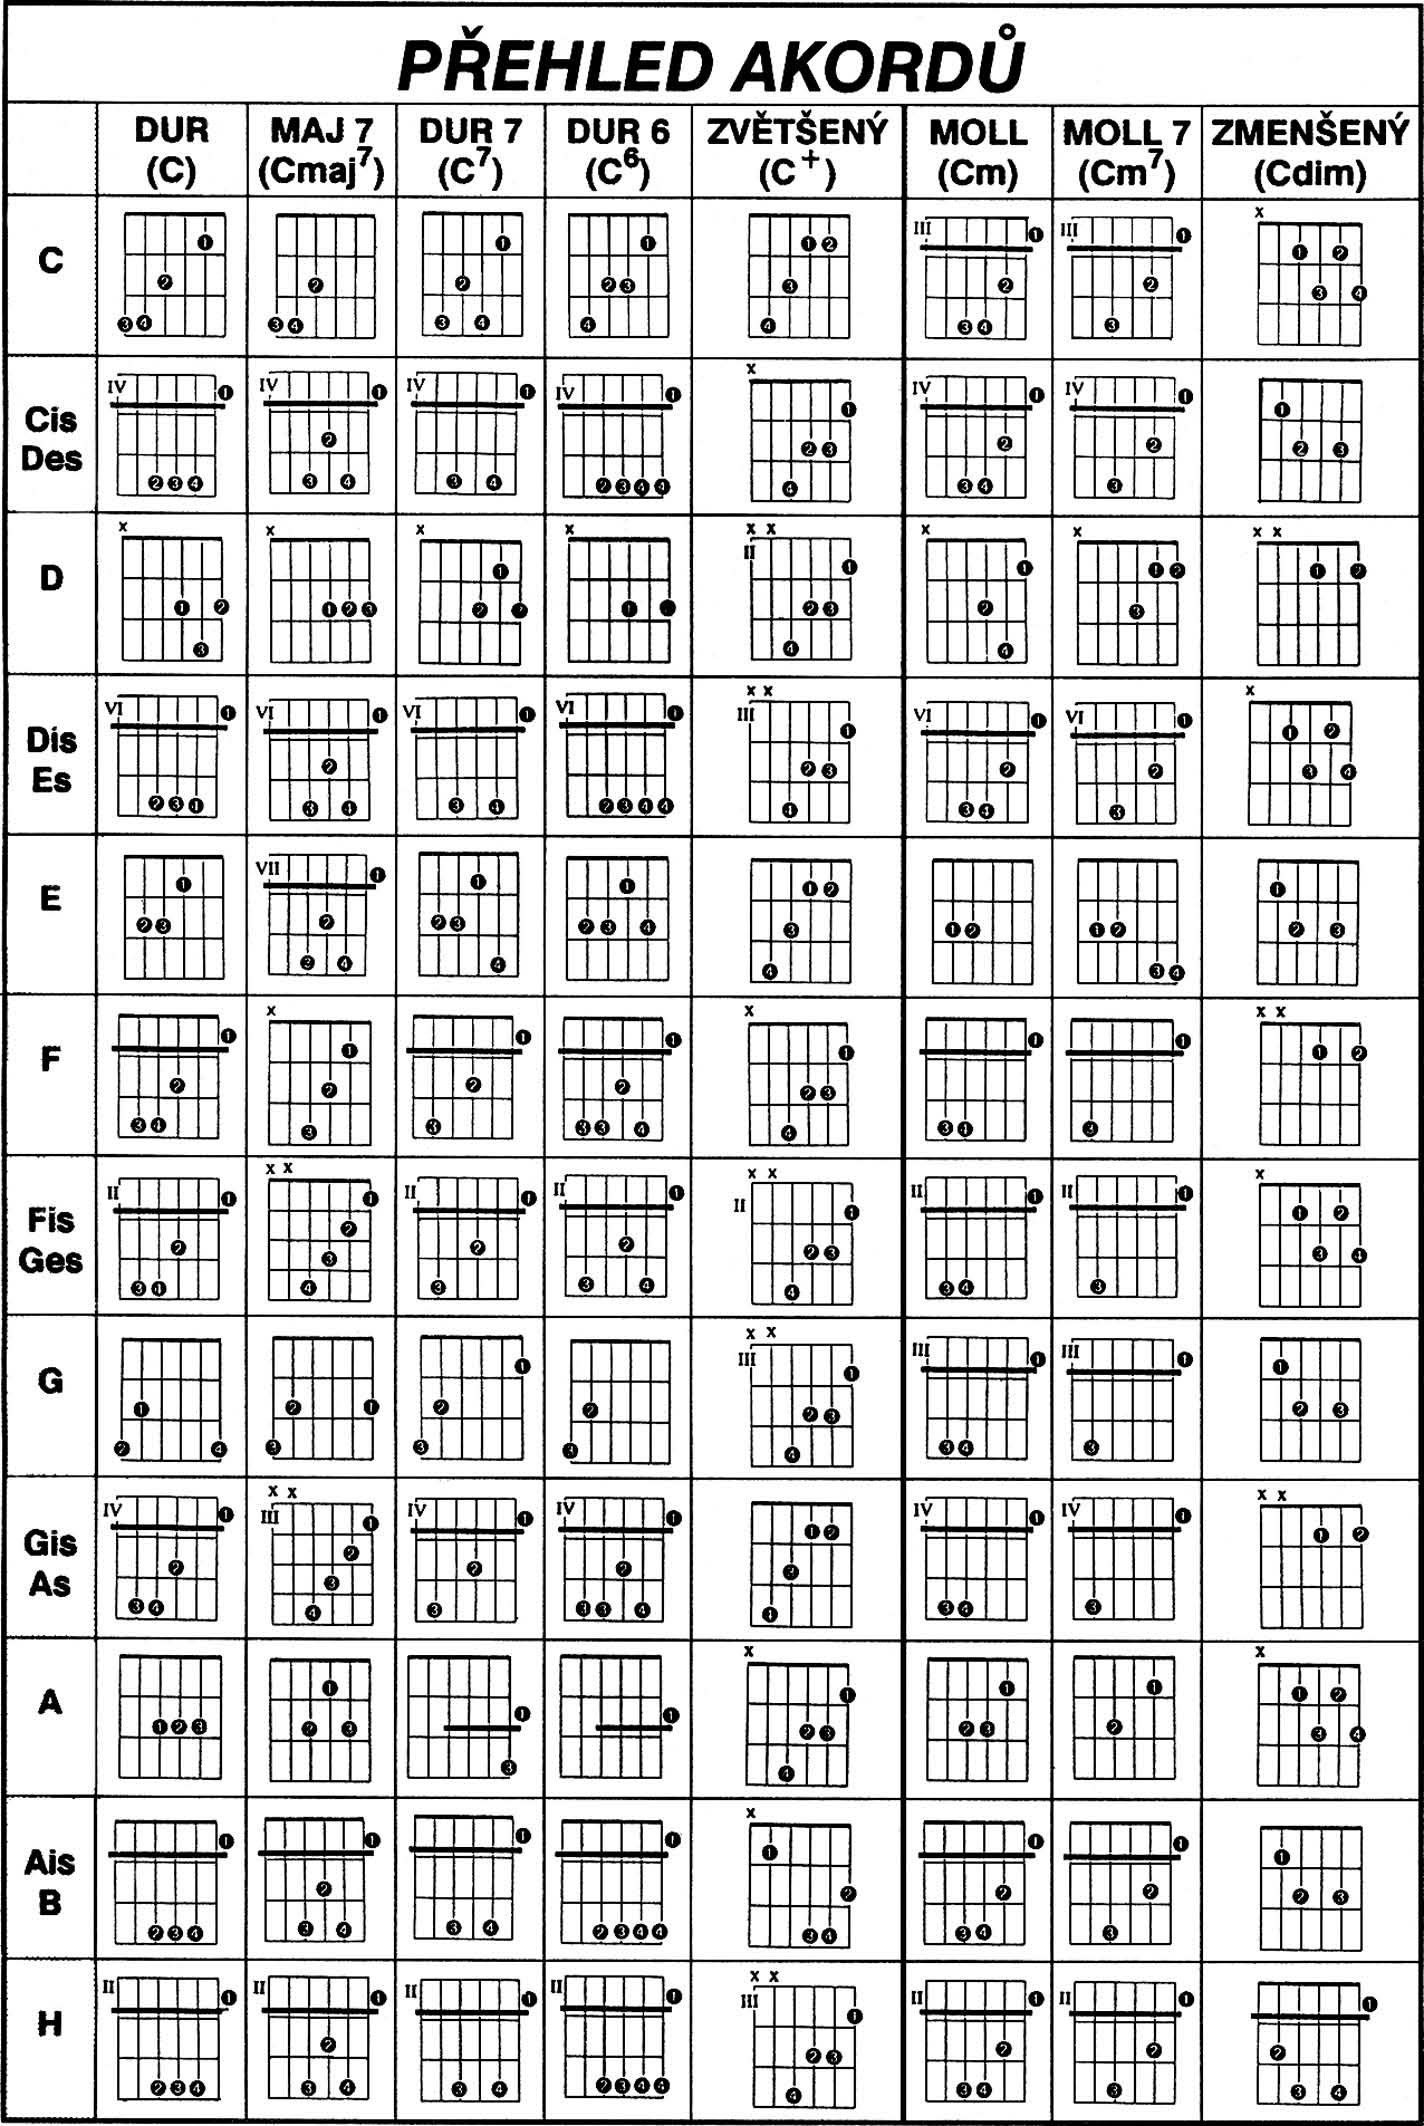
\includegraphics[width=\linewidth]{akordy.jpg}
	\end{center}
\end{figure}

\end{document}


